\documentclass[letterpaper]{article}
\usepackage[margin=1in]{geometry}
\usepackage[utf8]{inputenc}
\usepackage{textcomp}
\usepackage{amssymb}
\usepackage{natbib}
\usepackage{graphicx}
\usepackage{gensymb}
\usepackage{amsthm, amsmath, mathtools}
\usepackage[dvipsnames]{xcolor}
\usepackage{enumerate}
\usepackage{mdframed}
\usepackage[most]{tcolorbox}
\usepackage{csquotes}
% https://tex.stackexchange.com/questions/13506/how-to-continue-the-framed-text-box-on-multiple-pages

\tcbuselibrary{theorems}

\newcommand{\R}{\mathbb{R}}
\newcommand{\Z}{\mathbb{Z}}
\newcommand{\N}{\mathbb{N}}
\newcommand{\Q}{\mathbb{Q}}
\newcommand{\C}{\mathbb{C}}
\newcommand{\code}[1]{\texttt{#1}}
\newcommand{\mdiamond}{$\diamondsuit$}
\newcommand{\PowerSet}{\mathcal{P}}
\newcommand{\Mod}[1]{\ (\mathrm{mod}\ #1)}
\DeclareMathOperator{\lcm}{lcm}

%\newtheorem*{theorem}{Theorem}
%\newtheorem*{definition}{Definition}
%\newtheorem*{corollary}{Corollary}
%\newtheorem*{lemma}{Lemma}
\newtheorem*{proposition}{Proposition}


\newtcbtheorem[number within=section]{theorem}{Theorem}
{colback=green!5,colframe=green!35!black,fonttitle=\bfseries}{th}

\newtcbtheorem[number within=section]{definition}{Definition}
{colback=blue!5,colframe=blue!35!black,fonttitle=\bfseries}{def}

\newtcbtheorem[number within=section]{corollary}{Corollary}
{colback=yellow!5,colframe=yellow!35!black,fonttitle=\bfseries}{cor}

\newtcbtheorem[number within=section]{lemma}{Lemma}
{colback=red!5,colframe=red!35!black,fonttitle=\bfseries}{lem}

\newtcbtheorem[number within=section]{example}{Example}
{colback=white!5,colframe=white!35!black,fonttitle=\bfseries}{def}

\newtcbtheorem[number within=section]{note}{Important Note}{
        enhanced,
        sharp corners,
        attach boxed title to top left={
            xshift=-1mm,
            yshift=-5mm,
            yshifttext=-1mm
        },
        top=1.5em,
        colback=white,
        colframe=black,
        fonttitle=\bfseries,
        boxed title style={
            sharp corners,
            size=small,
            colback=red!75!black,
            colframe=red!75!black,
        } 
    }{impnote}
\usepackage[utf8]{inputenc}
\usepackage[english]{babel}
\usepackage{fancyhdr}
\usepackage[hidelinks]{hyperref}
\usepackage{polynom}

\pagestyle{fancy}
\fancyhf{}
\rhead{Math 187A}
\chead{March 12th, 2023}
\lhead{Course Notes}
\rfoot{\thepage}

\setlength{\parindent}{0pt}

\DeclareMathOperator{\ord}{ord}

\begin{document}

\begin{titlepage}
    \begin{center}
        \vspace*{1cm}
            
        \Huge
        \textbf{Math 187A Notes}
            
        \vspace{0.5cm}
        \LARGE
        Introduction to Cryptography
            
        \vspace{1.5cm}
            
        \vfill
            
        Winter 2023\\
        Taught by Professor Shishir (Sunny) Agrawal
    \end{center}
\end{titlepage}

\pagenumbering{gobble}

\newpage 

\pagenumbering{gobble}
\begingroup
    \renewcommand\contentsname{Table of Contents}
    \tableofcontents
\endgroup

\newpage
\pagenumbering{arabic}

\section{Introduction to Cryptography}
We begin with some common definitions.

\subsection{Terminology}
\begin{definition}{Cipher}{}
    A \textbf{cipher}, or cryptosystem, is a cryptographic method for confidential communication. 
\end{definition}
Generally, a cryptographic method includes algorithms for \emph{encryption} and \emph{decryption}, which are inverse processes that convert between plainly readable information called \emph{plaintext}\footnote{In cryptography, we use \emph{plaintext} and \emph{ciphertext} instead of \emph{plain text} and \emph{cipher text}.} and unintelligible information called \emph{ciphertext}.

\begin{definition}{Sender}{}
    A \textbf{sender}, often named ``Alice'' in abstract cryptographic discussions, \emph{encrypts} her plaintext into ciphertext. 
\end{definition}

\begin{definition}{Receiver}{}
    A \textbf{receiver}, often named ``Bob,'' \emph{decrypts} (or deciphers) the ciphertext back into plaintext. 
\end{definition}
Often times, Bob will use a \emph{key} to decrypt the message. This is sometimes known as a private key or decryption key.

\begin{definition}{Encoding}{}
    The (usually) preliminary step where a message is converted into a format which can then be encrypted is called \textbf{encoding}. 
\end{definition}
Note that encoded text is not secure; it is only secure after encryption. So, we can think of encoding as the pre-processing step. In other words, before we encrypt something, we might \emph{encode} the text so it's easier to encrypt. It should also be noted that if a message had to be encoded before encryption, then it will also need to be decoded after decryption. 

\begin{center}
    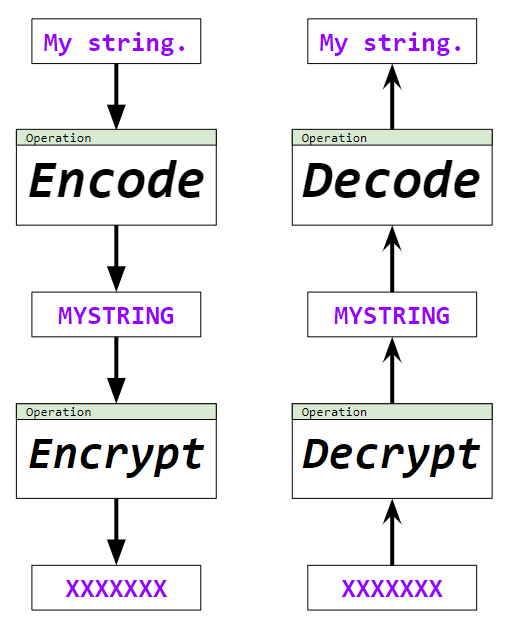
\includegraphics[scale=0.8]{assets/encode_encrypt.png}
\end{center}

\begin{definition}{Adversary}{}
    An \textbf{adversary}, often named ``Eve,'' is one whose aim is to prevent the users of a cryptosystem from achieving their goal. 
\end{definition}
In our case here, an adversary can intercept a ciphertext. Thus, the adversary will not have Bob's decryption key at the beginning. The idea is that, even if the adversary knows what cryptosystem was used to encrypt the message, if the adversary doesn't have this decryption key, she should ideally not be able to decrypt the message. If she does manage to figure out the plaintext, she has \emph{broken} the code.

\begin{definition}{Attack Model}{}
    An \textbf{attack model} specifies what Eve is allowed to do in order to break the code. 
\end{definition}
Some common attack models includes:
\begin{itemize}
    \item Ciphertext-only attack: Eve must recover the plaintext using only the ciphertext.
    \item Known-plaintext attack: Eve may have access to some information about the plaintext (e.g., knowledge of portions of the plaintext), which can be used to recover the plaintext entirely. 
    \item Chosen-plaintext attack: Eve can request or generate ciphertexts corresponding to any plaintext message of her choosing, and she can use this information to recover the plaintext.
\end{itemize}
Classical cryptography was mostly concerned with assuring security against the first two. Modern cryptography tries to assure security against the last. 


\newpage 
\section{Classical Cryptosystems}
We begin with a definition: 
\begin{definition}{$n$-gram}{}
    An $n$-gram is a sequence of $n$ letters.
\end{definition}
For example, a 1-gram is just a single letter; a 2-gram (i.e., \emph{bigram}) is a pair of letters; and so on. Generally, we can group many classical cryptosystems into a few different encryption strategies.

\begin{center}
    \begin{tabular}{|p{1in}|p{5in}|}
        \hline
        \textbf{Strategy} & \textbf{Description} \\ 
        \hline 
        Transposition & Involves rearranging units of plaintext according to some pattern. We'll see just one example of this type of cipher: rectangular transposition. \\ 
        \hline 
        Substitution & Involves replacing units of plaintext with units of ciphertext. We can further group substitution ciphers into some subtypes: 
        \begin{center}
            \begin{tabular}{|p{1in}|p{3.5in}|}
                \hline
                \textbf{Subtype} & \textbf{Description} \\ 
                \hline
                Simple \\ Substitution & In these ciphers, single letters of plaintext are replaced by ciphertext. The substitution scheme stays the same over the course of the entire message. Some examples we'll see include:
                \begin{itemize}
                    \item Masonic cipher 
                    \item Caesar cipher 
                    \item Affine cipher 
                    \item Polybius square 
                \end{itemize}
                In essence, though, there is a 1-1 relationship between the letters of the plaintext and the ciphertext alphabets. \\
                \hline 
                Polygraphic \\ Substitution & In these ciphers, groups of letters in the plaintext are replaced by ciphertext (a group of $n$ letters is called an $n$-gram).The substitution scheme stays the same over the entire message. Some examples we'll see include: 
                \begin{itemize}
                    \item Hill cipher
                    \item Playfair cipher
                \end{itemize}
                So, in essence, polygraphic substitution is just simple substitution but with \emph{groups of letters} instead of individual letters. \\ 
                \hline 
                Polyalphabetic \\ Substitution & In these ciphers, single letters in the plaintext are replaced by ciphertext, and the substitution scheme changes over the course of the message. Some examples include: 
                \begin{itemize}
                    \item Vignere cipher 
                    \item One-time pad 
                \end{itemize} 
                \\ 
                \hline 
            \end{tabular}
        \end{center}
        In practice, however, most cryptosystems employ a combination of these strategies. \\
        \hline 
    \end{tabular}
\end{center}


















\subsection{Rectangular Transposition}
\textbf{Rectangular transposition}, known also as \emph{regular columnar transposition}, is a transposition cipher. The ciphertext is obtained by \emph{permuting} the letters of the plaintext in a particular pattern. The pattern is determined by a secret \emph{keyword}. 

\bigskip 

Roughly speaking, the steps to perform rectangular transposition are as follows:
\begin{enumerate}
    \item Using the keyword, rank the letters based on alphabetical ranking. 
    \item Break up the message into groups of $n$, where $n$ is the length of the keyword.
    \item For each group, do the following: 
    \begin{itemize}
        \item Encrypting: If the $i$th letter of the keyword has rank $j$, move the $i$th letter in the group into the $j$th position.
        \item Decrypting: If the $i$th letter of the keyword has rank $j$, move the $j$th letter of each group into the $i$th position. 
    \end{itemize}
\end{enumerate}
Note that keywords with repeat letters do not work by themselves. We either need to agree not to use words with repeat letters, or remove duplicate letters from the keyword\footnote{In this course, we won't consider words with repeat letters.}.

\begin{mdframed}[]
    (Example: Encryption.) Suppose that Alice and Bob share the keyword \code{GUARD}, and that Alice wants to send the following message to Bob: 
    \begin{mdframed}
        \begin{verbatim}
Hide! The baboons are coming for you. \end{verbatim}
    \end{mdframed}

    First, we'll \textbf{encode} the message so that it's easier to encrypt. In our example, we'll remove all spaces and punctuation. 
    \begin{mdframed}
        \begin{verbatim}
HIDETHEBABOONSARECOMINGFORYOU \end{verbatim}
    \end{mdframed}
    Now that encoding is done, we still need to encrypt the message. Notice how the keyword \code{GUARD} has 5 letters; we can break the message up into 5-grams and then stack them into rows:
    \begin{mdframed}
        \begin{verbatim}
HIDET
HEBAB
OONSA
RECOM
INGFO
RYOU\end{verbatim}
    \end{mdframed}
    We then need to insert some random letters at the end of the message so every row has an equal number of letters. Let's use \code{Q}:
    \begin{mdframed}
        \begin{verbatim}
HIDET
HEBAB
OONSA
RECOM
INGFO
RYOUQ\end{verbatim}
    \end{mdframed}
    Now, we begin the \textbf{encryption} process by rearranging the letters in each row based on the alphabetical ranking of the letters of the keyword \code{GUARD}. 
    \begin{center}
        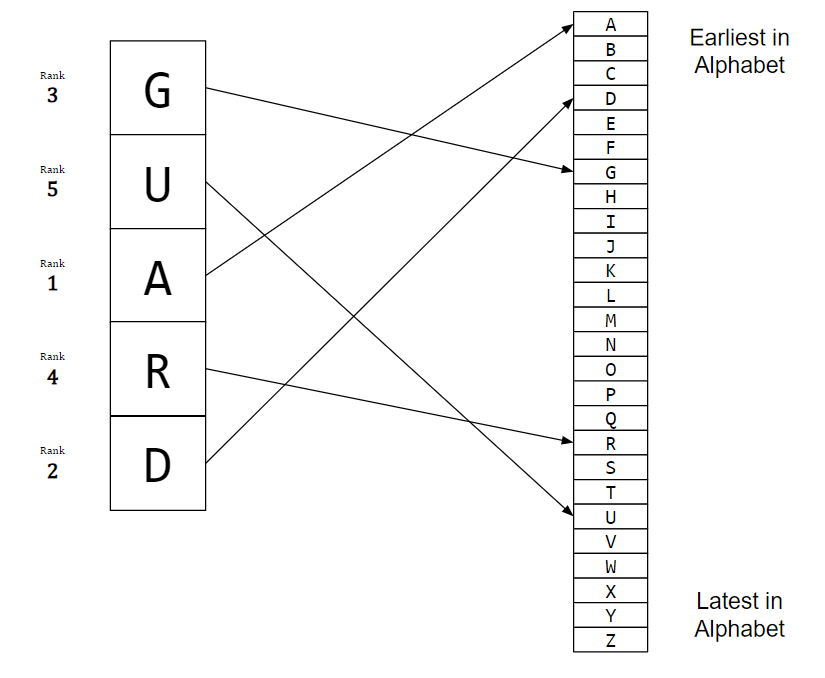
\includegraphics[scale=0.7]{assets/rank_crypto.png}
    \end{center}
    We note that the alphabetical rankings of the letters of this keyword are 3, 5, 1, 4, 2. We can see this as a \emph{permutation}; that is, 
    \[1 \mapsto 3 \qquad 2 \mapsto 5 \qquad 3 \mapsto 1 \qquad 4 \mapsto 4 \qquad 5 \mapsto 2\]
    \textbf{The idea for encryption is that, for each column $i$, we'll send that column to whatever is mapped by the permutation above.} Going back to the stack of letters we have, we can label each individual column:
    \begin{mdframed}
        \begin{verbatim}
plaintext 
position    1 2 3 4 5
            H I D E T
            H E B A B
            O O N S A
            R E C O M
            I N G F O
            R Y O U Q\end{verbatim}
    \end{mdframed}
    The idea is that 
    \begin{itemize}
        \item we can put all letters under position 1 in the plaintext stack to position \textbf{3} of the ciphertext stack, 
        \item we can put all letters under position 2 in the plaintext stack to position \textbf{5} of the ciphertext stack, 
        \item we can put all letters under position 3 in the plaintext stack to position \textbf{1} of the ciphertext stack, 
        \item we can put all letters under position 4 in the plaintext stack to position \textbf{4} of the ciphertext stack, 
        \item we can put all letters under position 5 in the plaintext stack to position \textbf{2} of the ciphertext stack.
    \end{itemize}
    The process, visually, would look like: 
    \begin{center}
        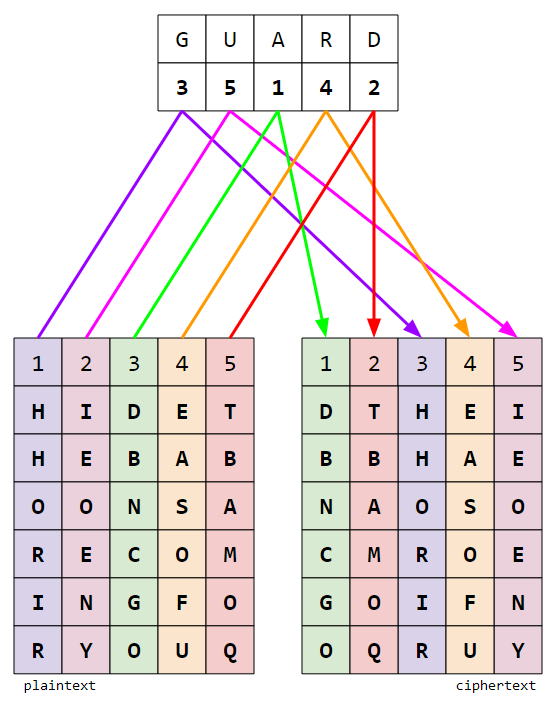
\includegraphics[scale=0.7]{assets/trans_encrypt.png}
    \end{center}
    Therefore, the ciphertext stack would look like: 
    \begin{mdframed}
        \begin{verbatim}
DTHEI
BBHAE
NAOSO
CMROE
GOIFN
OQRUY\end{verbatim}
    \end{mdframed}
    Undoing the stacking gives us the ciphertext: 
    \begin{mdframed}
        \begin{verbatim}
DTHEIBBHAENAOSOCMROEGOIFNOQRUY\end{verbatim}
    \end{mdframed}
\end{mdframed}
\textbf{Remark:} An easy way to run through the process is to create two ``groups,'' side-by-side. The first group will be the plaintext stack, and the second group will be the ciphertext text. Then, label each column of the first group with the \textbf{alphabetical ranking} of the keyword. Label each column of the second group with \textbf{12345}. Finally, map each column from the first group to the second group based on the label. 
\begin{center}
    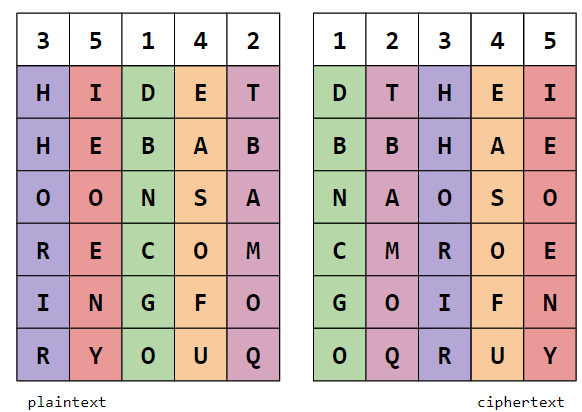
\includegraphics[scale=0.7]{assets/trans_encrypt2.png}
\end{center} 

Decrypting is merely the inverse of the encryption process.
\begin{mdframed}
    (Example: Decryption.) Consider the above example again. Suppose Alice successfully sends the following ciphertext to Bob:
    \begin{mdframed}
        \begin{verbatim}
DTHEIBBHAENAOSOCMROEGOIFNOQRUY\end{verbatim}
    \end{mdframed}
    Bob knows that the keyword is \code{GUARD}. He can use this keyword to decrypt the message. He can begin by taking the letters of the ciphertext and stacking them into rows of 5, since \code{GUARD} has 5 letters:
    \begin{mdframed}
        \begin{verbatim}
DTHEI
BBHAE
NAOSO
CMROE
GOIFN
OQRUY\end{verbatim}
    \end{mdframed}
    Bob also knows the alphabetical ranking of the letters of \code{GUARD} (which is the same rankings as described above). In particular, the alphabetical ranking is \code{35142}. So, we need to do the following: 
    \begin{itemize}
        \item The letters in position 1 of the ciphertext stack needs to be moved to position \textbf{3},
        \item the letters in position 2 of the ciphertext stack needs to be moved to position \textbf{5},
        \item the letters in position 3 of the ciphertext stack needs to be moved to position \textbf{1},
        \item the letters in position 4 of the ciphertext stack needs to be moved to position \textbf{4},
        \item the letters in position 5 of the ciphertext stack needs to be moved to position \textbf{2}. 
    \end{itemize}
    
    The process, visually, would look like: 
    \begin{center}
        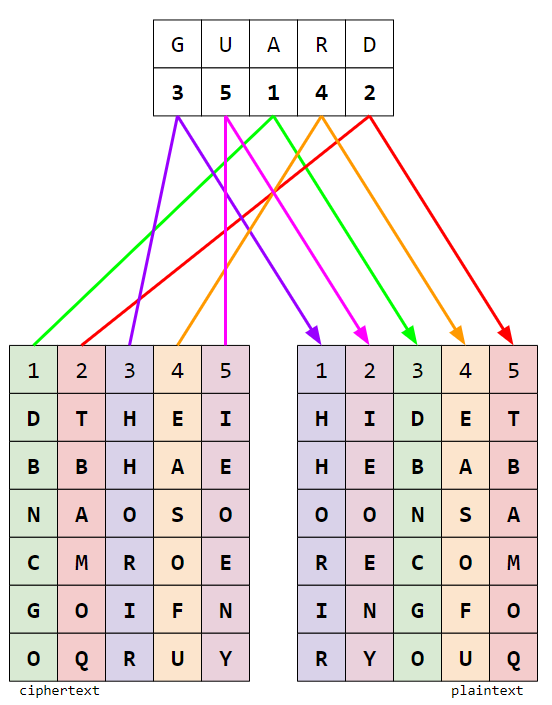
\includegraphics[scale=0.7]{assets/trans_decrypt.png}
    \end{center}
    Undoing the stacking gives us:
    \begin{mdframed}
        \begin{verbatim}
HIDETHEBABOONSARECOMINGFORYOUQ\end{verbatim}
    \end{mdframed}
    At this point, Bob needs to make an educated guess as to what the encoded message says (recall that we had to encode the message before encrypting it). By removing the \code{Q} and correctly punctuating the message, we get 
    \begin{mdframed}
        \begin{verbatim}
Hide! The baboons are coming for you.\end{verbatim}
    \end{mdframed}
\end{mdframed}
\textbf{Remark:} We can easily decrypt an encrypted word by doing the inverse of what we did above. Create two ``groups,'' side-by-side. The first group will be the ciphertext stack, and the second group will be the plaintext text. Then, label each column of the first group with \textbf{12345}. Label each column of the second group with the \textbf{alphabetical ranking} of the keyword. Finally, map each column from the first group to the second group based on the label. 
\begin{center}
    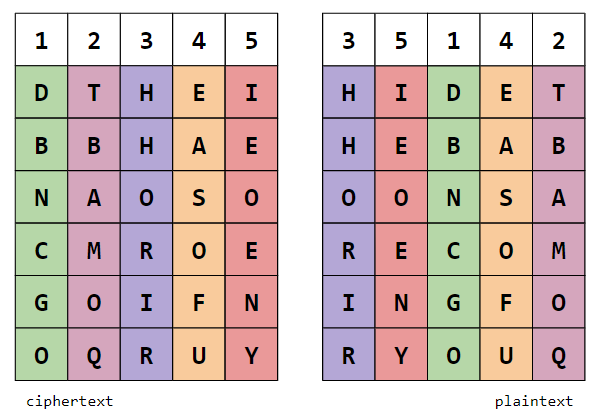
\includegraphics[scale=0.7]{assets/trans_decrypt2.png}
\end{center} 

\begin{mdframed}[]
    (Exercise: Encryption.) \emph{Encrypt the message \code{There is always hope.} using the keyword \code{CRASH}.}

    \begin{mdframed}
        First, we encode the message so that we can easily encrypt it: 
        \begin{mdframed}
            \begin{verbatim}
THEREISALWAYSHOPE\end{verbatim}
        \end{mdframed}

        Noting that \code{CRASH} has length 5, we break the now encoded message into groups of 5 letters (5-grams):
        \begin{mdframed}
            \begin{verbatim}
THERE
ISALW
AYSHO
PE\end{verbatim}
        \end{mdframed}
        
        Let's now add nonsense letters at the end of the last row so every row has 5 letters: 
        \begin{mdframed}
            \begin{verbatim}
THERE
ISALW
AYSHO
PEABC\end{verbatim}
        \end{mdframed}

        Now, we note the alphabetical ranking of each letter in \code{CRASH}:
        \[C \mapsto 2 \quad R \mapsto 4 \quad A \mapsto 1 \quad S \mapsto 5 \quad H \mapsto 3.\]
        Using the streamlined way discussed above, we have 
        \begin{mdframed}
            \begin{verbatim}
2 4 1 5 3 | 1 2 3 4 5
T H E R E | E T E H R
I S A L W | A I W S L
A Y S H O | S A O Y H
P E A B C | A P C E B\end{verbatim}
        \end{mdframed}
        Unstacking the new rows gives us the ciphertext:
        \begin{mdframed}
            \begin{verbatim}
ETEHRAIWSLSAOYHAPCEB\end{verbatim}
        \end{mdframed}
    \end{mdframed}
\end{mdframed}


\begin{mdframed}[nobreak=true]
    (Exercise: Decryption.) \emph{Decrypt the message \code{ETIHGFREAFRSLAESOXOE} using the keyword \code{CRASH}.}

    \begin{mdframed}
        Begin by grouping the letters into 5-grams, since \code{CRASH} has length 5:
        \begin{mdframed}
            \begin{verbatim}
ETIHG
FREAF
RSLAE
SOXOE\end{verbatim}
        \end{mdframed}
        Recall that the alphabetical ranking of each letter in \code{CRASH} is \code{24153}. Using the streamlined way discussed above, we have 
        \begin{mdframed}
            \begin{verbatim}
1 2 3 4 5    2 4 1 5 3
E T I H G -> T H E G I 
F R E A F -> R A F F E 
R S L A E -> S A R E L 
S O X O E -> O O S E X \end{verbatim}
        \end{mdframed}
        Unstacking the new rows gives us the plaintext:
        \begin{mdframed}
            \begin{verbatim}
THEGIRAFFESARELOOSEX\end{verbatim}
        \end{mdframed}
        Decoding the message gives us: 
        \begin{mdframed}
            \begin{verbatim}
The giraffes are loose.\end{verbatim}
        \end{mdframed}
    \end{mdframed}

\end{mdframed}

\begin{mdframed}
    (Exercise.) Encrypt the message \code{Meet at the trolley station.} using keyword \code{UCSD}.

    \begin{mdframed}
        Encoding, grouping the resulting letters into groups of 4, and adding a nonsense letter gives us: 
        \begin{verbatim}
MEET
ATTH
ETRO
LLEY
STAT
IONX\end{verbatim}
        Noting that the alphabetical ranking of \code{UCSD} is \code{4132}, we can use the streamlined way discussed above to get the encrypted result:
        \begin{mdframed}
            \begin{verbatim}
4 1 3 2    1 2 3 4
M E E T -> E T E M
A T T H -> T H T A
E T R O -> T O R E
L L E Y -> L Y E L
S T A T -> T T A S
I O N X -> O X N I\end{verbatim}
        \end{mdframed}
        Unstacking the result gives us:
        \begin{mdframed}
            \begin{verbatim}
/ETEMTHTATORELYELTTASOXNI\end{verbatim}
        \end{mdframed}
    \end{mdframed}
\end{mdframed}

\begin{mdframed}
    (Exercise.) Alice and Bob share the keyword \code{ZEUS}. Alice uses rectangular transposition to encrypt the following nonsense message: 
    \begin{verbatim}
MTSQAGXY\end{verbatim}
    What is the corresponding ciphertext? 
    \begin{mdframed}
        Encoding, grouping the resulting letters into groups of 4, and adding a nonsense letter gives us: 
        \begin{mdframed}
            \begin{verbatim}
MTSQ
AGXY\end{verbatim}
        \end{mdframed}
        Noting that the alphabetical ranking of \code{ZEUS} is \code{4132}, we can use the streamlined way discussed above to get the encrypted result:
        \begin{mdframed}
            \begin{verbatim}
4 1 3 2    1 2 3 4
M T S Q -> T Q S M
A G X Y -> G Y X A\end{verbatim}
        \end{mdframed}
        Unstacking the result gives us:
        \begin{mdframed}
            \begin{verbatim}
TQSMGYXA\end{verbatim}
    \end{mdframed}
    \end{mdframed}
\end{mdframed}

\begin{mdframed}
    (Exercise.) The following message was encrypted using rectangular transposition with the keyword \code{SNAKE}. What is the plaintext? 
    \begin{verbatim}
        DSUEMSEDIAJQQDA\end{verbatim}
    
    \begin{mdframed}
        \code{SNAKE} has alphabetical ranking \code{54132}. With this in mind, stacking the letters of the encrypted message into groups of 5 and then running the streamlined process gives us: 
        \begin{mdframed}
\begin{verbatim}
1 2 3 4 5    5 4 1 3 2   
D S U E M -> M E D U S
S E D I A -> A I S D E
J Q Q D A -> A D J Q Q\end{verbatim}
        \end{mdframed}

        Unstacking the result gives us: 
        \begin{mdframed}
\begin{verbatim}
MEDUSAISDEADJQQ\end{verbatim}
        \end{mdframed}
        Decoding gives us: 
        \begin{mdframed}
\begin{verbatim}
Medusa is dead.\end{verbatim}
        \end{mdframed}
    \end{mdframed}
\end{mdframed}


\subsection{Masonic Cipher}
The masonic cipher (also known as the \emph{pigpen cipher} or \emph{tic-tac-toe cipher}) is a simple substitution cipher that replaces individual letters with certain geometric shapes.

\bigskip 

For example, consider the following diagram, which represents a Masonic cipher for the English letters:
\begin{center}
    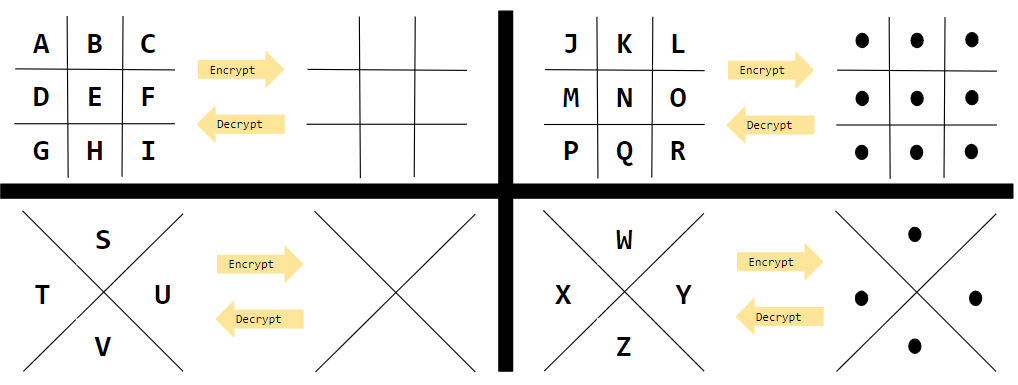
\includegraphics[scale=0.75]{assets/masonic_ex1.png}
\end{center}
The idea is that we can replace a letter (e.g., \code{A}) with a corresponding geometric shape (e.g., the backwards \code{L} represented by the top-left part of the grid.) 

\bigskip 

Some other examples based on the above cipher are shown below:
\begin{center}
    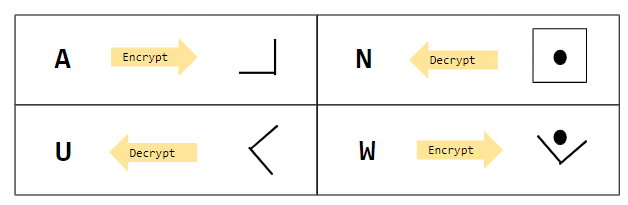
\includegraphics[scale=0.9]{assets/masonic_ex2.png}
\end{center}
Note that there is \emph{no key} associated with this cipher. There is only a decryption function (which is just mapping the geometric shape back to the letter). Therefore, the adversary, who knows that a message was encrypted using a masonic cipher, can recover the plaintext easily. 


\subsection{Caesar Cipher}
The Caesar cipher, also known as a \emph{shift cipher}, is a simple substitution cipher that \emph{shifts} a letter by some amount $n$. Hence, the key for this cipher is an integer $n$. The idea is that we initially assign each letter an integer, perhaps by their alphabetical ranking (e.g., $A$ is 0, $B$ is 1, and so on.) If we want to shift the letters by some number, we can just ``move'' the letters by that amount. If a letter gets a new integer that's greater than 25, we can ``wrap'' the letter back.  

\bigskip 

Consider the following diagram, which shows the correspondence between the plaintext alphabet and the ciphertext alphabet.
\begin{center}
    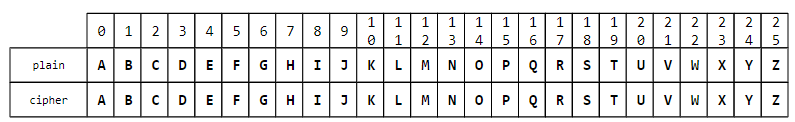
\includegraphics[scale=0.75]{assets/ceasar_1.png}
\end{center}
In this particular diagram, when we apply a shift, we apply the shift to the \emph{plain} row. By doing this, we can translate whatever plaintext we have to ciphertext. 

\begin{mdframed}
    (Example.) If we shift each letter by 3 (i.e., $n = 3$), we have 
    \begin{center}
        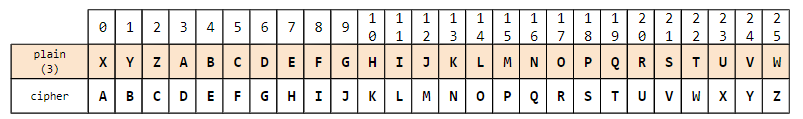
\includegraphics[scale=0.7]{assets/ceasar_2.png}
    \end{center}
    Notice how $A$ now corresponds to 3. Recall that $A$'s original position was 0; if we shift each letter by 3, we essentially add 3 to $A$'s original position to get the new position 
    \[0 + 3 = 3.\]
    The same idea applies to any other letter. One key thing to notice is how $X$, $Y$, and $Z$ were \emph{wrapped back} to the beginning. In any case, let's see how translation would work in this case: 
    \begin{itemize}
        \item To convert a letter from plaintext to ciphertext, look for the letter in the(shifted) plaintext row and then look at the corresponding ciphertext column. For example, $R$ in plaintext would become $U$ in ciphertext. 
        \item To convert a letter from ciphertext to plaintext, look for the letter in the ciphertext row and then look at the corresponding (shifted) plaintext column. For example, $U$ in ciphertext becomes $R$ in plaintext. 
    \end{itemize}
\end{mdframed}

\begin{mdframed}
    (Example.) If we shift each letter by -2 (i.e., $n = -2$), we have 
    \begin{center}
        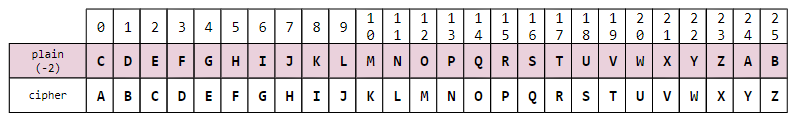
\includegraphics[scale=0.7]{assets/ceasar_3.png}
    \end{center}
\end{mdframed}

As with rectangular transposition, we should encode the message by removing any non-alphabetic characters and capitalizing everything. 

\begin{mdframed}
    (Exercise.) 
    \begin{itemize}
        \item \emph{Using a shift of 3, encrypt the message \code{Meet at La Jolla Shores.}}
        \begin{mdframed}
            Encoding the message gives us \code{MEETATLAJOLLASHORES}. Then, we can use the example above (with the shift of 3) to give us the proper correspondence.
            \begin{verbatim}
    plain       M E E T A T L A J O L L A S H O R E S
    cipher      P H H W D W O D M R O O D V K R U H V\end{verbatim}
            This gives us \code{PHHWDWODMROODVKRUHV}.
        \end{mdframed}
        \item \emph{Using a shift of 3, decrypt the message \code{PHHWDWVXQJRGODZQ}}
        \begin{mdframed}
            Using the example above (with the shift of 3), we have
            \begin{verbatim}
    cipher      P H H W D W V X Q J R G O D Z Q
    plain       M E E T A T S U N G O D L A W N\end{verbatim}
            Decoding this gives us \code{Meet at Sun God Lawn.}
        \end{mdframed}
    \end{itemize}
\end{mdframed}

\begin{mdframed}
    (Exercise.) \emph{You are Eve. You have just intercepted the following message that Alice was trying to send to Bob: \code{Q TQDM IB QPWCAM}. You know that Alice used a Caesar cipher, but she didn't remove spaces before encrypting: she left the spaces in her original message as-is. What is the original message?}
    
    \begin{mdframed}
        \code{Q} itself could be a word; specifically, it could either be \code{A} or \code{I}. We can try to figure out what the message by guessing which word the first word could be. 
        \begin{itemize}
            \item If \code{Q} maps to \code{A}, then we have 
            \begin{center}
                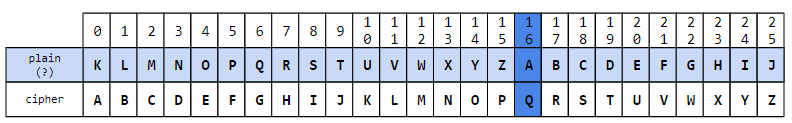
\includegraphics[scale=0.6]{assets/ceasar_4.png}
            \end{center}
            Partially decrypting the ciphertext gives us \code{A DANW}, but \code{DANW} is meaningless. Therefore, it cannot be \code{A}. 

            \item If \code{Q} maps to \code{I}, then we have
            \begin{center}
                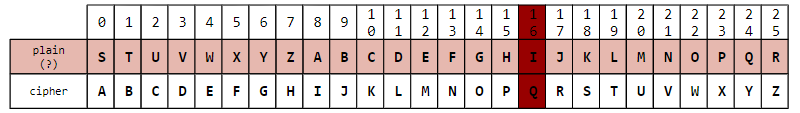
\includegraphics[scale=0.6]{assets/ceasar_5.png}
            \end{center}
            Decrypting this gives us: 
            \begin{verbatim}
                I LIVE AT IHOUSE\end{verbatim}
        \end{itemize}
        Therefore, the message is \code{I LIVE AT IHOUSE}. The shift was 8.
    \end{mdframed}
\end{mdframed}


\begin{mdframed}
    (Exercise.) Alice encrypts the following message using a Caesar cipher with a shift of 1. 
    \begin{verbatim}
Zeus is hiding in a cave \end{verbatim}
    What is the corresponding ciphertext? 
    \begin{mdframed}
        \begin{verbatim}
plain       ZEUSISHIDINGINACAVE
cipher      AFVTJTIJEJOHJOBDBWF\end{verbatim}
        Essentially, we just move all letters forward by 1.
    \end{mdframed}
\end{mdframed}


\subsection{Interlude: Modular Arithmetic}
One fundamental idea in number theory, which is used in cryptography, is modular arithmetic. 

\subsubsection{Quotients and Remainders}

\begin{lemma}{Euclid's Division}{}
    For any integer $a$ and positive integer $n$, there exists a unique pair of integers $q$ and $r$ such that $0 \leq r < n$ and $a = qn + r$. The integers $q$ and $r$ are called the quotient and remainder, respectively. We also write $a \Mod{n}$ to refer to the remainder.
\end{lemma}
For the proof, the deal is that we can keep subtracting, or adding, $n$ from $a$ until we end up in the range $[0, n)$. Therefore, the number of times we had to subtract, or add, $n$ is the \emph{quotient}, and the number in the range $[0, n)$ that we end up with at the end is the \emph{remainder}. 

\begin{mdframed}
    (Example.) Divide $a = 17$ by $n = 5$. Find the quotient and remainder.
    
    \bigskip 

    Using the proof idea, we note that: 
    \begin{itemize}
        \item Subtracting 5 to $a$ once gives us 12. 
        \item Subtracting 5 to $a$ twice gives us 7.
        \item Subtracting 5 to $a$ thrice gives us 2.
    \end{itemize}
    It took us 3 subtractions to get to a number that's in the range $[0, 5)$, so the quotient is $\boxed{3}$ and the remainder is $\boxed{2}$. 
\end{mdframed}
We should note that this is pretty standard when $a \geq 0$. However, for $a < 0$, it might be less familiar, albeit the same process.

\begin{mdframed}
    (Example.) Divide $a = -7$ by $n = 5$. Find the quotient and remainder.

    \bigskip 

    Using the proof idea, we note that: 
    \begin{itemize}
        \item Adding 5 to $a$ once gives us 2.
        \item Adding 5 to $a$ twice gives us 3. 
    \end{itemize}
    It took us 2 additions to get to a number that's in the range $[0, 5)$, so the quotient is $\boxed{-2}$ (because we had to \emph{add}, not subtract) and the remainder is $\boxed{3}$. 
\end{mdframed}

\textbf{Remark:} 
\begin{itemize}
    \item If we have to \textbf{add} $n$ to $a$ $x$ times to get a number that's in the range $[0, n)$, then our final quotient will be negative (that is, $-x$).
    \item If we have to \textbf{subtract} $n$ from $a$ $x$ times to get a number that's in the range $[0, n)$, then our final quotient will be positive (that is, $x$).
\end{itemize}

\begin{mdframed}
    (Exercise.) For each of the following, calculate the quotient and remainder when $a$ is divided by $n$. Do these calculations by hand. 
    \begin{itemize}
        \item $a = 13$, $n = 3$.
        \begin{mdframed}
            We know that $13 / 3 = 4$, and $13 - (3 \cdot 4) = 1 \in [0, 3)$. So, the quotient is \boxed{4} and the remainder is \boxed{1}. 
        \end{mdframed}
        \item $a = 134$, $n = 10$.
        \begin{mdframed}
            We know that $134 / 10 = 13$ and $134 - (10 \cdot 13) = 4 \in [0, 10)$. So, the quotient is \boxed{13} and remainder is \boxed{4}.
        \end{mdframed}
        \item $a = -37$, $n = 10$.
        \begin{mdframed}
            We know that we need to add $n$ to $a$ \textbf{4} times to get a number, $3$, that is in the range $[0, 10)$. To be precise, 
            \[-37 + 10 + 10 + 10 + 10 = -37 + 40 = 3 \in [0, 10).\]
            Therefore, the quotient is \boxed{-4} and the remainder is \boxed{3}. 
        \end{mdframed}
        \item $a = -15$, $n = 60$.
        \begin{mdframed}
            We have to add $n$ to $a$ \textbf{1} time to get $45 \in [0, 60)$. Therefore, the quotient is \boxed{-1} and the remainder is \boxed{45}.
        \end{mdframed}
        \item $a = 13$, $n = 12$.
        \begin{mdframed}
            We know that $13 / 12 = 1$ and $13 - (12 \cdot 1) = 1$. So, the quotient is \boxed{1} and the remainder is \boxed{1}.
        \end{mdframed}
    \end{itemize}
\end{mdframed}

\begin{mdframed}
    (Exercise.) What is $-13 \Mod{5}$?
    \begin{mdframed}
        \[-13 + 5 + 5 + 5 = 2 \in [0, 5),\]
        so the quotient is $-3$ (since we had to perform 3 additions) and the remainder is \boxed{2}. Therefore, 
        \[-13 \Mod{5} = 2.\]
    \end{mdframed}
\end{mdframed}

\begin{proposition}
    Suppose $a$ and $n$ are integers and $n > 0$. All the following statements are equivalent:
    \begin{itemize}
        \item $a \Mod{n} = 0$.
        \item There is no remainder when $a$ is divided by $n$. 
        \item $a$ is a multiple of $n$. 
        \item $a$ is divisible by $n$. 
        \item $n$ is a divisor of $a$. 
        \item $n$ is a factor of $a$. 
        \item $n$ divides $a$ (in notation\footnote{Note that $\vert$ is read as ``\emph{divides}.''}: $n \vert a$).
        \item $a / n$ is an integer.
    \end{itemize}
\end{proposition}

\subsubsection{Congruences}
\begin{definition}{Congruence}{}
    Fix a positive integer $n$. If $a$ and $b$ are integers, we say that ``$a$ is \textbf{congruent} to $b$ mod $n$,'' or that ``$a$ and $b$ are congruent mod $n$,'' if $a$ and $b$ have the same remainder when each is divided by $n$. This can be denoted in symbols as follows: 
    \[a \equiv b \Mod{n}.\] 
\end{definition}
For example, $19 \equiv 7 \Mod{4}$ since $19$ and $7$ both have remainder 3 when divided by 4. Observe also that $19 - 7 = 12$ is a multiple of 4. This can be generalized: 

\begin{lemma}{}{}
    Fix a positive integer $n$. Two integers $a$ and $b$ are congruent mod $n$ if and only if $a - b$ is a multiple of $n$.
\end{lemma}

\begin{proof}
    Divide $a$ and $b$ by $n$ to write $a = q_1 n + r_1$ and $b = q_2 n + r_2$. If \[a \equiv b \Mod{n},\] this by definition means that $r_1 = r_2$ so 
    \[a - b = (q_1 n + r_1) - (q_2 n + r_2) = q_1 n - q_2 n = n(q_1 - q_2).\]
    So, $a - b$ is a multiple of $n$. Conversely, suppose $a - b$ is a multiple of $n$. Then, 
    \[(a - b) - (q_1 - q_2)n = ((q_1 n + r_1) - (q_2 n + r_2)) - (q_1 - q_2)n = r_1 - r_2\]
    is a multiple of $n$. Since $0 \leq r_1, r_2 < n$, however, we must have $|r_1 - r_2| < n$. The only way that $r_1 - r_2$ can be a multiple of $n$ is if $r_1 - r_2 = 0$, i.e., if $r_1 = r_2$. That means $a \equiv b \Mod{n}$. 
\end{proof}

\begin{theorem}{Modular Arithmetic Theorem}{}
    Fix a positive integer $n$. Suppose $a$, $a'$, $b$, $b'$ are integers such that 
    \[a \equiv a' \Mod{n}\]
    \[b \equiv b' \Mod{n}\]
    and $k$ is any positive integer. Then, all of the following are also true: 
    \[a + b \equiv a' + b' \Mod{n}\]
    \[a - b \equiv a' - b' \Mod{n}\]
    \[ab \equiv a'b' \Mod{n}\]
    \[a^k \equiv (a')^k \Mod{n}\]
\end{theorem}

\begin{mdframed}
    (Exercise.) Use the Modular Arithmetic Theorem to quickly calculate the following. 
    \begin{itemize}
        \item $417 \cdot 22 \Mod{10}$.
        \begin{mdframed}
            \begin{equation*}
                \begin{aligned}
                    417 \cdot 22 &\equiv 7 \cdot 2  \\ 
                        &= 14 \\ 
                        &\equiv 4 \Mod{10}.
                \end{aligned}
            \end{equation*}
        \end{mdframed}
        \item $333333 + 666 \Mod{3}$.
        \begin{mdframed}
            \begin{equation*}
                \begin{aligned}
                    333333 + 666 &\equiv 0 + 0 \\ 
                        &\equiv 0 \Mod{3}.
                \end{aligned}
            \end{equation*}
        \end{mdframed}
        \item $7^{202320232023} \Mod{6}$. 
        \begin{mdframed}
            \begin{equation*}
                \begin{aligned}
                    7^{202320232023} &= 7 \cdot 7 \cdot \hdots \cdot 7 \\ 
                        &\equiv 1 \cdot 1 \cdot \hdots \cdot 1 \\ 
                        &= 1 \Mod{6}.
                \end{aligned}
            \end{equation*}
        \end{mdframed}
        \item What is $5^{2023202320232023} \Mod{6}$?
        \begin{mdframed}
            \begin{equation*}
                \begin{aligned}
                    5^{2023202320232023} &= 5 \cdot 5 \cdot \hdots \cdot 5 \\ 
                        &\equiv (-1) \cdot (-1) \cdot \hdots \cdot (-1) \\ 
                        &= (-1)^{2023202320232023} \\ 
                        &\equiv -1 \\ 
                        &\equiv 5 \Mod{6}.
                \end{aligned}
            \end{equation*}
            Therefore, the answer is \boxed{5}.
        \end{mdframed}
    \end{itemize}
\end{mdframed}

\begin{mdframed}
    (Exercise.) Fix positive integers $k$ and $n$. Suppose $a$ and $a'$ are integers such that $a \equiv a' \Mod{n}$. It is not true in general that $k^a \equiv k^{a'} \Mod{n}$. Show this by example: in other words, find $k$, $n$, $a$, and $a'$ such that $a \equiv a' \Mod{n}$ but $k^a \not\equiv k^{a'} \Mod{n}$. 

    \begin{mdframed}
        Let $k = 2$, $n = 5$, $a = 6$, and $a' = 1$ so that 
        \[6 \equiv 1 \Mod{5}.\]
        Then, we note that 
        \[k^a = 2^6 = 64\]
        and 
        \[k^{a'} = 2^1 = 2.\]
        From this, it's clear that 
        \[64 \not\equiv 2 \Mod{5}.\]
    \end{mdframed}
\end{mdframed}

\begin{mdframed}[nobreak=true]
    (Exercise.) \emph{Suppose that the number $273x49y5$, where $x$ and $y$ are unknown digits, is divisible by 495. Find $x$ and $y$.}
    \begin{mdframed}
        We are asked to solve 
        \[273x49y5 \equiv 0 \mod{495}.\]

        We can write $273x49y5$ as 
        \[20000000 + 7000000 + 300000 + 10000x + 4000 + 900 + 10000y + 5.\]
        With this in mind, we have
        \begin{equation*}
            \begin{aligned}
                20000000 &+ 7000000 + 300000 + 10000x + 4000 + 900 + 10y + 5 \\ 
                    &\equiv 20 + 205 + 30 + 100x + 40 + 405 + 10y + 5 \\ 
                    &= 705 + 100x + 10y \\ 
                    &\equiv 210 + 100x + 10y \mod{495}.
            \end{aligned}
        \end{equation*}
        We note that the next multiple of 495 is 990. So, effectively, we want to find some $x$ and $y$ such that $0 \leq x < 10$ and $0 \leq y < 10$ and
        \[210 + 100x + 10y = 990.\]
        This gives us 
        \[100x + 10y = 780.\]
        One obvious solution is $x = 7$ and $y = 8$. 
    \end{mdframed}
\end{mdframed}


\subsubsection{Revisiting the Caesar Cipher}
Suppose we identify the letters $A$ through $Z$ with the numbers 0 through 25. In other words, we have $A \mapsto 0$, $B \mapsto 1$, and so on. Suppose we want to apply the Caesar cipher with a shift of 5 to encrypt the letter $Y$. Consider the following 
\[E(x) = (x + 5) \Mod{26}.\]
We note that $Y$ corresponds to the number 24. Then, it follows that 
\[E(24) = (24 + 5) \Mod{26} = 29 \Mod{26} = 3.\]
The number 3 corresponds to the letter $D$, the desired result. In other words, if we can identify the letters with numbers, the function $E$ is the encryption function of the Caesar cipher with a shift of 5.  

\bigskip 

The decryption function is given by 
\[D(y) = (y - 5) \Mod{26}.\]
So, if we wanted to decrypt the letter $D$, which corresponds to the number 3, then 
\[D(3) = (3 - 5) \Mod{26} = -2 \Mod{26} = 24,\]
which corresponds to $Y$. 

\bigskip 

What we just did is actually a consequence of the Modular Arithmetic Theorem; for a quick little ``proof,'' notice how  
\begin{equation*}
    \begin{aligned}
        D(E(x)) &= D(y) \\
            &\equiv (y - 5) \Mod{26} \\ 
            &\equiv ((x + 5) - 5) \Mod{26} \\ 
            &= x.
    \end{aligned} 
\end{equation*}

\begin{mdframed}
    (Exercise.) Decipher the message below, which was encrypted using a Caesar cipher with a shift of 3 and then using a rectangular transposition with the keyword \code{EARLY}.
    \begin{verbatim}
        DKSSBUIGLDEBXOX\end{verbatim}

    \begin{mdframed}
        To decrypt this message, we need to work backwards: first, use rectangular transposition to undo the first encryption, and then Caesar cipher to undo the second encryption.
        \begin{enumerate}
            \item For the rectangular transposition, note that the keyword has alphabetical ranking \code{21435}, so using the streamlined way discussed earlier, we have 
            \begin{mdframed}
                \begin{verbatim}
12345    21435
DKSSB -> KDSSB
UIGLD -> IULGD
EBXOX -> BEOXX\end{verbatim}
            \end{mdframed}
            Unstacking gives us \code{KDSSBIULGDBEOXX}.

            \item Next, we need to undo the Caesar cipher encryption on the message that we found from the previous step. Since the encryption used a positive shift of 3, undoing it requires us to use a negative shift of 3. This gives us: 
            \begin{mdframed}
                \begin{verbatim}
encrypted   KDSSBIULGDBEOXX
decrypted   HAPPYFRIDAY....\end{verbatim}
            \end{mdframed}
            Note that the last four letters were omitted. In any case, this gives us the decoded message \code{Happy Friday}.
        \end{enumerate}
    \end{mdframed}
\end{mdframed}
\textbf{Remark:} You should not assume that these operations are commutative. That is, if we were to decrypt the message by applying the Caesar cipher first and then the rectangular transposition, as opposed to the reverse order, we may get a different answer!


\subsection{Interlude: GCDs}
\begin{definition}{Greatest Common Divisor}{}
    The \textbf{greatest common divisor} (or \emph{GCD}) of two integers $a$ and $b$ that are not both zero is denoted $\gcd(a, b)$ and is defined to be the largest integer which is both a divisor of $a$ and a divisor of $b$.
\end{definition}

\begin{mdframed}
    (Example.) Suppose we wanted to compute $\gcd(14, 21)$. 
    \begin{itemize}
        \item The factors of 14 are 1, 2, 7, and 14.
        \item The factors of 21 are 1, 3, 7, and 21. 
    \end{itemize}
    Therefore, as 7 is the \emph{largest integer} which is both a divisor of 14 and 21, it follows that $\gcd(14, 21) = 7$.
\end{mdframed}
Note that, while intuitive, this is actually not the best way of finding GCDs. Finding the factors of a number, especially a large one, is difficult. However, there exists algorithms that we can use to quickly calculate GCDs.

\begin{mdframed}
    (Example.) Suppose $a$ is a nonzero integer. What is $\gcd(a, 0)$?

    \begin{mdframed}
        The answer is $\gcd(a, 0) = |a|$. To see why this is the case, consider the following points. 

        \begin{enumerate}
            \item If $a \neq 0$, the largest value that divides $a$ is $|a|$. 
            \begin{mdframed}
                For example, the largest value that divides $100$ is $|100| = 100$. Likewise, the largest value that divides $-100$ is still $|-100| = 100$. 
            \end{mdframed}

            \item If you think about it, all integers divide 0. 
            \begin{mdframed}
                Recall that, if $a$ and $b$ are integers, $a$ divides $b$ if there is an integer $c$ such that 
                \[ac = b.\]
                Here, we write that $a | b$ to mean that $a$ divides $b$. 

                \bigskip 

                With this in mind, we note that 
                \[a \cdot 0 = 0\]
                and therefore 
                \[a | 0.\]
            \end{mdframed}

            \item Therefore, it follows that $\gcd(a, 0) = |a|$. 
            \begin{mdframed}
                To see this, note that the factors of $10$ and $-10$ are 
                \[\{-10, -5, -2, -1, 1, 2, 5, 10\},\]
                and we know that all factors of $0$ are effectively all integers. Therefore, it follows that 10 would be the answer here. 
            \end{mdframed}
        \end{enumerate}
    \end{mdframed}
\end{mdframed}

\subsubsection{Euclidean Algorithm}
The Euclidean Algorithm for computing GCDs relies on the following observation, defined as a lemma. 
\begin{lemma}{}{}
    Let $n$ be a positive integer and $a \equiv b \Mod{n}$. Then, $\gcd(a, n) = \gcd(b, n)$. 
\end{lemma}

\begin{proof}
    Let $c = \gcd(a, n)$ and $d = \gcd(b, n)$. Let $k$ be an integer such that \[a - b = nk.\] Since $c$ is a factor of both $a$ and $n$, it is also a factor of $a - nk = b$. Thus, $c$ is a common factor of both $b$ and $n$ as well, so $c \leq d$ bby definition of $d$. On the other hand, the same logic shows that $d$ is a common factor of both $a$ and $n$, so $d \leq c$ and thus $d = c$. 
\end{proof}

\begin{corollary}{}{}
    Let $n$ be a positive integer and let $r$ be the remainder when an integer $a$ is divided by $n$. Then, $\gcd(a, n) = \gcd(r, n)$. 
\end{corollary}

This brings us to the Euclidean Algorithm: 
\begin{mdframed}
    Suppose $a$ and $b$ are two positive integers, and assume without loss of generality (WLOG) that $b \geq a$. To find $\gcd(a, b)$, we can do the following: 
    \begin{itemize}
        \item Divide $b$ by $a$ and let $r$ be the remainder. Then, 
        \begin{itemize}
            \item If $r = 0$, output $a$. 
            \item Otherwise, replace $b$ with $a$ and $a$ with $r$. Then, repeat. 
        \end{itemize}
    \end{itemize}
\end{mdframed}

\begin{mdframed}
    (Example.) Suppose we wanted to compute $\gcd(115, 35)$. We divide the bigger number by the smaller one and get 
    \[115 = 3 \cdot 35 + 10.\]
    The remainder, $r = 10$, is nonzero, so we'll divide again, but this time, we'll divide the dividend (35) by the remainder (10) to get 
    \[35 = 3 \cdot 10 + 5.\]
    The remainder is nonzero again, so we repeat to get 
    \[10 = 2 \cdot 5 + 0.\]
    Since the remainder is 0, we output the dividend: \boxed{5}. Therefore, 
    \[\gcd(115, 35) = 5.\]
\end{mdframed}

\begin{mdframed}
    (Exercise.) Compute the following GCDs using the Euclidean Algorithm.

    \begin{itemize}
        \item $\gcd(180, 120).$
        \begin{mdframed}
            \begin{center}
                \begin{tabular}{|c|c|c|c|c|}
                    \hline 
                    $\mathbf{a}$ & $\mathbf{b}$ & $\mathbf{b = aq + r}$ & $\mathbf{q}$ & $\mathbf{r}$ \\ 
                    \hline 
                    120 & 180 & $180 = 120q + r$ & 1   & 60 \\ 
                    60  & 120 & $120 = 60q + r$  & 2   & 0  \\ 
                    \hline 
                \end{tabular}
            \end{center}
            Therefore, the answer must be \boxed{60}.
        \end{mdframed}
        \item $\gcd(180, 81).$
        \begin{mdframed}
            \begin{center}
                \begin{tabular}{|c|c|c|c|c|}
                    \hline 
                    $\mathbf{a}$ & $\mathbf{b}$ & $\mathbf{b = aq + r}$ & $\mathbf{q}$ & $\mathbf{r}$ \\ 
                    \hline 
                    81 & 180 & $180 = 81q + r$ & 2 & 18 \\ 
                    18 & 81 & $81 = 18q + r$ & 4 & 9 \\ 
                    9 & 18 & $18 = 9q + r$ & 2 & 0 \\ 
                    \hline 
                \end{tabular}
            \end{center}
            Therefore, the answer must be \boxed{9}.
        \end{mdframed}
        \item $\gcd(121, 77).$
        \begin{mdframed}
            \begin{center}
                \begin{tabular}{|c|c|c|c|c|}
                    \hline 
                    $\mathbf{a}$ & $\mathbf{b}$ & $\mathbf{b = aq + r}$ & $\mathbf{q}$ & $\mathbf{r}$ \\ 
                    \hline 
                    77 & 121 & $121 = 77q + r$ & 1 & 44 \\ 
                    44 & 77 & $77 = 44q + r$ & 1 & 33 \\ 
                    33 & 44 & $44 = 33q + r$ & 1 & 11 \\ 
                    11 & 33 & $33 = 11q + r$ & 3 & 0 \\ 
                    \hline 
                \end{tabular}
            \end{center}
            Therefore, the answer must be \boxed{11}.
        \end{mdframed}
    \end{itemize}
\end{mdframed}

\subsubsection{Bezout's Theorem}
\begin{theorem}{Bezout's Theorem}{}
    Suppose $a$ and $b$ are integers not both 0. Then, $\gcd(a, b)$ can be written as an \emph{integer linear combination} of $a$ and $b$, i.e., it can be written as $ax + by$ for some integers $x$ and $y$. Integers $x$ and $y$ such that \[\gcd(a, b) = ax + by\] are called \textbf{Bezout's coefficients}.
\end{theorem}

We can use the Euclidean Algorithm to find the Bezout coefficients, as seen in the example below. 
\begin{mdframed}
    (Example.) Suppose we want to find the Bezout coefficients for $\gcd(115, 35)$. Recall the sequence of operations we had to do:
    \[115 = 3 \cdot 35 + 10.\]
    \[35 = 3 \cdot 10 + 5.\]
    \[10 = 2 \cdot 5 + 0.\]
    Suppose we rearrange the first and second equations, like so: 
    \[10 = 115 - 3 \cdot 35.\] 
    \[5 = 35 - 3 \cdot 10.\]
    Plugging in the first equation into the second equation gives us 
    \[5 = 35 - 3 \cdot (115 - 3 \cdot 35).\]
    Simplifying this gives us 
    \begin{equation*}
        \begin{aligned}
            5 &= 35 - 3 \cdot (115 - 3 \cdot 35) \\ 
                &= 35 - 3(115) + 9(35) \\ 
                &= 10(35) - 3(115).
        \end{aligned}
    \end{equation*}
    Notice how we wrote $\gcd(115, 35)$ as an integer linear combination of those two numbers.
\end{mdframed}

Essentially, the steps are as follows: 
\begin{enumerate}
    \item Find the GCD using the Euclidean Algorithm.
    \item Rewrite the division for the \emph{last nonzero remainder}. 
    \item Alternate between substitution for the remainder directly above, and then simplify. Alternatively, start from the last equation with a nonzero remainder and then keep using the equations before that equation (e.g., from equation $n$, the last equation with a nonzero remainder, substitute equation $n - 1$ in the next step. Then, in the next step, substitute equation $n - 2$. Keep doing this until you reach equation 1.)
\end{enumerate}

\begin{mdframed}
    (Example.) Suppose we want to find the Bezout coefficients for $\gcd(240, 46)$. 
    \begin{enumerate}
        \item First, let's compute the GCD, keeping note of the sequence of operations we made. 
        \begin{center}
            \begin{tabular}{|c|c|c|c|c|}
                \hline 
                $\mathbf{a}$ & $\mathbf{b}$ & $\mathbf{b = aq + r}$ & $\mathbf{q}$ & $\mathbf{r}$ \\ 
                \hline 
                46 & 240 & $240 = 46q + r$ & 5 & 10 \\ 
                10 & 46 & $46 = 10q + r$ & 4 & 6 \\ 
                6 & 10 & $10 = 6q + r$ & 1 & 4 \\ 
                4 & 6 & $6 = 4q + r$ & 1 & 2 \\ 
                2 & 4 & $4 = 2q + r$ & 2 & 0 \\
                \hline 
            \end{tabular}
        \end{center}
        This tells us that $\gcd(240, 46) = 2$. The operations we did were 
        \begin{itemize}
            \item (Eq. 1) $240 = 46(5) + 10 \implies 10 = 240 - 46 \cdot 5$
            \item (Eq. 2) $46 = 10(4) + 6 \implies 6 = 46 - 10 \cdot 4$
            \item (Eq. 3) $10 = 6(1) + 4 \implies 4 = 10 - 6 \cdot 1$
            \item (Eq. 4) $6 = 4(1) + 2 \implies 2 = 6 - 4 \cdot 1$
            \item (Eq. 5) $4 = 2(2) + 0$
        \end{itemize}

        \item Rewriting the division for the last equation with the nonzero remainder (Eq. 4) gives us $2 = 6 - 4 \cdot 1.$
        \item Starting from the division for the last nonzero remainder, let's rewrite it: 
        \begin{equation*}
            \begin{aligned}
                2 &= 6 - 4 \cdot 1 && \text{From Eq. 4} \\ 
                    &= 6 - (\underbrace{10 - 6 \cdot 1}_{\text{Eq. 3}}) \cdot 1 && \text{Substitute Eq. 3} \\ 
                    &= 6 - 10 + 6 && \text{Expand} \\ 
                    &= 2 \cdot 6 - 1 \cdot 10 && \text{Rewrite to group like terms} \\ 
                    &= 2 \cdot (\underbrace{46 - 10 \cdot 4}_{\text{Eq. 2}}) - 1 \cdot 10 && \text{Substitute Eq. 2} \\ 
                    &= 2 \cdot 46 - 2 \cdot 10 \cdot 4 - 1 \cdot 10 && \text{Expand} \\ 
                    &= 2 \cdot 46 - 8 \cdot 10 - 1 \cdot 10 && \text{Simplify} \\ 
                    &= 2 \cdot 46 - 9 \cdot 10 && \text{Rewrite to group like terms} \\ 
                    &= 2 \cdot 46 - 9 \cdot (\underbrace{240 - 46 \cdot 5}_{\text{Eq. 1}}) && \text{Substitute Eq. 1} \\ 
                    &= 2 \cdot 46 - 9 \cdot 240 + 46 \cdot 5 \cdot 9 && \text{Expand} \\ 
                    &= 2 \cdot 46 - 9 \cdot 240 + 46 \cdot 45 && \text{Simplify} \\ 
                    &= 47 \cdot 46 - 9 \cdot 240 && \text{Rewrite to group like terms}
            \end{aligned}
        \end{equation*}
        Notice how the Bezout coefficients are $47$ and $-9$. 
    \end{enumerate}
\end{mdframed}

\begin{mdframed}
    (Exercise.) Calculate Bezout's coefficients for the following GCDs using the extended Euclidean Algorithm.
    \begin{itemize}
        \item $\gcd(180, 120).$
        \begin{mdframed}
            \begin{enumerate}
                \item First, compute the GCD. We already did this in a previous exercise, but just to reiterate: 
                \begin{center}
                    \begin{tabular}{|c|c|c|c|c|}
                        \hline 
                        $\mathbf{a}$ & $\mathbf{b}$ & $\mathbf{b = aq + r}$ & $\mathbf{q}$ & $\mathbf{r}$ \\ 
                        \hline 
                        120 & 180 & $180 = 120q + r$ & 1   & 60 \\ 
                        60  & 120 & $120 = 60q + r$  & 2   & 0  \\ 
                        \hline 
                    \end{tabular}
                \end{center}
                Therefore, the GCD is 60. The operations that we did were 
                \begin{itemize}
                    \item (Eq. 1) $180 = 120(1) + 60 \implies 60 = 180 - 120(1)$
                    \item (Eq. 2) $120 = 60(2) + 0$
                \end{itemize}


                \item Next, we just need to rewrite the last equation with a nonzero remainder. 
                \[180 = 120(1) + 60 \implies 60 = 180 - 120(1)\]

                \item Finally, we need to work backwards, substituting the previous equations. Because we only have one operation which resulted in a non-zero remainder, it follows that we only need to do: 
                \[60 = 180 - 120(1).\]
                Therefore, the Bezout coefficients are \boxed{1} and \boxed{-1}.
            \end{enumerate}
        \end{mdframed}
        \item $\gcd(180, 81).$
        \begin{mdframed}
            \begin{enumerate}
                \item First, we need to compute the GCD. We already did this in a previous exercise, but to reiterate: 
                
                \begin{center}
                    \begin{tabular}{|c|c|c|c|c|}
                        \hline 
                        $\mathbf{a}$ & $\mathbf{b}$ & $\mathbf{b = aq + r}$ & $\mathbf{q}$ & $\mathbf{r}$ \\ 
                        \hline 
                        81 & 180 & $180 = 81q + r$ & 2 & 18 \\ 
                        18 & 81 & $81 = 18q + r$ & 4 & 9 \\ 
                        9 & 18 & $18 = 9q + r$ & 2 & 0 \\ 
                        \hline 
                    \end{tabular}
                \end{center}
                Therefore, the GCD is 9. The operations we did were 
                \begin{itemize}
                    \item (Eq. 1) $180 = 81(2) + 18 \implies 18 = 180 - 81(2)$
                    \item (Eq. 2) $81 = 18(4) + 9 \implies 9 = 81 - 18(4)$ 
                    \item (Eq. 3) $18 = 9(2) + 0$
                \end{itemize}
        


                \item Next, we need to rewrite the last equation with a nonzero remainder. 
                \[81 = 18(4) + 9 \implies 9 = 81 - 18(4).\]

                \item Finally, we need to work backwards, substituting the previous equations as needed. 
                \begin{equation*}
                    \begin{aligned}
                        9 &= 81 - 18(4) \\ 
                            &= 81 - (\underbrace{180 - 81(2)}_{\text{Eq. 1}}) \cdot 4 \\ 
                            &= 81 - 180(4) + 81(8) \\ 
                            &= 81(9) - 180(4) 
                    \end{aligned}
                \end{equation*}

                Therefore, the Bezout coefficients are \boxed{9} and \boxed{-4}.
            \end{enumerate}



        \end{mdframed}
        \item $\gcd(121, 77).$
        \begin{mdframed}
            \begin{enumerate}
                \item First, compute the GCD. To reiterate:
                \begin{center}
                    \begin{tabular}{|c|c|c|c|c|}
                        \hline 
                        $\mathbf{a}$ & $\mathbf{b}$ & $\mathbf{b = aq + r}$ & $\mathbf{q}$ & $\mathbf{r}$ \\ 
                        \hline 
                        77 & 121 & $121 = 77q + r$ & 1 & 44 \\ 
                        44 & 77 & $77 = 44q + r$ & 1 & 33 \\ 
                        33 & 44 & $44 = 33q + r$ & 1 & 11 \\ 
                        11 & 33 & $33 = 11q + r$ & 3 & 0 \\ 
                        \hline 
                    \end{tabular}
                \end{center}
                Therefore, the GCD is 11. The operations that we did were 
                \begin{itemize}
                    \item (Eq. 1) $121 = 77(1) + 44 \implies 44 = 121 - 77(1)$ 
                    \item (Eq. 2) $77 = 44(1) + 33 \implies 33 = 77 - 44(1)$
                    \item (Eq. 3) $44 = 33(1) + 11 \implies 11 = 44 - 33(1)$
                    \item (Eq. 4) $33 = 11(3) + 0$
                \end{itemize}

                \item Next, rewrite the last equation with a nonzero remainder.
                \[44 = 33(1) + 11 \implies 11 = 44 - 33(1).\]

                \item Finally, work backwards. 
                \begin{equation*}
                    \begin{aligned}
                        11 &= 44 - 33(1) \\ 
                            &= 44 - (\underbrace{77 - 44(1)}_{\text{Eq. 2}}) \cdot 1 \\
                            &= 44 - 77 + 44(1) \\ 
                            &= 44(2) - 77 \\ 
                            &= (\underbrace{121 - 77(1)}_{\text{Eq. 1}}) \cdot 2 - 77 \\ 
                            &= 121(2) - 77(2) - 77 \\ 
                            &= 121(2) - 77(3).
                    \end{aligned}
                \end{equation*}
                Thereforem the Bezout coefficients are \boxed{2} and \boxed{-3}.
            \end{enumerate}
        \end{mdframed}
    \end{itemize}
\end{mdframed}

\begin{mdframed}
    (Exercise.) Observe that $\gcd(42, 12) = 6$. Show that the pairs $(-1, 4)$ and $(1, -3)$ are both Bezout coefficients for 42 and 12. 

    \begin{mdframed}
        \begin{itemize}
            \item For the pair $(-1, 4)$, we have 
            \[42(-1) + 12(4) = -42 + 48 = 6.\]

            \item For the pair $(1, -3)$, we have 
            \[42(1) + 12(-3) = 42 - 36 = 6.\]
        \end{itemize}
    \end{mdframed}
\end{mdframed}

\begin{mdframed}
    (Exercise.) Consider $\gcd(150, 90)$.
    
    \begin{enumerate}
        \item How many divisions do we need to do until we see a remainder of 0 when we use the Euclidean algorithm to compute $\gcd(150, 90)$?
        \begin{mdframed}
            \begin{center}
                \begin{tabular}{|c|c|c|c|c|}
                    \hline 
                    $\mathbf{a}$ & $\mathbf{b}$ & $\mathbf{b = aq + r}$ & $\mathbf{q}$ & $\mathbf{r}$ \\ 
                    \hline 
                    90 & 150 & $150 = 90q + r$ & 1 & 60 \\ 
                    60 & 90 & $90 = 60q + r$ & 1 & 30 \\ 
                    30 & 60 & $60 = 30q + r$ & 2 & 0 \\ 
                    \hline 
                \end{tabular}
            \end{center}
            We had to perform \textbf{3} divisions. 
        \end{mdframed}

        \item Find Bezout coefficients for $\gcd(150, 90)$. 
        \begin{mdframed}
            Noting that $\gcd(150, 90) = 30$ and the equations we worked with are 
            \begin{itemize}
                \item (Eq. 1) $150 = 90(1) + 60 \implies 60 = 150 - 90(1)$
                \item (Eq. 2) $90 = 60(1) + 30 \implies 30 = 90 - 60(1)$
                \item (Eq. 3) $60 = 30(2) + 0$
            \end{itemize}
            Starting with Eq. 2, we have 
            \begin{equation*}
                \begin{aligned}
                    30 &= 90 - 60(1) \\ 
                        &= 90 - (\underbrace{150 - 90(1)}_{\text{Eq. 1}})(1) \\ 
                        &= 90 - 150 + 90 \\ 
                        &= 90(2) + 150(-1).
                \end{aligned}
            \end{equation*}
            So, the Bezout coefficients are \boxed{2} and \boxed{-1}.
        \end{mdframed}
    \end{enumerate}
\end{mdframed}


\subsubsection{Modular Inversion}
Suppose you are asked to solve the equation 
\[5z = 7.\]
Intuitively, we can just divide both sides by 5. Stated differently, we can multiply both sides by $\frac{1}{5}$:
\[\left(\frac{1}{5}\right) \cdot 5z = \left(\frac{1}{5}\right) 7 \implies z = \frac{5}{7}.\]
In other words, we're able to ``cancel out'' the 5 that appears on the left-hand side, thus isolating $z$. 

\bigskip 

With modular inversion, we can recreate this process with \emph{congruences}. For example, suppose we want to solve 
\[5z \equiv 7 \Mod{11}.\]
We cannot ``divide both sides by 5'' because congruences only make sense when both sides of the congruence are \emph{integers}. But, if we find an integer $x$ with the property that 
\[5x \equiv 1 \Mod{11},\] 
then we can multiply both sides of our congruence by $x$ to effectively eliminate the 5 on the left-hand side. In this example, there \emph{is} an integer: $x = 9$. Using this integer, we have 
\[5x = 9 \cdot 5 = 45 \equiv 1 \Mod{11}.\]
Therefore, multiplying both sides of our congruence by 9 gives us 
\[z = 1 \cdot z \equiv (5 \cdot 9)z = 9 \cdot (5z) \equiv 9 \cdot 7 \Mod{11}.\]
Thus, 
\[z \equiv 9 \cdot 7 = 63 \equiv 8 \Mod{11},\]
and we've solved our congruence: $z \equiv 8 \Mod{11}$. While we solved this congruence, note that we basically guessed what the solution is. However, there's a way to get such $x$.

\begin{definition}{}{}
    Fix a positive integer $n$. An integer $a$ is \emph{invertible} mod $n$ (or a \emph{unit} mod $n$) if there exists another integer $x$ such that $ax \equiv 1 \Mod{n}$. The number $x$ is then called an \emph{inverse of} $a$ mod $n$ and, in symbols, one writes $x \equiv a^{-1} \Mod{n}$. 
\end{definition}
So, in the above example, we found that $9 \equiv 5^{-1} \Mod{11}$ because $5 \cdot 9 \equiv 1 \Mod{11}$. 

\begin{mdframed}
    (Exercise.) Explain why 2 is not invertible mod 4.
    \begin{mdframed}
        Essentially, we need to show why there does not exist an integer $x$ such that 
        \[2x \equiv 1 \Mod{4}.\]
        However, notice that both 2 and 4 are even. Therefore, multiplying 2 by any integer gives us an even number. Because 4 is even as well, it follows that we'll never be able to find an $x$ such that $2x \equiv 1 \Mod{4}$. 
    \end{mdframed}
\end{mdframed}

\begin{theorem}{Modular Inversion Theorem}{l3:1}
    Fix a positive integer $n$ and another integer $a$. Then, $a$ is invertible mod $n$ if and only if $\gcd(a, n) = 1$. Moreover, if $\gcd(a, n) = 1$ and $x$ and $y$ are Bezout coefficients for $a$ and $n$, then $x$ is an inverse of $a$ mod $n$. 
\end{theorem}

\begin{mdframed}
    (Example.) Suppose we want to find the inverse of $7 \Mod{23}$. Using the Euclidean Algorithm to compute $\gcd(23, 7)$, we get 
    \[23 = 3 \cdot 7 + 2\]
    \[7 = 3 \cdot 2 + 1\]
    \[2 = 2 \cdot 1 + 0.\]
    So, $\gcd(23, 7) = 1$ and thus 7 is in fact invertible mod 23. Working backwards, we find that 
    \begin{equation*}
        \begin{aligned}
            1 &= 7 - 3 \cdot 2 \\ 
                &= 7 - 3 \cdot (23 - 3 \cdot 7) \\ 
                &= 10 \cdot 7 - 3 \cdot 23.
        \end{aligned}
    \end{equation*}
    Therefore, the Modular Inversion Theorem tells us that 10 is the inverse of 7 mod 23. 
\end{mdframed}

\begin{mdframed}
    (Exercise.) Which of the following integers is invertible mod 210? 
    \begin{enumerate}[(a)]
        \item 3 
        \item 4
        \item 5
        \item None of the above 
    \end{enumerate}

    \begin{mdframed}
        The answer is \textbf{D}. Note that 
        \begin{enumerate}[(a)]
            \item $\gcd(3, 210) \neq 1$.
            \item $\gcd(4, 210) \neq 1$.
            \item $\gcd(5, 210) \neq 1$. 
        \end{enumerate} 
        So, by theorem (\ref{th:l3:1}), the answer must be D. 
    \end{mdframed}
\end{mdframed}

\begin{mdframed}
    (Exercise.) For each of the following, determine whether $a$ is invertible mod $n$. If it is, find an inverse of $a$ mod $n$. 
    \begin{itemize}
        \item $a = 14, n = 21$.
        \begin{mdframed}
            First, let's calculate $\gcd(14, 21)$. 
            \begin{center}
                \begin{tabular}{|c|c|c|c|c|}
                    \hline 
                    $\mathbf{a}$ & $\mathbf{b}$ & $\mathbf{b = aq + r}$ & $\mathbf{q}$ & $\mathbf{r}$ \\ 
                    \hline 
                    14 & 21 & $21 = 14q + r$ & 1 & 7 \\ 
                    7 & 14 & $14 = 7q + r$ & 2 & 0 \\ 
                    \hline 
                \end{tabular}
            \end{center}
            Therefore, $\gcd(14, 21) = 7$. By Theorem (\ref{th:l3:1}), it follows that $14$ is not invertible mod $21$. 
        \end{mdframed}

        \item $a = 3, n = 7$.
        \begin{mdframed}
            First, we calculate $\gcd(3, 7)$. 
            \begin{center}
                \begin{tabular}{|c|c|c|c|c|}
                    \hline 
                    $\mathbf{a}$ & $\mathbf{b}$ & $\mathbf{b = aq + r}$ & $\mathbf{q}$ & $\mathbf{r}$ \\ 
                    \hline 
                    3 & 7 & $7 = 3q + r$ & 2 & 1 \\ 
                    1 & 3 & $3 = 1q + r$ & 3 & 0 \\ 
                    \hline 
                \end{tabular}
            \end{center}
            Therefore, $\gcd(3, 7) = 1$. By Theorem (\ref{th:l3:1}), it follows that $3$ is invertible mod $7$.

            \bigskip 

            With this in mind, let's find the Bezout coefficients. We note that the equations we used to find the GCD were
            \begin{itemize}
                \item (Eq. 1) $7 = 3(2) + 1 \implies 1 = 7 - 3(2)$
                \item (Eq. 2) $3 = 1(3) + 0$
            \end{itemize}
            Starting with the last equation with a nonzero remainder, which is Eq. 1, we have 
            \[7 = 3(2) + 1 \implies 1 = 7 - 3(2).\]
            Because we are able to write an equation in terms of 3 and 7, we find that 
            \[\gcd(3, 7) = 1 = 3(-2) + 7(1).\]
            From this, it follows that $x = -2$ and $y = 1$. So, by Theorem (\ref{th:l3:1}), it follows that $-2$ is an inverse of $3 \Mod{7}$. 

            \bigskip 

            We should note that Bezout coefficients are not unique. If we wanted a positive answer, we note that 
            \[-2 \equiv 5 \Mod{7}\]
            so that another possible answer is \boxed{5}.
        \end{mdframed}

        \item $a = 41, n = 50$.
        \begin{mdframed}
            First, we calculate $\gcd(41, 50)$. 
            \begin{center}
                \begin{tabular}{|c|c|c|c|c|}
                    \hline 
                    $\mathbf{a}$ & $\mathbf{b}$ & $\mathbf{b = aq + r}$ & $\mathbf{q}$ & $\mathbf{r}$ \\ 
                    \hline 
                    41 & 50 & $50 = 41q + r$ & 1 & 9 \\ 
                    9 & 41 & $41 = 9q + r$ & 4 & 5 \\ 
                    5 & 9 & $9 = 5q + r$ & 1 & 4 \\ 
                    4 & 5 & $5 = 4q + r$ & 1 & 1 \\ 
                    1 & 4 & $4 = 1q + r$ & 4 & 0 \\ 
                    \hline 
                \end{tabular}
            \end{center}
            Therefore, $\gcd(41, 50) = 1$. By Theorem (\ref{th:l3:1}), it follows that $41$ is invertible mod $50$.

            \bigskip 

            Next, we need to find the Bezout coefficients. We note that the equations we used to find the GCD were
            \begin{itemize}
                \item (Eq. 1) $50 = 41(1) + 9 \implies 9 = 50 - 41(1)$
                \item (Eq. 2) $41 = 9(4) + 5 \implies 5 = 41 - 9(4)$
                \item (Eq. 3) $9 = 5(1) + 4 \implies 4 = 9 - 5(1)$
                \item (Eq. 4) $5 = 4(1) + 1 \implies 1 = 5 - 4(1)$
                \item (Eq. 5) $4 = 1(4) + 0$
            \end{itemize}
            
            Now, working backwards from the last equation with a nonzero remainder (i.e., Eq. 4):
            \begin{equation*}
                \begin{aligned}
                    1 &= 5 - 4(1) \\ 
                        &= 5 - (\underbrace{9 - 5(1)}_{\text{Eq. 3}})(1) \\ 
                        &= 5 - 9 + 5 \\ 
                        &= 5(2) - 9 \\ 
                        &= (\underbrace{41 - 9(4)}_{\text{Eq. 2}})(2) - 9 \\ 
                        &= 41(2) - 9(4)(2) - 9 \\ 
                        &= 41(2) - 9(8) - 9 \\ 
                        &= 41(2) - 9(9) \\ 
                        &= 41(2) - (\underbrace{50 - 41(1)}_{\text{Eq. 1}})(9) \\ 
                        &= 41(2) - 50(9) + 41(9) \\ 
                        &= 41(11) - 50(9)
                \end{aligned}
            \end{equation*}
            Therefore, we have 
            \[\gcd(41, 50) = 1 = 41(11) + 50(-9)\]
            and so $x = 11$ and $y = -9$. From this, by Theorem (\ref{th:l3:1}) it follows that $\boxed{11}$ is an inverse of $41 \Mod{50}$. 
        \end{mdframed}
    \end{itemize}
\end{mdframed}

\begin{mdframed}
    (Exercise.) Find an inverse of $54 \Mod{131}$, if possible. 

    \begin{mdframed}
        Begin by finding the GCD. 
        \begin{center}
            \begin{tabular}{|c|c|c|c|c|}
                \hline 
                $\mathbf{a}$ & $\mathbf{b}$ & $\mathbf{b = aq + r}$ & $\mathbf{q}$ & $\mathbf{r}$ \\ 
                \hline
                54 & 131 & $131 = 54q + r$ & 2 & 23 \\ 
                23 & 54 & $54 = 23q + r$ & 2 & 8 \\ 
                8 & 23 & $23 = 8q + r$ & 2 & 7 \\
                7 & 8 & $8 = 7q + r$ & 1 & 1 \\
                1 & 7 & $7 = 1q + r$ & 7 & 1 \\  
                \hline 
            \end{tabular}
        \end{center}
        Because $\gcd(54, 131) = 1$, there exists Bezout coefficients and hence an inverse. Note that the equations used to find the GCD were 
        \begin{itemize}
            \item (Eq. 1) $131 = 54(2) + 23 \implies 23 = 131 - 54(2)$
            \item (Eq. 2) $54 = 23(2) + 8 \implies 8 = 54 - 23(2)$ 
            \item (Eq. 3) $23 = 8(2) + 7 \implies 7 = 23 - 8(2)$
            \item (Eq. 4) $8 = 7(1) + 1 \implies 1 = 8 - 7(1)$
            \item (Eq. 5) $7 = 1(7) + 0$
        \end{itemize}
        Starting from Eq. 4 (last operation with a nonzero remainder), we have 
        \begin{equation*}
            \begin{aligned}
                1 &= 8 - 7(1) \\ 
                    &= 8 - (\underbrace{23 - 8(2)})_{\text{Eq. 3}})(1) \\ 
                    &= 8 - 23 + 8(2) \\ 
                    &= 8(3) - 23 \\ 
                    &= (\underbrace{54 - 23(2)}_{\text{Eq. 2}})(3) - 23 \\ 
                    &= 54(3) - 23(6) - 23 \\ 
                    &= 54(3) - 23(7) \\ 
                    &= 54(3) - (\underbrace{131 - 54(2)}_{\text{Eq. 1}})(7) \\ 
                    &= 54(3) - 131(7) + 54(14) \\ 
                    &= 54(17) - 131(7)
            \end{aligned}
        \end{equation*}
        Therefore, we have 
        \[\gcd(54, 131) = 54(17) + 131(-7),\]
        So, the answer must be 17. 
    \end{mdframed}
\end{mdframed}

\begin{mdframed}
    (Exercise.) Solve the following congruences for $z$. 
    \begin{itemize}
        \item $2z \equiv 3 \Mod{11}$
        \begin{mdframed}
            Trivially, $\gcd(2, 11) = 1$. However, let's find the GCD using the Euclidean Algorithm regardless.
            \begin{center}
                \begin{tabular}{|c|c|c|c|c|}
                    \hline 
                    $\mathbf{a}$ & $\mathbf{b}$ & $\mathbf{b = aq + r}$ & $\mathbf{q}$ & $\mathbf{r}$ \\ 
                    \hline 
                    2 & 11 & $11 = 2q + r$ & 5 & 1 \\ 
                    1 & 2 & $2 = 1q + r$ & 2 & 0 \\ 
                    \hline 
                \end{tabular}
            \end{center}
            Therefore, the GCD is 1. We can now find the Bezout coefficients. Note that the equations used to find the GCD were 
            \begin{itemize}
                \item (Eq. 1) $11 = 2(5) + 1$
                \item (Eq. 2) $2 = 1(2) + 0$
            \end{itemize} 
            Starting with the last equation with a nonzero remainder, which is Eq. 1, we have 
            \[1 = 11 - 2(5).\]
            Immediately, it follows that 
            \[\gcd(2, 11) = 1 = 11(1) + 2(-5).\]
            Hence, by Theorem (\ref{th:l3:1}), $x = -5 \equiv 6 \Mod{11}$ is the inverse of $2 \Mod{11}$.

            \bigskip 

            With this in mind, we now know that 
            \begin{equation*}
                \begin{aligned}
                    2z &\equiv 3 \Mod{11} \\ 
                        &\implies 6(2z) \equiv 6(3) \Mod{11} \\ 
                        &\implies 12z \equiv 18 \Mod{11} \\ 
                        &\implies z \equiv 7 \Mod{11}.
                \end{aligned}
            \end{equation*}
            Therefore, the answer is $z \equiv \boxed{7} \Mod{11}$.
        \end{mdframed}
        
        \item $3z \equiv 2 \Mod{7}$
        \begin{mdframed}
            Using the strategy of trial-and-error, we find that $z \equiv 3 \Mod{7}$. 
        \end{mdframed}
        
        \item $5z \equiv 3 \Mod{15}$
        \begin{mdframed}
            We note that $\gcd(5, 15) = 5$. Therefore, by Theorem (\ref{th:l3:1}), there is no solution that satisfies this congruence.
        \end{mdframed}

        \item $5z \equiv 17 \Mod{101}$
        \begin{mdframed}
            First, we want to find $\gcd(5, 101)$. Using the Euclidean Algorithm gives us:
            \begin{center}
                \begin{tabular}{|c|c|c|c|c|}
                    \hline 
                    $\mathbf{a}$ & $\mathbf{b}$ & $\mathbf{b = aq + r}$ & $\mathbf{q}$ & $\mathbf{r}$ \\ 
                    \hline 
                    5 & 101 & $101 = 5q + r$ & 20 & 1 \\ 
                    1 & 5 & $5 = 1q + r$ & 5 & 0 \\ 
                    \hline 
                \end{tabular}
            \end{center}
            Therefore, the GCD is 1. We can now find the Bezout coefficients. Note that the equations used to find the GCD were 
            \begin{itemize}
                \item (Eq. 1) $101 = 5(20) + 1 \implies 1 = 101 - 5(20)$
                \item (Eq. 2) $5 = 1(5) + 0$
            \end{itemize}
            
            Starting with the last equation with a nonzero remainder, which is Eq. 1, we have 
            \[1 = 101 - 5(20).\]
            Immediately, it follows that 
            \[\gcd(5, 101) = 1 = 101(1) + 5(-20).\]
            Hence, by Theorem (\ref{th:l3:1}), $x = -20 \equiv 81 \Mod{11}$ is the inverse of $5 \Mod{101}$.

            \bigskip 

            With this in mind, we now know that 
            \begin{equation*}
                \begin{aligned}
                    5z &\equiv 17 \Mod{101} \\ 
                        &\implies 81(5z) \equiv 81(17) \Mod{101} \\ 
                        &\implies 405z \equiv 1377 \Mod{101} \\ 
                        &\implies z \equiv 64 \Mod{101}.
                \end{aligned}
            \end{equation*}
            Therefore, the answer is $z \equiv \boxed{64} \Mod{101}$.

            \begin{mdframed}
                If we use $x = -20$ instead, we have 
                \begin{equation*}
                    \begin{aligned}
                        5z &\equiv 17 \Mod{101} \\ 
                            &\implies -20(5z) \equiv -20(17) \Mod{101} \\ 
                            &\implies -100z \equiv -340 \Mod{101} \\ 
                            &\implies z \equiv -340 \Mod{101} \\ 
                            &\implies z \equiv 64 \Mod{101}.
                    \end{aligned}
                \end{equation*}
            \end{mdframed}
        \end{mdframed}
    \end{itemize}
\end{mdframed}
So, in summary, given the congruence $az \equiv b \Mod{n}$, the steps for solving for $z$ are as follows: 
\begin{enumerate}
    \item Find $\gcd(a, n)$. If $\gcd(a, n) \neq 1$, then there are no possible solutions.
    \item Find the Bezout coefficients for $\gcd(a, n)$. Specifically, for \[\gcd(a, n) = ax + ny,\] find $x$ (the Bezout coefficients for $a$). This represents your inverse of $a \Mod{n}$.
    \item Multiply both sides of the congruence by $x$; that is, 
    \[x(az) \equiv x(b) \Mod{n},\]
    and then simplify.
\end{enumerate}

As you can tell, Bezout coefficients are not unique, and inverses aren't strictly unique either. Notice, for example, that $3(2) \equiv 1 \Mod{5}$ and $8(2) \equiv 1 \Mod{5}$ so that $8$ and $3$ are both inverses of $2 \Mod{5}$. However, notice that $8 \equiv 3 \Mod{5}$. In other words, inverses are \emph{kind of} unique when they exist: they are unique mod $n$. 

\begin{lemma}{}{}
    Fix a positive integer $n$ and suppose $a$ is invertible mod $n$. If $x$ and $x'$ are both inverses of $a$ mod $n$, then 
    \[x \equiv x' \Mod{n}.\]
\end{lemma}

\subsection{Affine Cipher}
Recall that the encryption function for the Caesar cipher is given by \[E(x) = (x + b) \Mod{26},\] where $b = 0, 1, 2, \hdots, 25$ is the shift. Here, $x$ represents the number associated with the letter (e.g., A is 0, B = 1, C = 2, and so on). We can generalize this to the \emph{affine cipher}. Specifically, an \textbf{affine cipher} is one whose encryption function is of the form \[E(x) = (ax + b) \Mod{26},\] where $a$ and $b$ are integers which form the key. 

\bigskip 

\begin{mdframed}
    (Example.) Suppose that $a = 3$ and $b = 5$. The encryption function is defined by \[E(x) = (3x + 5) \Mod{26}.\] Suppose we wanted to encrypt the letter \code{Y}. 

    \bigskip 

    Note that the letter \code{Y} corresponds to the number \code{24}. So, 
    \[E(24) = (3 \cdot 24 + 5) \Mod{26} = (72 + 5) \Mod{26} = 77 \Mod{26} = 25.\]
    Therefore, the encryption of \code{Y} is \code{Z}, which corresponds to 25.
\end{mdframed}

\begin{mdframed}[nobreak=true]
    (Exercise.) Use the same encryption function as above with $a = 3$ and $b = 5$.

    \begin{enumerate}[(a)]
        \item What is the encryption of \code{A}?
        \begin{mdframed}
            Note that \code{A} corresponds to the number \code{0}. So, 
            \[E(0) = (3 \cdot 0 + 5) \Mod{26} = 5 \Mod{26}.\]
            Here, the number 5 corresponds to the letter \code{F}.
        \end{mdframed}
        \item What is the encryption of \code{D}?
        \begin{mdframed}
            \code{D} corresponds to the number \code{3}, so 
            \[E(3) = (3 \cdot 3 + 5) \Mod{26} = 14 \Mod{26}.\]
            Here, the number 14 corresponds to the letter \code{O}.
        \end{mdframed}
    \end{enumerate}
\end{mdframed}

\begin{lemma}{Affine Cipher}{}
    Suppose \[E: \{0, \hdots, 25\} \mapsto \{0, \hdots, 25\}\] is a function of the form \[E(x) = (ax + b) \Mod{26}\] for some integers $a$ and $b$. Then, there exists a function \[D: \{0, \hdots, 25\} \mapsto \{0, \hdots, 25\}\] such that $D(E(x)) = x$ if and only if $a$ is invertible mod 26. Moreover, if $c \equiv a^{-1} \Mod{26}$, then \[D(y) = c(y - b) \Mod{26}.\]
\end{lemma}

\begin{mdframed}
    (Example.) Suppose again $a = 3$ and $b = 5$. Using the process for finding the inverse of $a$ mod $26$, we find that this must be 9. So, the Affine Cipher Lemma tells us that the decryption function must be given by \[D(y) = 9(y - 5) \Mod{26}.\] 

    Suppose we wanted to decrypt the letter \code{Z}, which corresponds to the number 25. Then, 
    \[D(25) = 9(25 - 5) \Mod{26} = 9 \cdot 20 \Mod{26} = 180 \Mod{26} = 24,\] which corresponds to \code{Y} as expected.
\end{mdframed}

\begin{mdframed}
    (Exercise.) Alice and Bob are using the same affine encryption function as above with $a = 3$ and $b = 5$. Bob has just received the message \code{LNKRLFKH}. Decrypt it.
    
    \begin{mdframed}
        The letters correspond to the numbers: 
        \[L \mapsto 11 \qquad N \mapsto 13 \qquad K \mapsto 10 \qquad R \mapsto 17 \qquad F \mapsto 5 \qquad H \mapsto 7.\]

        Decrypting each letter results in 
        \begin{itemize}
            \item L: $D(11) = 9(11 - 5) \Mod{26} = 9(6) \Mod{26} = 2 \mapsto C$
            \item N: $D(13) = 9(13 - 5) \Mod{26} = 9(8) \Mod{26} = 20 \mapsto U$
            \item K: $D(10) = 9(10 - 5) \Mod{26} = 9(5) \Mod{26} = 19 \mapsto T$
            \item R: $D(17) = 9(17 - 5) \Mod{26} = 9(12) \Mod{26} = 4 \mapsto E$
            \item F: $D(5) = 9(5 - 5) \Mod{26} = 9(0) \Mod{26} = 0 \mapsto A$
            \item H: $D(7) = 9(7 - 5) \Mod{26} = 9(2) \Mod{26} = 18 \mapsto S$
        \end{itemize}
        Therefore, we have \code{CUTECATS}, or \textbf{\code{cute cats}}.
    \end{mdframed}
\end{mdframed}

\begin{mdframed}
    (Exercise.) Suppose the encryption function for an affine cipher is $E(x) = (5x + 17) \Mod{26}$. What is the corresponding decryption function $D$? 

    \begin{mdframed}
        We need to find the inverse of $a = 5$ mod 26. So, first, let's find $\gcd(5, 26)$.
        \begin{center}
            \begin{tabular}{|c|c|c|c|c|}
                \hline 
                $\mathbf{a}$ & $\mathbf{b}$ & $\mathbf{b = aq + r}$ & $\mathbf{q}$ & $\mathbf{r}$ \\ 
                \hline 
                5 & 26 & $26 = 5q + r$ & 5 & 1 \\ 
                1 & 5 & $5 = 1q + r$ & 5 & 1 \\ 
                \hline 
            \end{tabular}
        \end{center}
        Since the GCD is 1, there exists an inverse. Moreover, because we only have one equation with a nonzero remainder, it follows that 
        \[\gcd(5, 26) = 1 = 26(1) + 5(-5).\]
        Therefore, the inverse is $-5 \equiv 21 \Mod{26}$. From here, it follows that the decryption function is \[D(y) = 21(y - 17) \Mod{26}.\]
    \end{mdframed}
\end{mdframed}
\textbf{Remark:} Of the numbers between 0 and 25, there are 12 that are invertible mod 26: 
\[\{1, 3, 5, 7, 9, 11, 15, 17, 19, 21, 23, 25\}.\]
So, the number of pairs $(a, b)$ such that $E(x) = ax + b \Mod{26}$ is a legitmate encryption function for an affine cipher is $12 \cdot 26 = 312$. 

\begin{mdframed}
    (Exercise.) The \emph{Atbash cipher} is a simple substitution cipher in which encryption and decryption both simply reverse the order of the alphabet. In other words, \code{A} and \code{Z} are interchanged, \code{B} and \code{Y} are interchanged, and so forth. For example, the plaintext \code{APPLE} corresponds to the ciphertext \code{ZKKOV}. Show that the Atbash cipher is a special case of the affine cipher. What are the corresponding values of $a$ and $b$? 
    
    \begin{mdframed}
        To see why this is a special case of the affine cipher, we need to understand how the affine cipher works. Consider the encryption function \[E(x) = (ax + b) \Mod{26}.\] First, let's set $b = 0$. This way, we just need to try all valid values of $a$. Notice that, when $a = 25$, we have 
        \begin{itemize}
            \item $(25 \cdot 0) \Mod{26} = 0$.
            \item $(25 \cdot 1) \Mod{26} = 25$.
            \item $(25 \cdot 2) \Mod{26} = 24$.
            \item $(25 \cdot 3) \Mod{26} = 23$.
            \item $(25 \cdot 4) \Mod{26} = 22$.
            \item $\hdots$
            \item $(25 \cdot 24) \Mod{26} = 2$.
            \item $(25 \cdot 25) \Mod{26} = 1$.
        \end{itemize}
        This looked very similar to what the Atbash cipher does, albeit with one of the numbers being off (remember that A is supposed to map to Z, but with $a = 25$ and $b = 0$, A maps to A still). However, at that point, it became kind of obvious that if you set $b = -1 \equiv 25$, you'll end up with the correct values of $a$ and $b$.
    \end{mdframed}
\end{mdframed}

\begin{mdframed}
    (Exercise.)
    \begin{enumerate}[(a)]
        \item Make sense of and justify the following statement: ``Two affine ciphers in succession result in just another affine cipher.''
        \begin{mdframed}
            Consider \[E_{1}(x) = (a_1 x + b_1) \Mod{26}\] and \[E_{2}(x) = (a_2 x + b_2) \Mod{26}.\] We note that 
            \begin{equation*}
                \begin{aligned}
                    E_{1}(E_{2})(x) &= (a_1 (a_2 x + b_2) + b_1) \Mod{26} \\ 
                        &= a_1 a_2 x + a_1 b_2 + b_1 \Mod{26} \\ 
                        &= (a_1 a_2 x) + (a_1 b_2 + b_1)  \Mod{26}.
                \end{aligned}
            \end{equation*}
        \end{mdframed}

        \item Is it possible for ``two affine ciphers in succession'' to result in a Caesar cipher? Explain.
        \begin{mdframed}
            Consider $a_1 = a_2 = 1$. Then, from the previous part, we'll end up with 
            \[E_{1}(E_{2})(x) = x + (b_2 + b_1) \Mod{26}.\]
            So, it's possible. 
        \end{mdframed}
    \end{enumerate}
\end{mdframed}




\subsection{Simple Substitution}
We can use a general \textbf{simple substitution cipher}, also known as a \emph{simple monoalphabetic substitution cipher} or \emph{monoalphabetic substitution cipher}, by using a full conversion table as a key. For example, we might use a table like the following:
\begin{center}
    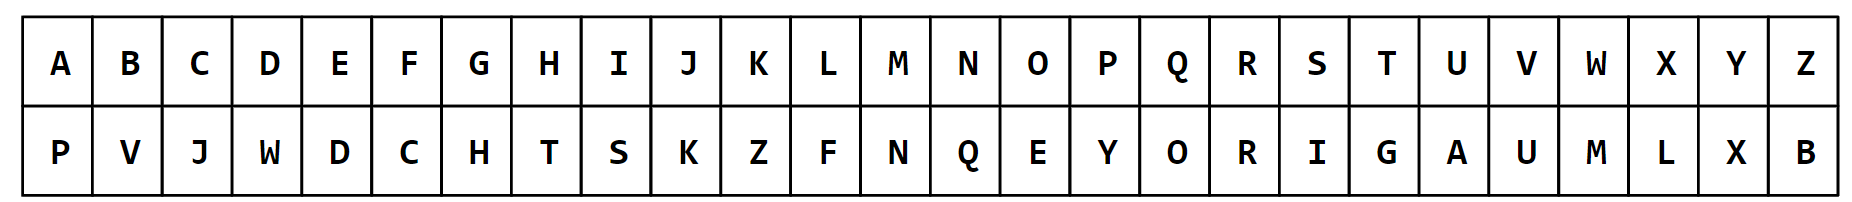
\includegraphics[scale=0.4]{assets/simple_sub.png}
\end{center}
This tells us that 
\begin{itemize}
    \item to \emph{encrypt}, we just need to convert every instance of the top letter to the corresponding bottom letter. For example, encrypting $A$ becomes $P$, encrypting $B$ becomes $V$, and so on.
    \item to \emph{decrypt}, we just need to convert every instance of the bottom letter to the corresponding top letter. For example, decrypting $P$ becomes $A$, decrypting $V$ becomes $B$, and so on.
\end{itemize}
\begin{mdframed}
    (Example.) Suppose Alice wants to encrypt the message \code{You must destroy all of the horcruxes!} She starts by encoding the message\footnote{Removing all spaces, punctuations, and then capitalizing everything.}:
    \begin{verbatim}
YOUMUSTDESTRYALLOFTHEHORCRUXES\end{verbatim}
    Then, she converts each letter using the table: 
    \begin{verbatim}
XEANAIGWDIGREXPFFECGTDTERJRALDI\end{verbatim}
        This is the ciphertext she sends to Bob. To decrypt the message, Bob uses the same table backwards.
\end{mdframed}

Notice that, if the entire table is our key, the number of possible keys is $26!$, a \emph{huge} number. Despite this, simple substitution can still be broken relatively easily using some ideas from probability theory. 

\begin{mdframed}
    (Exercise.) Using the same table given above, do the following by hand. 

    \begin{enumerate}[(a)]
        \item Encrypt the message \code{The moon is pitted with holes!}
        \begin{mdframed}
            Encoding the message gives \code{THEMOONISPITTEDWITHHOLES}. Then, we just need to map each letter appropriately. 
            \begin{verbatim}
plaintext  T H E M O O N I S P I T T E D W I T H H O L E S
ciphertext G T D N E E Q S I Y S G G D W M S G T T E F D I\end{verbatim}
            The answer is \code{GTDNEEQSIYSGGDWMSGTTEFDI}.
        \end{mdframed}

        \item Decrypt the message \code{TEMPRDXEAWESQHGEWPX}.
        \begin{mdframed}
            Mapping each letter appropriately gives us
            \begin{verbatim}
ciphertext T E M P R D X E A W E S Q H G E W P X
plaintext  H O W A R E Y O U D O I N G T O D A Y\end{verbatim}
            Which, decoded, gives us \code{How are you doing today?}
        \end{mdframed}
    \end{enumerate}
\end{mdframed}



\subsection{Polybius Square}
The \textbf{Polybius Square} is another simple substitution cipher which replaces each letter of the plaintext with \emph{two} letters of ciphertext. The idea behind a Polybius square is that it's a table with labeled rows and columns; the alphabet for the messages we're encrypting lives inside the table. For example, if the alphabet we're encrypting includes the capital letters \code{A} through \code{Z} and the digits \code{0} through \code{9}, then we have 36 letters -- perfectly enough to fit in a $6 \times 6$ grid. Consider the following arrangement, using the rows and columns \code{ADFGVX}:
\begin{center}
    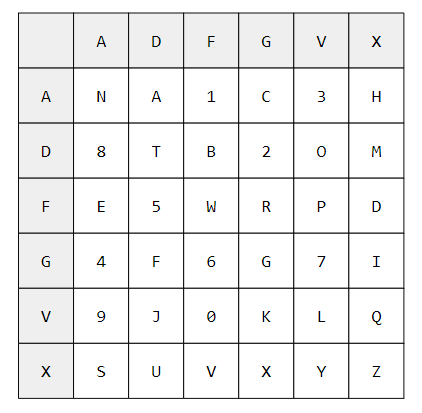
\includegraphics[scale=0.9]{assets/polybius.png}
\end{center}
This table represents our key. To encrypt a message, we convert each letter in the plaintext to a pair of letters indicating the \emph{row} and \emph{column} of that letter in the table above. For example, \code{K} would be replaced with \code{VG}. Similarly, \code{S} would be replaced with \code{XA}. 

\begin{mdframed}
    (Example.) Suppose Alice wants to encrypt the message 
    \begin{verbatim}
Storm the gates at 14:37.\end{verbatim}
    She begins by encoding the message: 
    \begin{verbatim}
STORMTHEGATESAT1437\end{verbatim}
    Then, she goes through and replaces each letter by the corresponding pairs as described above:
    \begin{verbatim}
XADDDVFGDXDDAXFAGGADDDFAXAADDDAFGAAVGV\end{verbatim}
    This is the ciphertext. Bob, who knows the table, can undo this process to decrypt the message. 
\end{mdframed}

\begin{mdframed}
    (Exercise.) Use the square given above.
    \begin{enumerate}[(a)]
        \item Encrypt the message \code{Hide tide at 7:01am}.
        \begin{mdframed}
            Encoding the message gives us \code{HIDETIDEAT701AM}. Then, we can map each individual character in the plaintext to its ciphertext representation:
            \begin{center}
                \begin{tabular}{c|c}
                    \textbf{Plain} & \textbf{Cipher} \\ 
                    \hline 
                    H              & AX \\
                    I              & GX \\
                    G              & GG \\
                    H              & AX \\
                    T              & DD \\
                    I              & GX \\
                    D              & FX \\
                    E              & FA \\
                    A              & AD \\
                    T              & DD \\
                    7              & GV \\
                    0              & VF \\
                    1              & AF \\
                    A              & NN \\
                    M              & DX 
                \end{tabular}
            \end{center}
            Combining all of this gives us 
            \begin{mdframed}
                \begin{verbatim}
AXGXGGAXDDGXFXFAADDDGVVFAFNNDX\end{verbatim}
            \end{mdframed}
        \end{mdframed}
        \item Decrypt the message \code{XAAAADVGFAFVADDDAXADDDDGFVDX}.
        \begin{mdframed}
            To decrypt, we can map each pair of characters in the ciphertext to its plaintext representation:
            \begin{center}
                \begin{tabular}{c|c}
                    \textbf{Cipher} & \textbf{Plain} \\ 
                    \hline 
                    XA              & S \\
                    AA              & N \\
                    AD              & A \\
                    VG              & K \\
                    FA              & E \\
                    FV              & P \\
                    AD              & A \\
                    DD              & T \\
                    AX              & H \\
                    AD              & A \\
                    DD              & T \\
                    DG              & 2 \\
                    FV              & P \\
                    DX              & M 
                \end{tabular} 
            \end{center}
            Combining and decoding gives us 
            \begin{mdframed}
                \begin{verbatim}
Snake path at 2pm\end{verbatim}
            \end{mdframed}
        \end{mdframed}
    \end{enumerate}
\end{mdframed}


\subsection{Interlude: Modular Linear Algebra}
Before going into polygraphic ciphers, let us first discuss how \emph{linear algebra} interacts with modular arithmetic. We'll just work on $2 \times 2$ matrices for now.

\subsubsection{\texorpdfstring{$2 \times 2$ Matrices}{2 by 2 Matrices}}

\begin{definition}{}{}
    A $2 \times 2$ integer \textbf{matrix} (or just \emph{matrix} for short) is a $2 \times 2$ box of numbers $A = \begin{bmatrix}
        a & b \\ c & d
    \end{bmatrix}$ where $a, b, c, d \in \Z$. 
    \begin{itemize}
        \item The \textbf{determinant} of $A$ is the integer $\det(A) = ad - bc$. 
        \item The \textbf{identity matrix} is the matrix $I = \begin{bmatrix}
            1 & 0 \\ 0 & 1
        \end{bmatrix}$. 
        \item Suppose $A = \begin{bmatrix}
            a & b \\ c & d
        \end{bmatrix}$ and $B = \begin{bmatrix}
            a' & b' \\ c' & d'
        \end{bmatrix}$ are two matrices. Their product $AB$ is defined to be \[AB = \begin{bmatrix}
            aa' + bc' & ba' + db' \\ ca' + dc' & cb' + dd'
        \end{bmatrix}.\]
    \end{itemize}
\end{definition}

\begin{mdframed}
    (Example.) Let $A = \begin{bmatrix}
        3 & 2 \\ 1 & 7
    \end{bmatrix}$ and $B = \begin{bmatrix}
        1 & 4 \\ 2 & 3
    \end{bmatrix}$. We know that \[\det(A) = 3 \cdot 7 - 2 \cdot 1 = 19.\] We also know that \[AB = \begin{bmatrix}
        7 & 18 \\ 15 & 25
    \end{bmatrix}\] and \[BA = \begin{bmatrix}
        7 & 30 \\ 9 & 25
    \end{bmatrix}.\] 
\end{mdframed}
\textbf{Remark:} It should be clear from the above example that $AB \neq BA$. That is, matrix multiplication is not commutative. 

\begin{mdframed}
    (Exercise.) Let $A$ be a $2 \times 2$ integer matrix. Show that \[AI = IA = A.\]

    \begin{mdframed}
        Let $A = \begin{bmatrix}
            a & b \\ 
            c & d
        \end{bmatrix}.$ Then, 
        \[IA = \begin{bmatrix}
            1 & 0 \\ 
            0 & 1
        \end{bmatrix} \begin{bmatrix}
            a & b \\ 
            c & d
        \end{bmatrix} = \begin{bmatrix}
            a & b \\ 
            c & d
        \end{bmatrix}\]
        and 
        \[AI = \begin{bmatrix}
            a & b \\ 
            c & d
        \end{bmatrix} \begin{bmatrix}
            1 & 0 \\ 
            0 & 1
        \end{bmatrix} = \begin{bmatrix}
            a & b \\ 
            c & d
        \end{bmatrix}.\]
    \end{mdframed}
\end{mdframed}

\begin{theorem}{Multiplicativity of Determinant}{}
    If $A$ and $B$ are matrices, then $\det(I) = 1$ and \[\det(AB) = \det(A)\det(B).\]
\end{theorem}

\begin{definition}{}{}
    A \textbf{vector} $v$ is a vertical column \[v = \begin{bmatrix}
        x \\ y
    \end{bmatrix},\] where $x, y \in \Z$. 
\end{definition}

\begin{definition}{}{}
    If $A = \begin{bmatrix}
        a & b \\ c & d
    \end{bmatrix}$ is a matrix, then the product $Ab = \begin{bmatrix}
        ax + by \\ 
        cx + dy
    \end{bmatrix}$.
\end{definition}

\subsubsection{Congruences and Inversion for Matrices}
\begin{definition}{}{}
    Fix a positive integer $n$ and suppose $A$ and $B$ are both matrices: 
    \[A = \begin{bmatrix}
        a & b \\ c & d
    \end{bmatrix}, \quad B = \begin{bmatrix}
        a' & b' \\ c' & d'
    \end{bmatrix}.\] We say that $A \equiv B \Mod{n}$ if all four of the entries of the two matrices are congruent mod $n$, i.e., if all of the following are true:  
    \[a \equiv a' \Mod{n}\] 
    \[b \equiv b' \Mod{n}\] 
    \[c \equiv c' \Mod{n}\]
    \[d \equiv d' \Mod{n}\]
\end{definition}

\begin{definition}{}{}
    A matrix $A$ is \emph{invertible mod} $n$ if there exists a matrix $X$ such that $AX \equiv I \Mod{n}$. In this case, $X$ is called an inverse of $A \Mod{n}$. In symbols, we write $X \equiv A^{-1} \Mod{n}$. 
\end{definition}

\begin{theorem}{Modular Inversion Theorem}{}
    Suppose $A = \begin{bmatrix}
        a & b \\ c & d
    \end{bmatrix}$ is a matrix. Then, $A$ is invertible if and only if $\det(A)$ is invertible mod $n$. Moreover, if $e \equiv \det(A)^{-1} \Mod{n}$, then \[X = \begin{bmatrix}
        ed & -eb \\ 
        -ec & ea
    \end{bmatrix}\] is an inverse of $A \Mod{n}$. 
\end{theorem}

\begin{mdframed}
    (Example.) Suppose we have $A = \begin{bmatrix}
        3 & 2 \\ 1 & 7
    \end{bmatrix}$. We know that $\det(A) = 19$ is invertible mod 26, so $A$ is also invertible mod 26. We have \[19^{-1} \equiv 11 \Mod{26},\] so the formula for the inverse from the Matrix Inversion Theorem tells us that \[A^{-1} \equiv \begin{bmatrix}
        11 \cdot 7 & -11 \cdot 2 \\ -11 \cdot 1 & 11 \cdot 3 
    \end{bmatrix} \equiv \begin{bmatrix}
        77 & -22 \\ -11 & 33
    \end{bmatrix} \equiv \begin{bmatrix}
        25 & 4 \\ 15 & 7
    \end{bmatrix} \Mod{26}.\] In other words, \[X = \begin{bmatrix}
        15 & 4 \\ 15 & 7
    \end{bmatrix}\] is an inverse of $A$ mod 26. It follows that $AX = I$. 
\end{mdframed}

\begin{mdframed}
    (Exercise.) Which of the following matrices is invertible mod 26? 
    \begin{enumerate}[(a)]
        \item $\begin{bmatrix}
            7 & 5 \\ 3 & 3 
        \end{bmatrix}$
        \item $\begin{bmatrix}
            8 & 1 \\ 3 & 2 
        \end{bmatrix}$
        \item $\begin{bmatrix}
            4 & 2 \\ 1 & 2 
        \end{bmatrix}$
        \item $\begin{bmatrix}
            4 & 3 \\ 1 & 2
        \end{bmatrix}$
    \end{enumerate}

    \begin{mdframed}
        The answer is \textbf{D}. By calculating the determinant of each matrix, we see that the GCD of the determinant of the matrix and 26 is 1 for only D. 
    \end{mdframed}
\end{mdframed}

\begin{mdframed}
    (Exercise.) As a follow-up to the previous exercise, what is the inverse of the invertible matrix? 

    \begin{mdframed}
        TODO 
    \end{mdframed}
\end{mdframed}

\subsection{Hill Cipher}
The \emph{Hill Cipher} is the first polygraphic cipher we'll talk about. We'll focus on the digraphic case, which replaces 2 letters of plaintext at a time. Our \textbf{key} for this cipher is a matrix that is invertible mod 26. 

\begin{mdframed}
    (Example.) Suppose we want to encrypt the message \textbf{\code{You have saved us all}}. Begin with the usual encoding process: 
    \begin{mdframed}
        \begin{verbatim}
 Y  O  U  H  A  V  E  S  A  V  E  D  U  S  A  L  L
24 14 20  7  0 21  4 18  0 21  4  3 20 18  0 11 11\end{verbatim}
    \end{mdframed} 
    (The numbers below the letters represent the ranking of each letter.) Let's suppose our key is \[A = \begin{bmatrix}
        3 & 2 \\ 1 & 7
    \end{bmatrix},\] which has determinant 19 and is thus invertible mod 26. It follows that $A$ is an invertible matrix mod 26, which can thus be used as a key. 

    \bigskip 

    For encrypting, the idea is to go through the list of numbers, replacing each pair of numbers with the result of multiplying that pair by the matrix $A \Mod{26}$. For example, for the pair 24 and 14, we can make a vector containing these numbers, \[v = \begin{bmatrix}
        24 \\ 14
    \end{bmatrix},\] and then compute \[Av = \begin{bmatrix}
        3 & 2 \\ 1 & 7
    \end{bmatrix} \begin{bmatrix}
        24 \\ 14
    \end{bmatrix} \Mod{26} = \begin{bmatrix}
        100 \\ 122
    \end{bmatrix} \Mod{26} = \begin{bmatrix}
        22 \\ 18
    \end{bmatrix}.\]
    So, we replace the numbers 24 and 14 with the numbers 22 and 18, respectively. In other words, the first two letters of the message will be replaced by \code{W} and \code{S}, respectively. 

    \bigskip 

    We can continue this process with the next pair of numbers (20, 7), and so on. Eventually, we'll reach the end. Note that, if you have an odd number of letters, you can add an additional random letter at the end (e.g., \code{Z}). With this in mind, the net result is the ciphertext
    \begin{mdframed}
\begin{verbatim}
WSWRQRWAQRSZSQWZFE\end{verbatim}
    \end{mdframed}

    As you might expect, to decrypt a message, we just need to multiply the pairs of numbers by the \emph{inverse} of $A$ mod 26.
\end{mdframed}

\begin{mdframed}
    (Exercise.) Use the matrix \[A = \begin{bmatrix}
        3 & -1 \\ 2 & 5
    \end{bmatrix}\] as the key for a Hill cipher. Encrypt the message \code{Go to Lake Lerna}.

    \begin{mdframed}
        First, we verify that this matrix can be used as a key by checking the determinant.
        \[\det(A) = 15 - 2(-1) = 15 + 2 = 17.\]
        Because 17 is invertible mod 26, it follows that we can use $A$ as a key. So, begin by encoding the message: 
        \begin{mdframed}
            \begin{verbatim}
G  O  T  O  L A  K E  L E  R  N A  Z
6 14 19 14 11 0 10 4 11 4 17 13 0 25\end{verbatim}
        \end{mdframed}
        Note that we put a \code{Z} at the end so that the length of the plaintext is even (that way, we can do pairwise encryption.) We'll now process each pair of letters. 
        \begin{itemize}
            \item For pair $(6, 14)$, we have 
            \[\begin{bmatrix}
                3 & -1 \\ 2 & 5
            \end{bmatrix} \begin{bmatrix}
                6 \\ 14
            \end{bmatrix} \Mod{26} = \begin{bmatrix}
                4 \\ 82 
            \end{bmatrix} \Mod{26} = \begin{bmatrix}
                4 \\ 4
            \end{bmatrix},\]
            which corrsponds to \code{E} and \code{E}.

            \item For pair $(19, 14)$, we have 
            \[\begin{bmatrix}
                3 & -1 \\ 2 & 5
            \end{bmatrix} \begin{bmatrix}
                19 \\ 14
            \end{bmatrix} \Mod{26} = \begin{bmatrix}
                43 \\ 108
            \end{bmatrix} \Mod{26} = \begin{bmatrix}
                17 \\ 4
            \end{bmatrix} \Mod{26},\]
            which corresponds to \code{R} and \code{E}.

            \item For pair $(11, 0)$, we have 
            \[\begin{bmatrix}
                3 & -1 \\ 2 & 5
            \end{bmatrix} \begin{bmatrix}
                11 \\ 0
            \end{bmatrix} \Mod{26} = \begin{bmatrix}
                33 \\ 22
            \end{bmatrix} \Mod{26} = \begin{bmatrix}
                7 \\ 22
            \end{bmatrix} \Mod{26},\]
            corresponding to \code{H} and \code{W}.
        \end{itemize}
        By continuing this process, we end up with the ciphertext 
        \begin{mdframed}
\begin{verbatim}
EEREHWAODQMVBV\end{verbatim}
        \end{mdframed}
    \end{mdframed}
\end{mdframed}

\begin{mdframed}
    (Exercise.) Use the matrix \[A = \begin{bmatrix}
        3 & -1 \\ 2 & 5
    \end{bmatrix}\] as the key for a Hill cipher. Decrypt the message \code{RNCQYVFRRLZI}.

    \begin{mdframed}
        Note again that $\det(A) = 17$. In order to decrypt the message, we need to find the inverse of $A$ mod 26.

        \bigskip 

        \textbf{Finding GCD:} Recall that the Matrix Inversion Theorem states that $A$ is invertible if and only if $\det(A)$ is invertible mod $n$. To see if $\det(A)$ is invertible mod $n$, we need to see if $\gcd(\det(A), n) = 1$. So, let's find $\gcd(17, 26)$.  
        \begin{center}
            \begin{tabular}{c|c|c|c|c}
                $a$ & $b$ & $b = aq + r$ & $q$ & $r$ \\ 
                \hline 
                17 & 26 & $26 = 17q + r$ & 1 & 9 \\ 
                9 & 17 & $17 = 9q + r$ & 1 & 8 \\ 
                8 & 9 & $9 = 8q + r$ & 1 & 1 \\ 
                1 & 8 & $8 = 1q + r$ & 8 & 0
            \end{tabular}
        \end{center}
        Therefore, $\gcd(17, 26) = 1$ as desired. Thus, an inverse must exist. 

        \bigskip 
        
        \textbf{Finding Bezout:} Now, we need to find the Bezout coefficients. Labeling each equation, we have 
        \begin{itemize}
            \item (Eq. 1) $26 = 17(1) + 9 \implies 9 = 26 + 17(-1)$ 
            \item (Eq. 2) $17 = 9(1) + 8 \implies 8 = 17 + 9(-1)$
            \item (Eq. 3) $9 = 8(1) + 1 \implies 1 = 9 + 8(-1)$ 
        \end{itemize}
        Now that we've labeled each relevant operation, we can find the Bezout coefficients: 
        \begin{equation*}
            \begin{aligned}
                1 &= 9 + 8(-1) \\ 
                    &= 9 + (\underbrace{17 + 9(-1)}_{\text{Eq. 2}})(-1) \\ 
                    &= 9 + 17(-1) + 9(-1)(-1) \\ 
                    &= 9 + 17(-1) + 9 \\ 
                    &= 9(2) + 17(-1) \\ 
                    &= (\underbrace{26 + 17(-1)}_{\text{Eq. 1}})(2) + 17(-1) \\ 
                    &= 26(2) + 17(-1)(2) + 17(-1) \\ 
                    &= 26(2) + 17(-2) + 17(-1) \\ 
                    &= 26(2) + 17(-3)
            \end{aligned}
        \end{equation*}
        From this, it follows that $x = -3$, which is the desired inverse.  

        \bigskip 

        \textbf{Decrypting:} With this in mind, we have 
        \[X = \begin{bmatrix}
            -3(5) & 3(-1) \\ 3(2) & -3(3)
        \end{bmatrix} = \begin{bmatrix}
            -15 & -3 \\ 6 & -9
        \end{bmatrix} \Mod{26}.\]
        Now that we have the matrix needed to decrypt the message, we can proceed. Labeling each character in the message gives us 
        \begin{mdframed}
            \begin{verbatim}
R  N C  Q  Y  V F  R  R  L  Z I
17 13 2 16 24 21 5 17 17 11 25 8\end{verbatim}
        \end{mdframed}
    \end{mdframed}

    % a pretty stupid hack but at least the frames are readable like this
    \begin{mdframed}
        Iterating over each pair, we have 
        \begin{itemize}
            \item For $(17, 13)$, 
            \[X\begin{bmatrix}
                17 \\ 13
            \end{bmatrix} \Mod{26} = \begin{bmatrix}
                -294 \\ -15
            \end{bmatrix} \Mod{26} = \begin{bmatrix}
                18 \\ 11
            \end{bmatrix} \Mod{26},\]
            or \code{S} and \code{L}. 

            \item For $(2, 16)$, 
            \[X\begin{bmatrix}
                2 \\ 16
            \end{bmatrix} \Mod{26} = \begin{bmatrix}
                -78 \\ -132
            \end{bmatrix} \Mod{26} = \begin{bmatrix}
                0 \\ 24
            \end{bmatrix} \Mod{26},\]
            or \code{A} and \code{Y}.
        \end{itemize}
        By continuing this process, we end up with 
        \begin{mdframed}
            \begin{verbatim}
SLAYTHEHYDRA\end{verbatim}
        \end{mdframed}
    \end{mdframed}
\end{mdframed}

\begin{mdframed}
    (Exercise.) Use the Hill cipher with key \[A = \begin{bmatrix}
        4 & 3 \\ 1 & 2
    \end{bmatrix}\] to encrypt the word \code{AREA}. 

    \begin{mdframed}
        Labeling each letter with its corresponding number, we have 
        \begin{mdframed}
            \begin{verbatim}
0 17 4 0
A  R E A\end{verbatim}
        \end{mdframed}
        Then, we just need to multiply each pair of numbers, like so: 
        \[\begin{bmatrix}
            4 & 3 \\ 1 & 2
        \end{bmatrix} \begin{bmatrix}
            0 \\ 17
        \end{bmatrix} = \begin{bmatrix}
            4 \cdot 0 + 3 \cdot 17 \\ 
            1 \cdot 0 + 2 \cdot 17
        \end{bmatrix} = \begin{bmatrix}
            51 \\ 
            34 
        \end{bmatrix} \equiv \begin{bmatrix}
            25 \\ 
            8
        \end{bmatrix} \Mod{26},\]
        and 
        \[\begin{bmatrix}
            4 & 3 \\ 1 & 2 
        \end{bmatrix} \begin{bmatrix}
            4 \\ 0
        \end{bmatrix} = \begin{bmatrix}
            16 + 0 \\ 
            4 + 0
        \end{bmatrix} \equiv \begin{bmatrix}
            16 \\ 4
        \end{bmatrix} \Mod{26}.\] Therefore, the answer is \code{ZIQE}.
    \end{mdframed}
\end{mdframed}

\begin{mdframed}
    (Exercise.) The matrix \[A = \begin{bmatrix}
        4 & 3 \\ 1 & 2
    \end{bmatrix}\] is used to encrypt \code{CRZX}. What is the plaintext? 

    \begin{mdframed}
        We know that the inverse of $A$ is \[X =  \begin{bmatrix}
            16 & 15 \\ 
            5 & 6 
        \end{bmatrix}.\] Then, going through each pair of numbers gives us 
        \[\begin{bmatrix}
            16 & 15 \\ 5 & 6
        \end{bmatrix} \begin{bmatrix}
            2 \\ 17
        \end{bmatrix} = \begin{bmatrix}
            16 \cdot 2 + 15 \cdot 17 \\ 
            5 \cdot 2 + 6 \cdot 17
        \end{bmatrix} = \begin{bmatrix}
            287 \\ 
            112
        \end{bmatrix} = \begin{bmatrix}
            1 \\ 
            8
        \end{bmatrix},\]
        and 
        \[\begin{bmatrix}
            16 & 15 \\ 5 & 6
        \end{bmatrix} \begin{bmatrix}
            25 \\ 23
        \end{bmatrix} = \begin{bmatrix}
            16 \cdot 25 + 15 \cdot 23 \\ 
            5 \cdot 25 + 6 \cdot 23 
        \end{bmatrix} = \begin{bmatrix}
            745 \\ 263
        \end{bmatrix} \equiv \begin{bmatrix}
            17 \\ 3
        \end{bmatrix}.\]
        This gives us \code{BIRD}.
    \end{mdframed}
\end{mdframed}

\begin{mdframed}
    (Exercise.) Suppose you want to encrypt a sequence of bits (i.e., a sequence of \code{0}'s and \code{1}'s) using a $2 \times 2$ Hill cipher. How many different encryption functions are there? In other words, how many different congruence classes of $2 \times 2$ can be used as a key for a Hill cipher? 

    \begin{mdframed}
        If we assume that our alphabet contains only binary numbers, then there are 2 possible numbers. Therefore, our Hill cipher must be a matrix mod 2. We want to know how many of these matrices are invertible mod 2. 

        \bigskip 

        There are $2 \cdot 2 \cdot 2 \cdot 2$ choices for what our $2 \times 2$ matrix can be. There are three possible determinants: $0$ and $\pm 1$. Note that $-1 \equiv 1 \Mod{2}$ so there's actually \emph{2} possible determinants. Of these determinants, note that $\gcd(1, 2) = 1$ while $\gcd(0, 2) = 2$.
        
        \bigskip 

        With this in mind, we know that any matrix with determinant 1 is valid. There are \boxed{6} such matrices.
    \end{mdframed}
\end{mdframed}

\subsection{Playfair Cipher}
The \textbf{Playfair Cipher} is another digraphic cipher, like the Hill cipher we just discussed above. The key for a Playfair cipher is a $5 \times 5$ grid of letters, where each letter appears exactly once. Because there are 26 letters in the English alphabet but 25 letters can fit in a grid, we treat \code{I} and \code{J} as the same letter\footnote{We could also use a variant where we use a $6 \times 6$ grid that includes all 26 letters and 10 digits, instead.}. 

\bigskip 

How do we start constructing a grid? An easy and convenient way of doing this is to start with a secret keyword. For example, suppose \code{ALPHABET} is our keyword. We can start filling out our grid by writing out the letters of our keyword across the rows, skipping over the letters we've written.
\begin{center}
    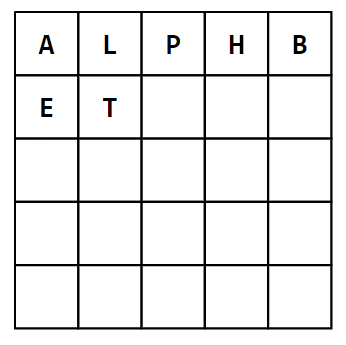
\includegraphics[scale=0.5]{assets/playfair_1.png}
\end{center}
We can then fill out the remaining squares with the remaining letters of the alphabet, skipping over anything we've already written down and remembering that \code{I} and \code{J} are the same. 
\begin{center}
    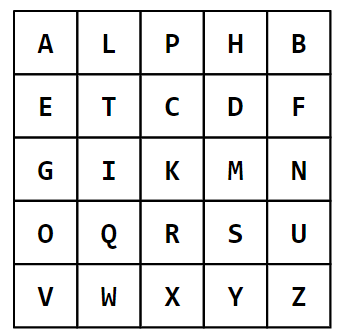
\includegraphics[scale=0.5]{assets/playfair_2.png}
\end{center}
We can encode our message by doing the following: 
\begin{enumerate}
    \item Remove all non-alphabet characters and capitalize everything.
    \item Replace all instances of \code{J} with \code{I}. 
    \item Group the letters into pairs. 
    \item If there are any pairs where both letters are the same, insert the letter \code{X} in between the two letters of that pair and regroup into pairs. 
    \item If there's an unpaired letter at the end, insert the letter \code{X} after it.
\end{enumerate}
\textbf{Remark:} You may need to apply rule 4 multiple times. 

\begin{mdframed}
    (Example.) Suppose we want to encode the message \code{hidden jewels in trees.} Here's what will happen after each step described above. 
    \begin{enumerate}
        \item \code{HIDDENJEWELSINTHETREES}
        \item \code{HIDDENIEWELSINTHETREES}
        \item \code{HI DD EN IE WE LS IN TH ET RE ES}
        \item \code{HI DX DE NI EW EL SI NT HE TR EX ES}
        \item \code{HI DX DE NI EW EL SI NT HE TR EX ES}
    \end{enumerate}
\end{mdframed}

To encrypt, we need to replace each pair with another pair using the grid by following the rules: 
\begin{itemize}
    \item (Row Rule.) If both letters in the pair occur in the same row, replace each letter of the pair with the letter that appears immediately to its right (wrapping around to the left side of the row if needed).
    \item (Column Rule.) If both letters in the pair occur in the same column, replace each letter of the pair with the letter that appears immediately below it (wrapping around to the top of the column if needed).
    \item (Rectangle Rule.) Otherwise, the two letters define a rectangle inside the grid, and we replace each letter with the letter on the same row but the opposite of that rectangle.
\end{itemize}

\begin{mdframed}
    (Example.) Suppose we want to encrypt the message \code{HI DX DE NI EW EL SI NT HE TR EX ES} (see previous example for encoding). Let's look at each pair. 
    \begin{itemize}
        \item For \code{HI}, notice that \code{H} and \code{I} do not appear in the same row or column. Therefore, the rectangle rule applies. Observe the highlighted cells: 
        \begin{center}
            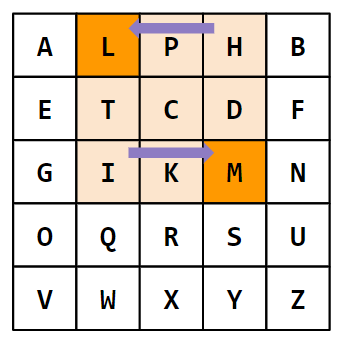
\includegraphics[scale=0.5]{assets/playfair_3.png}
        \end{center}
        Here, the letter in the same row as \code{H} but opposite side is \code{L}, and the letter in the same row as \code{I} but the opposite side is \code{M}. Therefore, \code{HI} becomes \code{LM}. 


        \item For \code{DX}, we also apply the rectangle rule. Observe the highlighted cells: 
        \begin{center}
            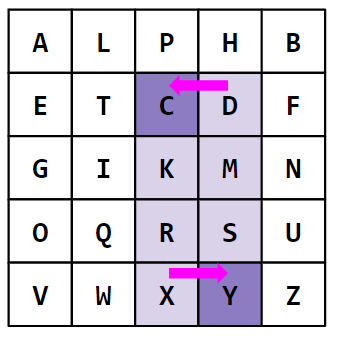
\includegraphics[scale=0.5]{assets/playfair_4.png}
        \end{center}
        So, it follows that \code{DX} gets replaced with \code{CY}.

        \item For \code{DE}, both letters are on the same row so we apply the row rule. Observe that 
        \begin{center}
            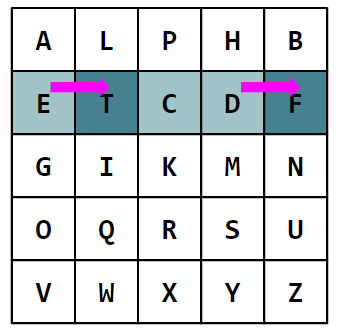
\includegraphics[scale=0.5]{assets/playfair_5.png}
        \end{center}
        So, it follows that \code{DE} becomes \code{FT}.
    \end{itemize}
    Continuing this process yields the desired result.
\end{mdframed}

\begin{mdframed}
    (Exercise.) You are constructing a $5 \times 5$ grid for a Playfair cipher starting with the keyword \code{FAJITAS}. What letter falls in the very center of the grid (i.e., in the 3rd row and the 3rd column)? 

    \begin{enumerate}[(a)]
        \item K
        \item L
        \item M
        \item None of the above. 
    \end{enumerate}

    \begin{mdframed}
        Constructing the grid looks something like: 
        \begin{center}
            \begin{tabular}{|c|c|c|c|c|}
                \hline 
                F & A & I & T & S \\
                \hline 
                B & C & D & E & G \\
                \hline 
                H & K & L & M & N \\
                \hline 
                O & P & Q & R & U \\
                \hline 
                V & W & X & Y & Z \\ 
                \hline 
            \end{tabular}
        \end{center}
        So, the answer is (b). 
    \end{mdframed}
\end{mdframed}

\begin{mdframed}
    (Exercise.) Encode the message \code{Little Fluffy} for encryption using a Playfair cipher. How many pairs of letters are in the encoded message? 

    \begin{enumerate}[(a)]
        \item 6
        \item 7
        \item 8
        \item None of the above. 
    \end{enumerate}

    \begin{mdframed}
        Encoding gives us 
        \begin{itemize}
            \item LITTLEFLUFFY
            \item LITTLEFLUFFY
            \item LITXTLEFLUFXFY
            \item LI TX TL EF LU FX FY
        \end{itemize}
        The answer is (b). 
    \end{mdframed}
\end{mdframed}

\begin{mdframed}
    (Exercise.) Use a Playfair cipher with a key given by the grid below, decrypt \code{WZ LT OP WK SH ES VX PH}.
    \begin{center}
        \begin{tabular}{|c|c|c|c|c|}
            \hline
            C & W & F & Q & Y \\ 
            \hline
            G & I & Z & R & B \\ 
            \hline
            H & M & K & L & U \\ 
            \hline
            V & A & D & E & N \\ 
            \hline
            O & P & X & T & S \\ 
            \hline
        \end{tabular}
    \end{center}

    \begin{mdframed}
        For decryption, we just perform the inverse of the encryption process (e.g., for the row rule, when encrypting is replacing the letter with the one immediately to the right, decrypting is replacing the letter with the one immediately to the left.)
        \begin{itemize}
            \item \code{WZ} maps to \code{FI}.
            \item \code{LT} maps to \code{RE}.
            \item \code{OP} maps to \code{SO}.
            \item \code{WK} maps to \code{FM}.
            \item \code{SH} maps to \code{OU}.
            \item \code{ES} maps to \code{NT}.
            \item \code{VX} maps to \code{DO}.
            \item \code{PH} maps to \code{OM}.
        \end{itemize}
        The answer is \code{FIRESOFMOUNTDOOM}, or \code{Fires of Mount Doom}.
    \end{mdframed}
\end{mdframed}


\subsection{Vigenere Cipher}
The Vigenere cipher is our first example of a \emph{polyalphabetic substitution}, or a substitution cipher in which the substitution scheme changes over the course of the message.

\bigskip 

More specifically, the Vigenere cipher makes use of \emph{modular arithmetic} and the correspondence between the letters \code{A} through \code{Z} and the numbers \code{0} through \code{25}. The \textbf{key} for a Vigenere cipher is a \emph{finite} sequence of shifts. 

\bigskip 

A convenient and, perhaps easy-to-remember, way of constructing such a sequence is to have a secret \emph{keyword}, and then associate each letter of that word with the corresponding number to get the sequence of shift. For example, if our secret keyword is \code{ASGARD}, the corresponding sequence of numbers is $(0, 18, 6, 0, 17, 3)$ because \code{A} corresponds to \code{0}, \code{S} corresponds to \code{18}, and so on.

\begin{mdframed}
    (Example.) Suppose we want to encrypt the message \code{Keep Loki Away}. We begin by encoding the message through the usual way: remove all non-alphabet characters and capitalize everything. 
    \begin{mdframed}
        \code{KEEPLOKIAWAY}
    \end{mdframed}
    Then, we can associate, to each letter in the encoded message, the corresponding numbers 0 through 25.
    \begin{mdframed}
\begin{verbatim}
 K E E  P  L  O  K I A  W A  Y
10 4 4 15 11 14 10 8 0 22 0 24\end{verbatim}
    \end{mdframed}
    We can then perform addition mod 26 to each of these numbers. Specifically, we use the first element of our key sequence for the first number, the second for the second, and so on. When we finish the key, we can just repeat it from the beginning until we're done. From there, we convert those sums back to numbers using te usual correspondence. So, using the key $(0, 18, 6, 0, 17, 3)$ corresponding to the key \code{ASGARD} from above, we have 
    \begin{center}
        \begin{tabular}{c|c c c c c c c c c c c c}
            \textbf{Encoded} & K & E & E & P & L & O & K & I & A & W & A & Y \\ 
            \textbf{Numbers (1)} & 10 & 4 & 4 & 15 & 11 & 14 & 10 & 8 & 0 & 22 & 0 & 24 \\ 
            \textbf{Keyword} & A & S & G & A & R & D & A & S & G & A & R & D \\ 
            \textbf{Key Number (2)} & 0 & 18 & 6 & 0 & 17 & 3 & 0 & 18 & 6 & 0 & 17 & 3 \\ 
            \textbf{(1) + (2) mod 26} & 10 & 22 & 10 & 15 & 2 & 17 & 10 & 0 & 6 & 22 & 17 & 1 \\ 
            \textbf{Encrypted} & K & W & K & P & C & R & K & A & G & W & R & B
        \end{tabular}
    \end{center}
    From this, it follows that \code{KWKPCRKAGWRB} is the ciphertext.
\end{mdframed}
\textbf{Remarks:}
\begin{itemize}
    \item As mentioned earlier, the Vigenere cipher is polyalphabetic. Notice how the first \code{E} in the example above was encrypted to \code{W}, whilethe second \code{E} was encrypted to \code{K}. 
    \item For decryption, the process is nearly the same. The only difference is that we \emph{subtract} mod 26 instead of add. 
\end{itemize} 

\begin{mdframed}
    (Exercise.) Using the keyword \code{ASGARD}, 
    \begin{itemize}
        \item Encrypt the message \code{Protect Odin from Fenrir}.
        \begin{mdframed}
            Encoding the message gives us \code{PROTECTODINFROMFENRIR}. From there, we can label each letter:
            \begin{mdframed}
                \begin{verbatim}
 P  R  O  T E C  T  O D I  N F  R  O  M F E  N  R I  R
15 17 14 19 4 2 19 14 3 8 13 5 17 14 12 5 4 13 17 8 17\end{verbatim}
            \end{mdframed}
            Noting that the key, \code{ASGARD}, has numerical correspondence $(0, 18, 6, 0, 17, 3)$, we can run through the encryption process: 
            \begin{mdframed}
\begin{verbatim}
Encoded            P  R  O  T  E  C  T  O  D  I  N
Numbers (1)        15 17 14 19 4  2  19 14 3  8  13 
Keyword            A  S  G  A  R  D  A  S  G  A  R
Key Numbers (2)    0  18 6  0  17 3  0  18 6  0  17
(1) + (2) mod 26   15 9  20 19 21 5  19 6  9  8  4
Encrypted          P  J  U  T  V  F  T  G  J  I  E

Encoded            F  R  O  M  F  E  N  R  I  R
Numbers (1)        5  17 14 12 5  4  13 17 8  17
Keyword            D  A  S  G  A  R  D  A  S  G
Key Numbers (2)    3  0  18 6  0  17 3  0  18 6
(1) + (2) mod 26   8  17 6  18 5  21 16 17 0  23
Encrypted          I  R  G  S  F  V  Q  R  A  X\end{verbatim}
            \end{mdframed}
            This yields the ciphertext 
            \begin{mdframed}
                \code{PJUTVFTGJIEIRGSFVQRAX}.
            \end{mdframed}
        \end{mdframed}

        \item Decrypt the message \code{RSMNRUOCOSTRMATG}.
        \begin{mdframed}
            We begin by labeling each letter: 
            \begin{mdframed}
                \begin{verbatim}
 R  S  M  N  R  U  O C  O  S  T  R  M A  T G
17 18 12 13 17 20 14 2 14 18 19 17 12 0 19 6\end{verbatim}
            \end{mdframed}
            From there, we can run through the decryption process: 
            \begin{mdframed}
\begin{verbatim}
Encoded            R  S  M  N  R  U  O  C  O  S  T  R  M  A  T  G
Numbers (1)        17 18 12 13 17 20 14 2  14 18 19 17 12 0  19 6
Keyword            A  S  G  A  R  D  A  S  G  A  R  D  A  S  G  A 
Key Numbers (2)    0  18 6  0  17 3  0  18 6  0  17 3  0  18 6  0 
(1) - (2) mod 26   17 0  6  13 0  17 14 10 8  18 2  14 12 8  13 6
Decrypted          R  A  G  N  A  R  O  K  I  S  C  O  M  I  N  G\end{verbatim}
            \end{mdframed}
            Decoding the message yields
            \begin{mdframed}
                \code{Ragnarok is coming} 
            \end{mdframed}
        \end{mdframed}
    \end{itemize}
\end{mdframed}

\begin{mdframed}
    (Exercise.) Use a Vigenere cipher with keyword \code{AND} to encrypt the message \code{Six Meals}. 

    \begin{mdframed}
        Encoding and mapping each letter to the corresponding number, we have 
        \begin{mdframed}
            \begin{verbatim}
S  I  X  M  E  A  L  S
18 8  23 12 4  0  11 18\end{verbatim}
        \end{mdframed}

        From there, we can run through the encryption process: 
        \begin{mdframed}
            \begin{verbatim}
Encoded             S  I  X  M  E  A  L  S
Numbers (1)         18 8  23 12 4  0  11 18
Keyword             A  N  D  A  N  D  A  N
Key Numbers (2)     0  13 3  0  13 3  0  13
(1) + (2) mod 26    18 21 0  12 17 3  11 5
Encrypted           S  V  A  M  R  D  L  F\end{verbatim}
        \end{mdframed}
        Therefore, the answer is \code{SVAMRDLF}.
    \end{mdframed}
\end{mdframed}

\begin{mdframed}
    (Exercise.) Use a Vigenere cipher with keyword \code{AND} to decrypt \code{YEX SUD LYQ OGS AFV}. 

    \begin{mdframed}
        Running through the decryption process yields 
        \begin{mdframed}
\begin{verbatim}
Encoded             Y  E  X  S  U  D  L  Y  Q  O  G  S  A  F  V 
Numbers (1)         24 1  23 18 20 3  11 24 16 14 6  18 0  5  21
Keyword             A  N  D  A  N  D  A  N  D  A  N  D  A  N  D
Key Numbers         0  13 3  0  13 3  0  13 3  0  13 3  0  13 3
(1) - (2) mod 26    24 14 20 18 7  0  11 11 13 14 19 15 0  18 18
Decrypted           Y  O  U  S  H  A  L  L  N  O  T  P  A  S  S 
\end{verbatim}
        \end{mdframed}
        This yields \code{YOUSHALLNOTPASS}, or \code{You shall not pass}.
    \end{mdframed}
\end{mdframed}

\subsection{One-Time Pad}
The \emph{one-time pad} is a special case of the Vigenere cipher where the key sequence is 
\begin{itemize}
    \item never re-used, 
    \item at least as long as the plaintext, 
    \item ``unrelated to the plaintext,'' and 
    \item ``totally random,'' in the sense that each number 0 through 25 is equally likely in each position of the key.
\end{itemize}
Essentially, the way the one-time pad functions is very similar to the Vigenere cipher, except that the key sequence must not be generated using a keyword\footnote{The issue with this is that words won't have the property that each letter is equally likely.}. 

\bigskip 

In any case, we'll revisit this section later -- it's important to be precise when talking about what ``unrelated to the plaintext'' and ``totally random'' means. We'll also see, later on, that this has a property known as \emph{perfect secrecy}, which means that the security of the one-time pad can be mathematically guaranteed. 










\newpage 
\section{Codebreaking}
In the previous section, we mostly looked at encryption and decryption of many ciphers. Now, we'll look at how to \emph{break} some of these ciphers. It should be noted that codebreaking is not necessarily ``exact science''; that is, there's not necessarily an algorithm that guarantees producing the correct plaintext from ciphertext in one shot without access to the key. Instead, these techniques can help constrain the search for the correct ciphertext. 

\subsection{Frequency Analysis}
\textbf{Frequency analysis} is a powerful technique used to break simple -- and sometimes also polygraphic -- substutition ciphers. The idea is relatively simple. 

\begin{displayquote}
    \textbf{Heuristic:} The relative frequencies of letters remain \emph{roughly} stable across different samples of English texts, and \code{ETAOINSHRDLU} is the \emph{approximate} order of the 12 most common letters.
\end{displayquote}

We can use this heuristic to break simple substutition ciphers. Ideally, the technique works best with longer ciphertexts, but the idea is to guess the decryption key one letter at a time, doing one of the following at each step: 
\begin{enumerate}
    \item Assign the most frequent unassigned letter of ciphertext to be the most frequent unassigned letter in some sample English text (or perhaps some other letter with a similar frequency).
    \item Look through the ciphertext and see if you can make any guesses about words that seem to appear there. If you see something, fill in the blanks in that word by making appropriate guesses for the key.
\end{enumerate}
If, at any point, it seems like your guesses are leading to nonsense or implausible sequences of letters, backtrack and make another guess. A few comments: 
\begin{itemize}
    \item Usually, we can start with two applications of option 1. For example, we can guess that the most common letter in the ciphertext is \code{E} and the second most commmon letter is \code{T}. 
    \item We can also note that \code{THE} occurs frequently in English (and other similar words like \code{THEY} or \code{THEIR} or \code{THEN}). 
    \item If, after you make the \code{T} and \code{E} substutitions, you see the \code{T*E} pattern frequently (\code{*} being some \emph{fixed} letter in ciphertext), you can make the assumption that \code{*} could be \code{H}. 
    \begin{itemize}
        \item Also, perhaps if you see \code{TH*T} occurring in your ciphertext after making the substutitions and with \code{*} fixed, you can probably assume that \code{*} is \code{A}. 
    \end{itemize}

    \item If you can't spot any possible words, you can always try using option 1 instead and match the most frequent letters. 
\end{itemize}
Usually, the first few guesses after \code{E} and \code{T} are the hardest. Once you've made a few correct guesses, it becomes easy to see words.

\subsection{Interlude: Probability}
Notice how, in the previous observation, we made use of the Heuristic to help us mount attacks on substutition ciphers. We can use variants of this observation for other ciphers, but this requires us to first talk about \textbf{probability}.

\subsubsection{Experiments and Events}
In probability thoery, the word \emph{experiment} is used to talk abstractly and heuristically about processes which generate ``outcomes'' and which might be rather intricate. These experiments are formally modeled by \emph{probability spaces}. For now, we'll use the following definition. 
\begin{definition}{(Discrete) Probability Space}{}
    A \textbf{(discrete) probability space} is a nonempty countable\footnote{``Countable'' means that the outcomes can be put in a list so that the summation $\sum_{x \in \Omega} \PR[x]$ makes sense. Any finite set, and some infinite sets, are countable. For now, we'll focus on the finite case.} set $\Omega$ called the \textbf{sample space} and whose elements are called \textbf{outcomes}. Each outcome $x \in \Omega$ is assigned a real number $\PR[x]$ between 0 and 1 called its \textbf{probability}. The probabilities of all the outcomes must sum to 1; that is, 
    \[\sum_{x \in \Omega} \PR[x] = 1.\]
\end{definition}
The probability associated to each outcome should be thought of as some measure of our ``confidence'' that our experiment will produce that outcome. For example, it might be the percentage of times we expect the experiment to produce that outcome if the experiment were to be releated many times. 

\begin{mdframed}
    (Example.) Rolling a dice is an example of an experiment. 
    \begin{itemize}
        \item The possible outcomes of this experiment are the numbers 1 through 6; that is, the \textbf{sample space} is \[\Omega = \{1, 2, 3, 4, 5, 6\}.\] 
        \item Assigning each outcome a probability of $\frac{1}{6}$, that is, for $x \in \Omega$, \[\PR[x] = \frac{1}{6},\] means that the dice is ``fair'' and each outcome is equally likely. 
    \end{itemize}
    Thus, we constructed a probability space; we have a finite set $\Omega$ that enumerates the possible outcomes, and we assigned a probability to each outcome. 
\end{mdframed}

A single experiment can also have ``multiple parts,'' as seen in the next example. 
\begin{mdframed}
    (Example.) Flipping a fair coin twice can be thought of as a single experiment. 
    \begin{itemize}
        \item Possible outcomes of this experiment might be something like ``heads and then heads again'' or ``heads and then tails'' and so on. All these outcomes taken together as a set form the sample space, 
        \[\Omega = \{HH, HT, TH, TT\},\]
        where $H$ means ``Heads'' and $T$ means ``Tails.''

        \item We can assign each of these four outcomes probability $\frac{1}{4}$, that is for some $x \in \Omega$
        \[\PR[x] = \frac{1}{4}.\]
    \end{itemize}
    Here, we've modeled the situation where the coin is fair and the result of each coin flip is unrelated to the other. 
\end{mdframed}
Notice how both examples above have outcomes with the same probabilities. This is a common situation, and thus has a name.

\begin{definition}{Uniform Distribution}{}
    A probability space is \textbf{uniform} if all of its outcomes have equal probability. 
\end{definition}
Sometimes, we might be interested in grouping the various outcomes together. We can do so with a definition.

\begin{definition}{Event}{}
    Given a probability space, an \textbf{event} $E$ is a subset of the sample space $\Omega$; that is, 
    \[E \subset \Omega.\]
    We define 
    \[\PR[E] = \sum_{x \in E} \PR[x].\]
\end{definition}
\textbf{Remark:} The words ``event'' and ``outcome'' have distinct definitions in probability theory.

\begin{mdframed}
    (Example.) Consider the example of rolling a dice again. An \emph{event} might be something like ``the dice roll is odd.'' Formally, if we think of the sample space $\Omega = \{1, 2, 3, 4, 5, 6\}$, the event ``the dice roll is odd'' corresponds to the event \[E = \{1, 3, 5\}.\] This event is also assigned a probability, by summing together the probabilities of all outcomes that comprise the event:
    \[\PR[E] = \PR[1] + \PR[3] + \PR[5] = \frac{1}{6} + \frac{1}{6} + \frac{1}{6} = \frac{3}{6} = \frac{1}{2}.\]
\end{mdframed}

\begin{mdframed}
    (Exercise.) Suppose you have 4 boxes (labeled 1, 2, 3, and 4), and you have 8 colors available (red, blue, green, yellow, pink, purple, teal, brown). Consider an experiment where each of the 4 boxes is assigned a color. For example, one possible outcome of this experiment might be the one where box 1 is colored red, box 2 is colored blue, box 3 is colored green, and box 4 is colored blue.

    \begin{enumerate}
        \item How many possible outcomes are there?
        \begin{mdframed}
            The answer is $8^4 = 70$ outcomes. We can assign any of the 8 colors to box 1, any of the 8 colors to box 2, any of the 8 colors to box 3, and any of the 8 colors to box 4.   
        \end{mdframed}
        \item How many outcomes are in the event ``no two boxes have the same color?''
        \begin{mdframed}
            The answer is $8 \cdot 7 \cdot 6 \cdot 5 = 1680$. Once we pick a color, we can no longer use that color for the next box. 
        \end{mdframed}
    \end{enumerate}
\end{mdframed}

\begin{mdframed}
    (Exercise.) Suppose you have $k$ boxes and you have $n$ colors available. Consider again the same experiment where each of the $k$ boxes is assigned one of the $n$ colors ``at random'' (i.e., construct a uniform probability space).
    \begin{enumerate}
        \item What is the probability of the event that no two boxes have the same color? 
        \begin{mdframed}
            Note that the number of outcomes such that no two boxes have the same color is given by $n \cdot (n - 1) \cdot (n - 2) \cdot (n - 3) \cdot \hdots \cdot (n - k + 1)$. The total number of outcomes is $n^k$. The probability is given by \[\frac{n \cdot (n - 1) \cdot (n - 2) \cdot (n - 3) \cdot \hdots \cdot (n - k + 1)}{n^k}.\]
        \end{mdframed}
        \item What is the probability that there are at least two boxes of the same color? 
        \begin{mdframed}
            Note that the event that at least two boxes have the same colors is the opposite of the event that no two boxes have the same colors. In other words, 
            \[\PR(\geq 2\text{ Boxes Have Same Color}) = 1 - \PR(\text{No Two Boxes Have Same Color}).\]
            This gives us 
            \[\PR(\geq 2\text{ Boxes Have Same Color}) = 1 - \frac{n \cdot (n - 1) \cdot (n - 2) \cdot (n - 3) \cdot \hdots \cdot (n - k + 1)}{n^k}.\]
        \end{mdframed}
        \item Find expressions in terms of $n$ and $k$. 
        \begin{mdframed}
            Notice that 
            \[n \cdot (n - 1) \cdot (n - 2) \cdot (n - 3) \cdot \hdots \cdot (n - k + 1) = (n)_k = \frac{n!}{(n - k)!}.\] This is known as a falling factorial. So, 
            \begin{enumerate}
                \item $\frac{\frac{n!}{(n - k)!}}{n^k}$.
                \item $1 - \frac{\frac{n!}{(n - k)!}}{n^k}$.
            \end{enumerate}
        \end{mdframed}
    \end{enumerate}
\end{mdframed}


\subsubsection{Random Variables}
A common way that events show up is through \textbf{random variables}. We can think of random variables as representations of making an observation (or taking a measurement) on the outcome of an experiment. A random variable has a set of possible values that it can take. Letters like $X$ or $Y$ can be used to denote random variables. 
\begin{definition}{Random Variable}{}
    Fix a probability space $\Omega$. A \textbf{random variable} is a function with domain $\Omega$ and its set of \emph{possible} values is the range of this function. 
\end{definition}

\begin{mdframed}
    (Example.) Consider the ``multi-part'' experiment discussed earlier (with the coin being flipped twice). We can make the observation that the first coin flip can be thought of as a random variable, which we can call $X$. $X$ can take the value ``heads'' or ``tails.'' Then, we can write things like $X = H$ to refer to the event that the first coin flip landed heads. In other words, in the sample space \[\Omega = \{HH, HT, TH, TT\},\] the notation $X = H$ describes the event $\{HH, HT\}$ and we have \[\PR[X = H] = \PR[HH] + \PR[HT] = \frac{1}{4} + \frac{1}{4} = \frac{1}{2}.\]
\end{mdframed}

\begin{mdframed}
    (Example.) Suppose we're interested in the number of heads. We can define another random variable $Y$ that can take values 0, 1, or 2. The notation $Y = n$ for either $n = 0, 1, 2$ describes the event that we observe $n$ heads out of the two coin flips. So, for $Y = 1$, we have the event $\{HT, TH\}$ and \[\PR[Y = 1] = \PR[HT] = \PR[TH] = \frac{1}{4} + \frac{1}{4} = \frac{1}{2}.\]
    However, for $Y = 0$, we have the event $\{TT\}$ and \[\PR[Y = 0] = \PR[TT] = \frac{1}{4}.\]
\end{mdframed}

\begin{definition}{Uniform Random Variable}{}
    A random variable is \textbf{uniform} if all of its values have equal probability.
\end{definition}
In the previous two examples, $X$ is uniform (it can either take heads or tails, i.e., $X = H$ or $X = T$, both of which have probabilities $1/2$) whereas $Y$ is not uniform.

\begin{definition}{Expected Value}{}
    Suppose $X$ is a random variable whose values are real numbers. The \textbf{expected value}, known as the expectation, of $X$, denoted $\E[X]$, is defined by \[\E[X] = \sum_{\text{values } a} a \cdot \PR[X = a].\]
\end{definition}

\begin{mdframed}
    (Example.) In the experiment involving two coin flips, the random variable $Y$ which counts the number of heads has real number values (0, 1, 2). Its expectation is given by 
    \[\E[Y] = 0 \cdot \frac{1}{4} + 1 \cdot \frac{1}{2} + 2 \cdot \frac{1}{4} = 1.\]
\end{mdframed}

\begin{mdframed}
    (Exercise.) Consider the experiment where you roll a pair of fair dice. Let the random variable $X$ denote the sum of the dice rolls. 
    \begin{enumerate}
        \item What are the possible values of $X$? 
        \begin{mdframed}
            The possible values are \[\{2, 3, 4, 5, 6, 7, 8, 9, 10, 11, 12\}.\]
        \end{mdframed}
        \item What is $\PR[X = 7]$?
        \begin{mdframed}
            Note that the pair of fair dice will have sum 7 if we get 
            \[\{(1, 6), (2, 5), (3, 4), (4, 3), (5, 2), (6, 1).\}\]
            Therefore, 
            \[\PR[X = 7] = \frac{6}{36} = \frac{1}{6}.\]
        \end{mdframed}
        \item What is $\PR[X = 7 \text{ or } 11]$?
        \begin{mdframed}
            Note that the paur of fair dice will have 11 if we get 
            \[\{(6, 5), (5, 6)\}.\]
            Combining this with this previous part, we have 8 possible combinations. This gives us 
            \[\PR[X = 7 \text{ or } 11] = \frac{8}{36} = \frac{2}{9}.\]
        \end{mdframed}
        \item What is $\E[X]$? 
        \begin{mdframed}
            Note that
            \begin{itemize}
                \item For sum 2, there is only 1 possible combination. 
                \item For sum 3, there are 2 possible combinations.
                \item For sum 4, there are 3 possible combinations.  
                \item For sum 5, there are 4 possible combinations. 
                \item For sum 6, there are 5 possible combinations. 
                \item For sum 7, there are 6 possible combinations. 
                \item For sum 8, there are 5 possible combinations. 
                \item For sum 9, there are 4 possible combinations. 
                \item For sum 10, there are 3 possible combinations. 
                \item For sum 11, there are 2 possible combinations. 
                \item For sum 12, there are 1 possible combinations. 
            \end{itemize}
            Therefore, the expected value is 
            \begin{equation*}
                \begin{aligned}
                    \E[X] &= 2 \frac{1}{36} + 3 \frac{2}{36} + 4 \frac{3}{36} + 5 \frac{4}{36} + 6 \frac{5}{36} + 7 \frac{6}{36} + 8 \frac{5}{36} + 9 \frac{4}{36} + 10 \frac{3}{36} + 11 \frac{2}{36} + 12 \frac{1}{36} \\ 
                        &= 7.
                \end{aligned}
            \end{equation*}
        \end{mdframed}
    \end{enumerate}
\end{mdframed}

\subsection{Interlude: G-Test}
Suppose that every registered voters in an imaginary county in the United States is classified into the mutually exclusive and exhaustive racial groups ``White,'' ``Black,'' ``Hispanic,'' and ``Other.'' Suppose that, by inspecting the voter rolls, we find that the racial distribution of this county is 
\begin{center}
    \begin{tabular}{c|c c c c c}
            & White & Black & Hispanic & Other & Total \\
        \hline  
        Distribution & 72\% & 7\% & 12\% & 9\% & 100\%
    \end{tabular}
\end{center}
Since jurors are supposed to be drawn from the list of registered voters, we might hope that a random sample of jurors would follow this same racial distribution. Suppose we sample 275 jurors and observe the racial distribution displayed in the second row:
\begin{center}
    \begin{tabular}{c|c c c c c}
            & White & Black & Hispanic & Other & Total \\
        \hline  
        Distribution & 72\% & 7\% & 12\% & 9\% & 100\% \\ 
        Observed & 210 & 10 & 20 & 35 & 275 \\ 
        Expected & 198 & 19.25 & 33 & 24.75 & 275
    \end{tabular}
\end{center}
Now, if our random sample of jurors followed the overall racial distribution of registered voters, we would expect that 72\% of them would be White, which would be $0.72 \cdot 275 = 198$ people. We can calculate the expected numbers of jurors in the other groups similarly to fill in the third row above.

\bigskip 

Note that we can, and should, expect \emph{some} deviation from the expected counts. Remembering that our categories are mutually exclusive, so we could not possibly observe a sample of 19.25 Black jurors. However, if we had expected something like 198 White jurors, 19 Black jurors, 33 Hispanic jurors, and 25 Other jurors -- or something close to that -- we probably would not be surprised with our results.

\bigskip 

Stated differently, \emph{the data we collected would feel consistent with the hypothesis that the racial distribution of jurors matches the racial distribution of the electorate.} However, what we observed was pretty far from the expected counts. \textbf{How do we quantify and make sense of this observation?}

\subsubsection{The G-Test}
The idea is to introduce a number that measures the difference between the observed and expected rows. There are a variety of numbers that can be used, but let us consider one that is often denoted $G$. It is defined as follows: 

\begin{definition}{}{}
    Suppose $X$ is a random variable with finitely many values $a_1, \hdots, a_n$ and let $p_i = \PR[X = a_i]$. Suppose we make $N$ observations of the values $a_1, \hdots, a_n$ and that $O_i$ is the number of observations of $a_i$ that we made. Let $E_i = Np_i$ and then define \[G = 2\sum_{i} O_i \ln\left(\frac{O_i}{E_i}\right).\] If $O_i = 0$ for some $i$, we set the corresponding summand $O_i\left(\frac{O_i}{E_i}\right) = 0$. If there exists an $i$ such that $E_i = 0$ but $O_i \neq 0$, set $G = \infty$. 
\end{definition}

\begin{mdframed}
    (Example.) Consider the motivating example with the voters. Define 
    \begin{itemize}
        \item The random variable $X$ represents observing the race of a randomly drawn voter from our county. It has 4 possible values (White, Black, Hispanic, Other), so $n = 4$. 
        
        \item The values $p_i$ are the percentages of the electorate in each racial group. 
        \item The values $O_i$ are the observed counts. 
        
        \item The values $E_i$ are the expected counts. 
        
        \item For fun, $N = 275$ (we have 275 total observations across $a_1, a_2, a_3, a_4$). 
    \end{itemize}
    Then, 
    \[G = 2\left(210 \ln\left(\frac{210}{198}\right) + 10 \ln\left(\frac{10}{19.25}\right) + 20 \ln\left(\frac{20}{33}\right) + 35\ln\left(\frac{35}{24.75}\right)\right) \approx 15.84.\]
\end{mdframed}
\textbf{Remark:} If you're inclined to see why $E_i = Np_i$, note that $N = 275$ (that's the number of observations of all the values) and $p_i$ is the percent of the electorate in the racial group $i$. So, for Black, $E = 275 \cdot 0.07 = 19.25$. 

\bigskip 

\begin{theorem}{Gibbs' Inequality}{}
    We always have $G \geq 0$. Moreover, $G = 0$ if and only if $O_i = E_i$ for all $i = 1, \hdots, n$. 
\end{theorem}
The question is simply, how big is ``big?'' In particular, in our example, can we say 15.84 is a ``\emph{big}'' value of $G$? The answer to this question is provided by the following theorem, which we'll state slightly imprecisely and explain in a bit more detail later. 

\begin{theorem}{Wilks' Theorem}{}
    Suppose the $N$ observations of the values $a_1, \hdots, a_n$ that we make are in fact independent observations of the random variable $X$. For large values of $N$, the values of $G$ are well-approximated by a chi-square distribution with $n - 1$ degrees of freedom.
\end{theorem}
There are several points of explanation to make.
\begin{itemize}
    \item A ``chi-square distribution with $k$ degrees of freedom'' is a certain function $f_k$ defined on $[0, \infty)$ and taking non-negative values everywhere with total integral equal to 1. In other words, we have $f_{k}(x) \geq 0$ for all $x \geq 0$ and \[\int_{0}^{\infty} f_{k}(x) dx = 1.\] The formula for $f_{k}(x)$ is complicated and also unimportant for our purposes. 
    
    \item To say that ``the values of $G$ are well-approximated by a chi-square distribution with $n - 1$ degrees of freedom'' is to say that, for any (not necessarily finite) interval $(a, b)$, the probability that $G$ lands inside the interval $(a, b)$ is approximately 
    \[\int_{a}^{b} f_{k}(x) dx.\]

    \begin{mdframed}
        (Example.) Notice that 
        \[\int_0^{15.84} f_{3}(x)dx \approx 0.999.\]
        It follows that 
        \[\int_{15.84}^{\infty} f_{3}(x) dx = 1 - \int_{0}^{15.84} f_3(x) \approx 1 - 0.999 = 0.001.\]
        The number 0.001 is our $p$-value, and it means that the probability of observing a value of $G$ that is bigger than 15.84 is only about 0.1\%. That is quite a small probability, so our calculation suggests that the value of $G$ that we saw is in fact quite large. 
    
        \bigskip 
    
        Stated differently, with a $p$-value of 0.001, this indicates that if jurors in this county were truly representative of the county's electorate, there would only be roughly a 0.1\% chance of seeing a sample that deviated at least as much from the expected counts as the data that we saw. Because that's such a small probability, this suggests that it's very unlikely that our sample of jurors is actually representative of the county's electorate. We have quantified the observation we made informally above.
    \end{mdframed}

    \item Another thing to look at is ``for large values of $N$.'' In particular, that this theorem would only work for large values of $N$. Was $N = 275$ large enough to justify what we did? The answer \emph{depends} on how well you want the values of $G$ to be approximated by a chi-square distribution. The better an approximation you want, the higher a value of $N$ you need. That being said, the following heuristic generally works well. 
\end{itemize}

\begin{theorem}{Heuristic Addendum to Wilks' Theorem}{}
    The approximation of $G$ by a chi-square distribution with $n - 1$ degrees of freedom is ``good enough'' as long as the vast majority of the expected counts $E_1, \hdots, E_n$ are all at least 5.
\end{theorem}
Because all of our expected counts are well above 5, we do not need to worry. 

\bigskip 

The process (computing expected counts, finding an observed value of $G$, using a chi-square approximation to find a $p$-value, i.e., the probability of observing a larger value of G than what we observed if the observations do in fact come from the theoretical distribution) is called a \textbf{G-test}. It's a useful technique for a lot of problems in statistics and can be used in codebreaking. 


\begin{mdframed}
    (Exercise.) A professor using an open source introductory statistics book predicts that 60\% of the students will purchase a hard copy of the book, 25\% will print it out from the web, and 15\% will read it online. At the end of the semester she asks her students to complete a survey where they indicate what format of the book they used. Of the 126 students, 71 said they bought a hard copy of the book, 30 said they printed it out from the web, and 25 said they read it online. How well does this data fit the professor's predictions? Run a $G$-test to find out!

    \begin{mdframed}
        Similar to the introduction of this section, we can create a table. 
        \begin{center}
            \begin{tabular}{c|c c c c}
                    & Hard Copy & Web & Online & Total \\
                \hline  
                Distribution & 60\% & 25\% & 15\% \\ 
                Observed & 71 & 30 & 25 & 126 \\ 
                Expected & 75.6 & 31.5 & 18.9 & 126
            \end{tabular}
        \end{center}
        Note that 
        \begin{itemize}
            \item $X$ represents observing whether a person reads from a hard copy, web, or online. Therefore, $n = 3$.
            \item The values $p_i$ represents the percentages that a person chooses to either purchase a hard copy, or print it out, or read it online.
            \item The values $O_i$ are the observed counts. 
            \item The values $E_i$ are the expected counts. 
        \end{itemize}
        
        Calculating the $G$ value, we have 
        \[G = 2\left(71\ln\left(\frac{71}{75.6}\right) + 30\ln\left(\frac{30}{31.5}\right) + 25\ln\left(\frac{25}{18.9}\right)\right) \approx 2.14403.\]
        We now want to see what the probability is of observing a value of $G$ that is bigger than 2.14403. To do this, note that 
        \[\int_{2.14403}^{\infty} f_{2}(x) = 1 - \int_{0}^{2.14403} f_{2}(x) \approx 1 - 0.65768194886549 = 0.342318.\]
        So, $0.342318$ is our $p$-value, and it follows that the probability that we find a higher $G$ value is about $34.23\%$. In other words, there would be a 34.23\% chance of seeing a sample that deviated as least as much from the expected counts as the data we just saw. 
    \end{mdframed}
\end{mdframed}



\subsection{Breaking Rectangular Transposition}
Suppose you're given a long passage of ciphertext (with 2808 characters) that is known to be encrypted using rectangular transposition. How do we break the code? We'll talk about a strategy for breaking the code. 
\begin{enumerate}
    \item First, start by making an arbitrary guess for the ``period,'' i.e., the length of the key word. We know that the period has to be a \emph{divisor} of the length of the ciphertext. Note that 2808 has 32 possible divisors: 
    \[\{1,2,3,4,6,8,9,12,13,18,24,26,27,\hdots,234,312,351,468,702,936,1404,2808\}.\]
    Since there are only 26 characters in the English alphabet, the period can be at most 26. This means that the period must be one of the following: 
    \[\{1,2,3,4,6,8,9,12,13,18,24,26\}.\]
    Suppose we guess that the period is 6.

    \item Next, we can arrange our ciphertext into a rectangle of length 6 (the period we guessed). Note that our rectangle will have height $N = \frac{2808}{6} = 468$, so for the sake of being concise only the first few rows will be shown: 
    \begin{verbatim}
    OIPWMJ
    ALWSLE
    LJLYEA
    MENUAB
    IHSDAC
    ESRTIE
    EMKHAO
    AMNPAI
    IELNAP
       .
       .
       .\end{verbatim}

    \item For every pair of numbers $i \neq j$ between 1 and 6 (the period we guessed), we consider the tall column of width 2 we would get by placing the $i$th and $j$th column of the above rectangle next to each other. For example, if $i = 4$ and $j = 2$, we would get the following $468 \times 2$ rectangle:
    \begin{verbatim}
        WI
        SL
        YJ
        UE
        DH
        TS
        HM
        PM
        NE
        .
        .
        .\end{verbatim}


    \item We can think of this as 468 observations of a pair of English letters \emph{if} the columns $i$ and $j$ were consecutive in the plaintext.In particular, for every pair of letters $\alpha$ and $\beta$, we count the number of times that we see the sequence $\alpha \beta$ appearing in this column. Let $O_{\alpha\beta}^{(i, j)}$ be this number. In our truncated example above (in step 3), notice that $O_{\text{WI}}^{(4, 2)}$, $O_{\text{SL}}^{(4, 2)}$, etc. are all at least 1.
    
    \bigskip 

    On the other hand, we can use a large sample of English to calculate the probability $p_{\alpha\beta}$ of the pair $\alpha\beta$ occurring in the English text. We can use these to calculate the expected counts $E_{\alpha\beta} = Np_{\alpha\beta} = 468p_{\alpha\beta}$ and then calculate a corresponding value of $G$ using the observed counts $O_{\alpha\beta}^{(i, j)}$. We can call this $G^{(i, j)}$; in other words, 
    \[G^{(i, j)} = \sum_{\alpha\beta} O_{\alpha\beta}^{(i, j)} \ln\left(\frac{O_{\alpha\beta}^{(i, j)}}{E_{\alpha\beta}}\right).\]
    We can then assemble all of these values\footnote{Note that all the diagonal entries of this box are set to $\infty$ since we only compute $G^{(i, j)}$ when $i \neq j$. This is an \underline{arbitrary} convention and the diagonal entries should just be ignored.} of $G^{(i, j)}$ as $i \neq j$ varies into a box of numbers: 
    \[\begin{bmatrix}
        \infty     & G^{(1, 2)} & G^{(1, 3)} & G^{(1, 4)} & G^{(1, 5)} & G^{(1, 6)} \\ 
        G^{(2, 1)} & \infty     & G^{(2, 3)} & G^{(2, 4)} & G^{(2, 5)} & G^{(2, 6)} \\ 
        G^{(3, 1)} & G^{(3, 2)} & \infty     & G^{(3, 4)} & G^{(3, 5)} & G^{(3, 6)} \\ 
        G^{(4, 1)} & G^{(4, 2)} & G^{(4, 3)} & \infty     & G^{(4, 5)} & G^{(4, 6)} \\ 
        G^{(5, 1)} & G^{(5, 2)} & G^{(5, 3)} & G^{(5, 4)} & \infty     & G^{(5, 6)} \\ 
        G^{(6, 1)} & G^{(6, 2)} & G^{(6, 3)} & G^{(6, 4)} & G^{(6, 5)} & \infty
    \end{bmatrix}.\]
    If we guessed the period correctly, then we should find that every row except \emph{one of them} has \emph{one} number that's much smaller than all the others. This tells us something about how to permute the letters to find the plaintext. For example, if we find in the first row that $G^{(1, 4)}$ is \emph{much} smaller than the other numbers, that tells us that rows 1 and 4 are likely to be \emph{consecutive} in the plaintext, because the frequency distribution of the pairs that occur in the long $468 \times 2$ rectangle displayed earlier is close to the frequency distribution of pairs that occur in the English plaintext.

    \bigskip 

    Note that there are \emph{many} calculations to do by hand. Therefore, we will make use of a compute to do these calculations for us. 
\end{enumerate}

\begin{mdframed}
    (Example.) Suppose our ``$G$-box'' is 
    \[\begin{bmatrix}
        \infty & 1151.3 & 1090.2 & \underline{\textbf{485.5}} & 1069.3 & 1005.0 \\ 
        1234.4 & \infty & 1228.3 & 1049.6 & \underline{\textbf{440.2}} & 1148.6 \\ 
        \underline{\textbf{437.5}} & 1044.1 & \infty & 1004.1 & 1164.5 & 933.4 \\ 
        1154.7 & 1088.6 & 977.3 & \infty & 1115.7 & 1023.6 \\ 
        1137.2 & 1221.9 & \underline{\textbf{425.9}} & 1100.0 & \infty & 1070.0 \\ 
        1003.7 & \underline{\textbf{442.3}} & 944.9 & 1021.6 & 1086.1 & \infty
    \end{bmatrix}.\]
    The numbers themselves are not very important. \emph{However}, what's important is how every row except one has a number that's significantly smaller than the other numbers on that row. The numbers that are smaller than the others on the same row are bolded and underlined. Notice that every row except the fourth row has a bolded/underlined entry. Now, 
    \begin{itemize}
        \item the fact that, in row 1, the 4th column is much smaller than the other entries in that row suggests that columns 1 and 4 in our $468 \times 6$ rectangle are consecutive.
        \item notice that, in row 2, the 5th column is much smaller than the other entries suggests that columns 2 and 5 are consecutive.
        \item the 4th row not having an entry that's much smaller than the others corresponds to the fact that the 4th column gets reordered to the end. 
    \end{itemize} 
    Observing all the relations this way, and then putting them together, we find that the above $G$-box leads us to think that the ordering of the columns is \boxed{6, 2, 5, 3, 1, 4}.

    \bigskip 

    To clarify how the ordering was obtained, notice how 
    \begin{itemize}
        \item in row 1, the smallest number is in column 4.
        \item in row 2, the smallest number is in column 5.
        \item in row 3, the smallest number is in column 1.
        \item in row 4, no number is significantly smaller, so we can assume that the 4th column was reordered to the end. 
        \item in row 5, the smallest number is in column 3.
        \item in row 6, the smallest number is in column 2.
    \end{itemize}
    With this in mind, notice how we have pairs $(1, 4)$, $(2, 5)$, $(3, 1)$, $(5, 3)$, and $(6, 2)$. If we ``connect'' the pairs, we end up with 
    \[(6, 2), (2, 5), (5, 3), (3, 1), (1, 4).\]
    Removing the connecting duplicate numbers yields 
    \[6, 2, 5, 3, 1, 4.\]
\end{mdframed}


\begin{mdframed}
    (Exercise.) Suppose that, when trying to break rectangular transposition, you find ``$G$-boxes'' of the following forms, where the exclamation mark indicates an entry that is much smaller than every other entry on its row. Write down the corresponding decrypting permutation (i.e., the ordering of the columns in the plaintext) that this configuration of values suggests.

    \begin{enumerate}[(a)]
        \item $\begin{bmatrix}
            . & . & . & ! & . \\ 
            . & . & . & . & ! \\ 
            . & . & . & . & . \\ 
            . & ! & . & . & . \\ 
            . & . & ! & . & .
        \end{bmatrix}$
        \begin{mdframed}
            Notice how 
            \begin{itemize}
                \item in row 1, the exclamation mark is in column 4.
                \item in row 2, the exclamation mark is in column 5. 
                \item in row 3, no exclamation mark exists, implying that 3 will be at the end of the ordering. 
                \item in row 4, the exclamation mark is in column 2. 
                \item in row 5, the exclamation mark is in column 3. 
            \end{itemize}
            With this in mind, we have the pairs $(1, 4)$, $(2, 5)$, $(4, 2)$, and $(5, 3)$. If we ``connect'' the pairs, we end up with 
            \[(1, 4), (4, 2), (2, 5), (5, 3).\]
            Joining the pairs (and removing the consecutive equal numbers) yields 
            \[1, 4, 2, 5, 3.\]
        \end{mdframed}

        \item $\begin{bmatrix}
            . & ! & . & . & . \\ 
            . & . & . & . & . \\ 
            ! & . & . & . & . \\ 
            . & . & ! & . & . \\ 
            . & . & . & ! & . 
        \end{bmatrix}$
        \begin{mdframed}
            We have the pairs $(1, 2)$, $(3, 1)$, $(4, 3)$, and $(5, 4)$. ``Connecting'' them gives us 
            \[(5, 4), (4, 3), (3, 1), (1, 2).\]
            Joining the pairs, removing the consecutive equal numbers, yields 
            \[5, 4, 3, 1, 2.\]
        \end{mdframed}

        \item $\begin{bmatrix}
            . & . & . & ! & . & . & . \\ 
            . & . & . & . & . & . & ! \\ 
            . & ! & . & . & . & . & . \\ 
            . & . & ! & . & . & . & . \\ 
            . & . & . & . & . & . & . \\ 
            . & . & . & . & ! & . & . \\ 
            . & . & . & . & . & ! & .
        \end{bmatrix}$
        \begin{mdframed}
            We have the pairs $(1, 4), (2, 7), (3, 2), (4, 3), (6, 5), (7, 6)$. Connecting them yields 
            \[(1, 4), (4, 3), (3, 2), (2, 7), (7, 6), (6, 5)\]
            Joining the pairs, removing the consecutive equal numbers, yields 
            \[1, 4, 3, 2, 7, 6, 5.\]
        \end{mdframed}
    \end{enumerate}
\end{mdframed}

\subsection{Interlude: Conditional Probability}
Suppose Kambili and Amaka both secretly flip two fair coins. 
\begin{itemize}
    \item Kambili announces that her second flip was heads. 
    \item Amaka announces that she had at least one heads.
\end{itemize}
Who is more likely to have flipped two heads? In other words, if you had to make a bet about who flipped more heads, who would you bet on? 

\begin{definition}{Conditional Probability}{}
    Fix a probability space. Given two events $A$ and $B$, we define the \textbf{conditional probability} $\PR[A | B]$ by 
    \[\PR[A | B] = \frac{\PR[A \cap B]}{\PR[B]}.\]
\end{definition}
The intuition here is that $\PR[A | B]$ represents how confident we are that $A$ happens, \emph{given that we already know} that $B$ happens.

\begin{mdframed}
    (Example.) Consider the example with Kambili and Amaka. Intuitively, the answer is that ``both are equally likely''; that is, both Kambili and Amaka have an equal chance of getting two heads. This is not correct. 

    \bigskip 

    To formalize this argument, consider the following: 
    \begin{itemize}
        \item The experiment that we're considering involves two coin flips, so we're working with 
        \[\Omega = \{HH, HT, TH, TT\}.\]
        \item We're interested in the event
        \[A = \{HH\}.\]
    \end{itemize}
    In Kambili's situation, we know that her second flip was heads. So, in other words, we're restricting ourselves to the event 
    \[B_1 = \{HH, TH\}\] and we have 
    \[\PR[A | B_1] = \frac{\PR[A \cap B_1]}{\PR[B_1]} = \frac{\PR[A]}{\PR[B_1]} = \frac{1/4}{1/2} = \frac{1}{2}.\]
    Therefore, \textbf{the probability that Kambili has two heads} is $\frac{1}{2}$. In Amaka's situation, we only know that one of her flips was heads. In other words, we have the event 
    \[B_2 = \{HH, TH, HT\}.\]
    Then, 
    \[\PR[A | B_2] = \frac{\PR[A \cap B_2]}{\PR[B_2]} = \frac{\PR[A]}{\PR[B_2]} = \frac{1/4}{3/4} = \frac{1}{3}.\]
    Therefore, \textbf{the probability that Amaka has two heads} is $\frac{1}{3}$. In other words, Kambili is more likely to have two heads than Amaka.  
\end{mdframed}

\begin{mdframed}
    (Exercise.) There are three coins in a bag. One is a normal quarter: one side is heads, the other side is tails. The second coin is almost identical except that both sides are heads; similarly, both sides of the third coin are tails. You shake the bag around to shuffle the coins. You then close your eyes, pull one coin out at random, put it down on a table, and then open your eyes. You see heads. What is the probability that the other side of the coin is also heads?

    \begin{mdframed}
        Consider the following tree diagram: 
        \begin{center}
            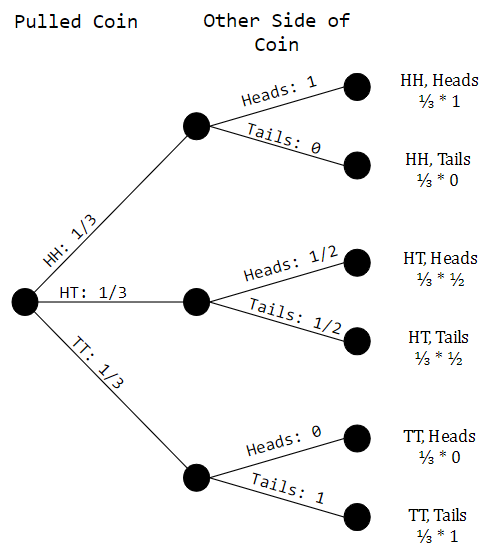
\includegraphics[scale=0.73]{assets/coin.png}
        \end{center}
        So, we want to find the probability that, given we got heads initially, the otherwise will also have heads. This gives us 
        \[\PR[\text{heads} | \text{got heads}] = \frac{\PR[\text{heads given heads}]}{\PR[\text{got heads}]} = \frac{1/3 \cdot 1}{1/2} = \frac{2}{3}.\]
        Note that one way we can think about getting heads is by thinking about the possible face we \emph{can} get; in this case, we can either get $\{H, H, H, T, T, T\}$. We have a $\frac{3}{6} = \frac{1}{2}$ chance of getting heads. 
    \end{mdframed}
\end{mdframed}

\begin{mdframed}
    (Exercise.) Suppose 80\% of people like peanut butter, 89\% like jelly, and 78\% like both. Given that a randomly sampled person likes peanut butter, what's the probability that they also like jelly?

    \begin{mdframed}
        Let $J$ be the event that someone likes jelly and $B$ be the event that someone likes peanut butter. We know that 
        \[PR[B] = 0.80.\]
        We also know that $\PR[J \cap B] = 0.78$ since 78\% of people like \emph{both} peanut butter and jelly. So, 
        \[\PR[J|B] = \frac{\PR[J \cap B]}{\PR[B]} = \frac{0.78}{0.80} = 0.975.\]
    \end{mdframed}
\end{mdframed}

\begin{mdframed}
    Lupus is a medical phenomenon where antibodies that are supposed to attack foreign cells to prevent infections instead see plasma proteins as foreign bodies, leading to a high risk of blood clotting. It is believed that 2\% of the population suffers from this disease. A test for lupus is 98\% accurate if a person actually has the disease, and 74\% accurate if a person does not have the disease. There is a line from the Fox television show House that is often used after a patient tests positive for lupus: ``It's never lupus.'' Do you think there is truth to this statement? Use appropriate probabilities to support your answer.

    \begin{mdframed}
        Consider the following tree diagram: 
        \begin{center}
            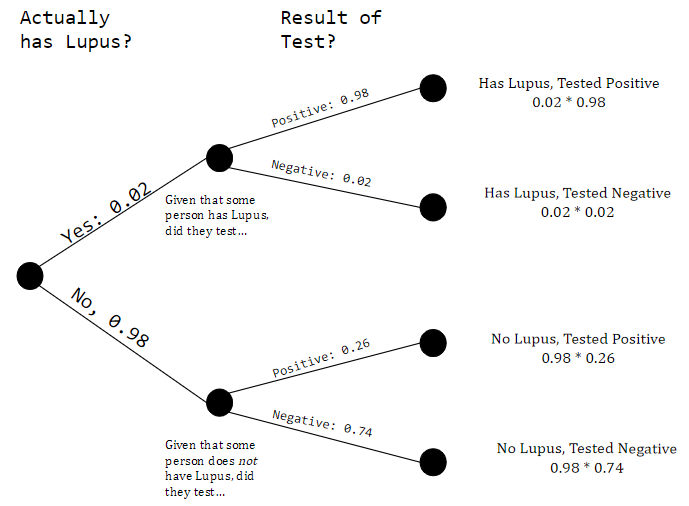
\includegraphics[scale=0.73]{assets/lupus.png}
        \end{center}
        Then, 
        \[\PR[\text{has lupus} | \text{tested positive}] =\frac{\PR[\text{has lupus + tested positive}]}{\PR[\text{tested positive}]} = \frac{0.02 \cdot 0.98}{0.02 \cdot 0.98 + 0.98 \cdot 0.26} \approx 0.07142.\]
        So, there is some truth to the statement since if someone tests positive for lupus, there's only 7.14\% that they have lupus. 
    \end{mdframed}
\end{mdframed}

\begin{definition}{Independent Events}{10:1}
    Fix a probability space. We say that two events $A$ and $B$ are independent if 
    \[\PR[A \cap B] = \PR[A]\PR[B].\]
\end{definition}
Often, it's convenient to reformulate this definition slightly. In the case that $\PR[B] > 0$, \[\PR[A \cap B] = \PR[A] \PR[B] \iff \frac{\PR[A \cap B]}{\PR[B]} = \PR[A].\] However, notice that \[\frac{\PR[A \cap B]}{\PR[B]} = \PR[A | B]\] so it follows that the independence of $A$ and $B$ is equivalent to asserting that \[\PR[A | B] = \PR[A].\] We could interpret this statement as follows: if $A$ and $B$ are independent, then our confidence in $A$ happening does not change at all even if we're told that $B$ happened (or did not happen). More loosely, knowing whether or not $B$ happens tells us ``nothing'' about whether or not $A$ happenes.

\begin{mdframed}
    (Exercise.) The American Community Survey is an ongoing survey that provides data every year to give communities the current information they need to plan investments and services. The 2010 American Community Survey estimates that 14.6\% of Americans live below the poverty line, 20.7\% speak a language other than English at home, and 4.2\% fall into both categories. Is the event that a randomly chosen American lives below the poverty line independent of the event that the person speaks a language other than English at home?

    \begin{mdframed}
        Define 
        \[\PR[\text{Below Poverty Line}] = 0.146,\]
        \[\PR[\text{Speak Language Other Than English}] = 0.207,\]
        \[\PR[\text{Below Poverty Line AND Speak Language Other Than English}] = 0.042.\]
        Using the formula in (\ref{def:10:1}), notice how \[0.042 \neq 0.146(0.207) = 0.030222.\]
    \end{mdframed}
\end{mdframed}

\begin{mdframed}
    (Exercise.) A bag contains 5 red marbles and 3 blue marbles. Two marbles are drawn randomly from the bag: Alejandra takes the first one and Beatrice takes the second. Is the event that Alejandra's marble is blue independent of the event that Beatrice's marble is blue?

    \begin{mdframed}
        No. If Alejandra takes the first marble and doesn't put it back, then it's possible that she took the blue marble, which affects the probability that Beatrice gets a blue marble.
    \end{mdframed}
\end{mdframed}

\begin{definition}{}{}
    Fix a probability space. Two random variables $X$ and $Y$ are \textbf{independent} if the events $X = a$ and $Y = b$ are independent for all pairs $(a, b)$ where $a$ is a value of $X$ and $b$ a value of $Y$.
\end{definition}

\subsection{Index of Coincidence}
Imagine starting with some text consisting of only uppercase alphabet characters. Separate all of the letters from each other. Throw them all into in a bag to shuffle them up. Then draw two letters from it without replacement. What is the probability that the two letters you drew are the same?

\bigskip

We can let $N$ be the total number of letters in the bag. For each letter $\alpha$, let $N_\alpha$ be the number of times that $\alpha$ appears in the bag. Then, $\frac{N_\alpha}{N}$ is the probability that $\alpha$ is the first letter you draw from the bag. After you get that letter, there are $N - 1$ letters left in the bag and $\alpha$ occurs only $N_\alpha - 1$ times, so the probability of drawing $\alpha$ again is $\frac{N_\alpha - 1}{N - 1}$. The overall probability, then, of drawing $\alpha$ twice is \[\frac{N_\alpha (N_\alpha - 1)}{N(N - 1)}.\]

Now, notice that this probability is for \emph{some} letter $\alpha$. However, the question we asked in the first paragraph asks what the probability is of drawing two of the same letters in a row. So, we need to consider every possible letter; therefore, the probability we're looking for is \[\sum_{\alpha \in \{A, \hdots, Z\}} \frac{N_\alpha (N_\alpha - 1)}{N(N - 1)}.\] 

\begin{mdframed}
    (Exercise.) Above we stated that the probability of drawing $\alpha$ for our first letter is $N_\alpha / N$ and the probability of drawing $\alpha$ for our second letter is $(N_\alpha - 1) / (N - 1)$, so the probability of drawing two $\alpha$'s in a row is the product of these. Justify this ``multiplication'' of probabilities using conditional probabilities.

    \begin{mdframed}
        Let $A_{\alpha}$ be the event that the first letter is $\alpha$, and let $B_\alpha$ be the event that the second letter is $\alpha$. Notice how $\PR[A_{\alpha}] = \frac{N_\alpha}{N}$ and $\PR[B_\alpha | A_\alpha] = \frac{N_\alpha - 1}{N - 1}$, so it follows that \[\PR[B_\alpha | A_\alpha] = \frac{\PR[B_\alpha \cap A_\alpha]}{\PR[A_\alpha]} \implies \PR[B_\alpha | A_\alpha] \PR[A_\alpha] = \PR[B_\alpha \cap A_\alpha] \implies \PR[B_\alpha \cap A_\alpha] = \frac{N_\alpha}{N} \frac{N_\alpha - 1}{N - 1}.\]
    \end{mdframed}
\end{mdframed}
Since there are 26 letters in the English alphabet, it turns out to be convenient to normalize this probability we computed above by multiplying by 26. The resulting number gets a special name: 
\begin{definition}{Index of Coincidence}{}
    Let $N$ be the length of some text and, for each letter $\alpha$, let $N_\alpha$ be the number of times $\alpha$ occurs in this text. The \textbf{index of coincidence} of the text, denoted $IC$, is the number \[IC = 26 \sum_{\alpha \in \{A, \hdots, Z\}} \frac{N_\alpha (N_\alpha - 1)}{N(N - 1)}.\]
\end{definition}

\begin{mdframed}
    Suppose that you start with a text where every letter appears equally often. What would the index of coincidence of such a text be?

    \begin{mdframed}
        If every letter appears equally often, then we know that there will be $\frac{1}{26}N$ of each letter. Then, the index of coincidence is given by 
        \begin{equation*}
            \begin{aligned}
                IC &= 26 \sum_{\alpha \in \{A, \dots, Z\}} \frac{\frac{1}{26}N (\frac{1}{26}N - 1)}{N(N - 1)} \\ 
                    &= 26 \frac{\frac{1}{26}N (\frac{1}{26}N - 1)}{N(N - 1)}  \sum_{\alpha \in \{A, \dots, Z\}} 1 \\ 
                    &= 26 \frac{\frac{1}{26}N (\frac{1}{26}N - 1)}{N(N - 1)} 26 \\ 
                    &= \frac{N (\frac{1}{26}N - 1)}{N(N - 1)} 26 \\ 
                    &=  \frac{(\frac{1}{26}N - 1)}{(N - 1)} 26 \\ 
                    &= \frac{N - 26}{N - 1} 
            \end{aligned}
        \end{equation*}
        Notice how, as $N \mapsto \infty$, $\frac{N - 26}{N - 1} \approx 1$, so it follows that the index of coincidence would be approximately 1.0.
    \end{mdframed}
\end{mdframed}


\begin{mdframed}
    (Exercise.) What is the largest possible index of coincidence? What kind of text would result in an index of coincidence that's as large as possible?

    \begin{mdframed}
        Suppose only one letter was in some given text. Then, $N_\alpha = \begin{cases}
            N & \text{if } \alpha \text{ is that letter} \\ 
            0 & \text{otherwise}
        \end{cases}$ and 
        \begin{equation*}
            \begin{aligned}
                IC &= 26 \sum_{\alpha \in \{A, \hdots, Z\}} \frac{N_\alpha (N_\alpha - 1)}{N(N - 1)} \\
                    &= 26 (\hdots + 0 + \frac{N(N - 1)}{N(N - 1)} + 0 + \hdots) \\ 
                    &= 26 (\hdots + 0 + 1 + 0 + \hdots) \\ 
                    &= 26 (1) \\ 
                    &= 26.
            \end{aligned}
        \end{equation*}
        So, the largest possible index of coincidence is 26 and the resulting text would only have one letter.
    \end{mdframed}
\end{mdframed}

\begin{mdframed}
    (Exercise.) Let $N$ be the length of some text and, for each letter $\alpha$, let $N_\alpha$ be the number of times $\alpha$ occurs in this text. Let $p_\alpha = N_\alpha / N$. Show that, if $N$ is very large, then 
    \[IC \approx 26 \sum_{\alpha \in \{A, \hdots, Z\}} p_\alpha^2.\]

    \begin{mdframed}
        Note that 
        \begin{equation*}
            \begin{aligned}
                IC &= 26 \sum_{\alpha \in \{A, \hdots, Z\}} \frac{N_\alpha (N_\alpha - 1)}{N(N - 1)} \\
                    &\approx 26 \sum_{\alpha \in \{A, \hdots, Z\}} p_{\alpha} p_{\alpha} && \text{Assume } N \text{ is very large} \\ 
                    &= 26 \sum_{\alpha \in \{A, \hdots, Z\}} p_\alpha^2.
            \end{aligned}
        \end{equation*}
    \end{mdframed}
\end{mdframed}

As we've seen, relative frequencies of letters in English are roughly stable from text to text, at least for sufficiently long texts. Correspondingly, the index of coincidence is also roughly stable from text to text! Here is the relevant heuristic:

\begin{mdframed}
    (Heuristic.) The index of coincidence of long English plaintext is 
    \begin{itemize}
        \item typically around 1.75, and 
        \item almost always between 1.5 and 2. 
    \end{itemize}
\end{mdframed}

Note that, based on the exercise above,
\[IC \approx 26 \sum_{\alpha \in \{A, \hdots, Z\}} p_\alpha^2.\]
The right-hand side always exactly the same if we perform a simple substitution on our text. 
\begin{mdframed}
    (Example.) For example, suppose the letter \code{E} has a relative frequency of 13\% in some plaintext. Then, $p_E^2 \approx 0.13^2$ will appear as a summand in the above expression for the IC of this plaintext. 

    \bigskip 

    Now, suppose we perform a simple substitution that converts \code{E} to \code{Q}. Then, $p_Q^2 \approx 0.13^2$ will appear as a summand of the IC for the ciphertext.
\end{mdframed} 
The subscript is different, but the value is exactly the same. So, since we're summing over all the letters, the value of IC does not change when we performa  simple substitution.

\begin{mdframed}
    (Exercise.) Suppose some English plaintext is encrypted using a transposition cipher (e.g., rectangular transposition). How will the index of coincidence of the plaintext compare to that of the ciphertext?

    \begin{mdframed}
        Because rectangular transposition (and any cipher that just rearranges text around) simply rearranges the letters of the plaintext around, the index of coincidence for the plaintext will be exactly the same as the index of coincidence for the ciphertext.

        \bigskip 

        In particular, this means that the index of coincidence of the ciphertext will probably have the same properties as the described heuristic above.
    \end{mdframed}
\end{mdframed}


\subsection{Breaking the Vigenere Cipher}
With the index of coincidence in hand, we can now break the Vigenere cipher. Although this isn't the \href{https://en.wikipedia.org/wiki/Kasiski_examination}{first method} that was used to break said cipher, it does use the index of coincidence.

\bigskip 

Suppose we start with ciphertext which is known for being encrypted using the Vigenere cipher:
\begin{mdframed}
    \begin{verbatim}
        IKGWERTZONXEULTEZWHWXTYHSZKEGQOJNENRUDJGFRNKUISLDZOMKDKWZHVU
        OSJLFZEJJONQHWVRFEATRYIDIKKDKKEHNAEWOEYFIRMLNIENIFMAJKELXAMH
        RKKDKKEEUOIVADUNVRNLNEERNKKNJHHWNAUKESXDYLSHGRVQTKGNUFOEVAEL
        OFYRVSESZYVWSLOLCLDGTTCLKWHEZQGGATZQTZKDRUKFUWRQDAJOEWLAQESH
        IFMLVITTEMPVEDLIEWHAYGILMZUUJHIUGNERTZKLGLTAYHROLTKGCDDONEEW
        HWEL...\end{verbatim}
\end{mdframed}
Then, we can try to decrypt the ciphertext like so: 
\begin{enumerate}
    \item First, make a guess for the ``period'' (i.e., the length of the keyword). Suppose we guess a period of 5. Then, we can break the ciphertext into rows of that length. 
    \begin{verbatim}
        IKGWE 
        RTZON 
        XEULT 
        EZWHW 
        XTYHS 
        ZKEG…\end{verbatim}

    If the period we've guessed is correct, \textbf{each column of this rectangle was encryped using a Caesar cipher with the same shift}. This means that we should be able to detect that our guess for the period is correct by examining indices of coincidence. If every column has an index of coincidence in the range that's expected of English text, our guess for the period is probably correct. Otherwise, we should try a different period. 

    \bigskip 

    In our example above, if we guess a period of 5, it turns out that the indices of coincidence of the five columns are 1.13, 1.11, 1.18, 1.15, and 1.15, respectively. That's outside the range that's expected of English text, so our guess of 5 is probably is wrong. If we try a period of 6, we find that the indices of coincidence are 1.75, 1.77, 1.73, 1.72, 1.79, and 1.74, respectively -- all in the right range. So, the period of 6 is probably correct. 

    \item Once we find a probable guess for the period, we're in the clear. Then, we just have to figure out what the shift is for each column, which we can do using basic frequency analysis. Recall that the most frequent letter in each column should correspond to \code{E}, so we should guess that the shift for that column is the shift that moves \code{E} to the most frequent letter (If that doesn't work we might try shifting so that the second most frequent letter in that column moves to \code{E} instead.)
\end{enumerate}



\subsection{Known-Plaintext Attack on Simple Substitution}
So far, we've studied a few techniques for conducting ciphertext-only attacks on various ciphers, i.e., ciphers where the only information Eve knows to begin with is which cipher was used to encrypt a message and has no information about the message itself. 

\bigskip 

Now, let's suppose Eve \emph{does} have some partial information about the plaintext itself. Specifically, we'll consider the situation where Eve already knows that a certain word appears at least once in the plaintext. As it turns out, we can use the $G$-test statistic to help us make good guesses here. 

\bigskip 

Suppose, for example, Eve intercepts some ciphertext, known to be encrypted using a \textbf{simple substitution}:
\begin{verbatim}
    CUXQAUDRERAUFJUCKRACUXQAUDRXFGAUFJUCKRACUXQAUDRQWRFJXCAOFKCUXQAUDRQWR
    FJJFFSCADZRAACUXQAUDRRNFYDFJERSCRJCUXQAUDRRNFYDFJCZYGROMSCUPCUXQAUDRA
    RQAFZFJSCWDUCUXQAUDRARQAFZFJOQGTZRAACUXQAUDRANGCZWFJDFNRCUXQAUDRXCZUR
    GFJORANQCGXRDQORLRGPUDCZWERJFGRMAXRDQOZFUDCZWERJFGRMAXRXRGRQSSWFCZWOC
    GRYUUFDRQLRZXRXRGRQSSWFCZWOCGRYUUDRFUDRGXQPCZADFGUUDRNRGCFOXQAAFJQGSC
    TRUDRNGRARZUNRGCFOUDQUAFKRFJCUAZFCACRAUQMUDFGCUCRACZACAUROFZCUAERCZWG
    RYRCLROJFGWFFOFGJFGRLCSCZUDRAMNRGSQUCLRORWGRRFJYFKNQGCAFZFZSPUDRGRXRG
    RQTCZWXCUDQSQGWRHQXQZOQIMRRZXCUDQNSQCZJQYRFZUDRUDGFZRFJRZWSQZOUDRGRXR
    GRQTCZWXCUDQSQGWRHQXQZOQIMRRZXCUDQJQCGJQYRFZUDRUDGFZRFJJGQZYRCZEFUDYF
    MZUGCRACUXQAYSRQGRGUDQZYGPAUQSUFUDRSFGOAFJUDRAUQURNGRARGLRAFJSFQLRAQZ
    OJCADRAUDQUUDCZWACZWRZRGQSXRGRARUUSROJFGRLRGCUXQAUDRPRQGFJFMGSFGOFZ...\end{verbatim}
Now, more importantly, suppose Eve already knows that the word \code{LONDON} occurs at least \emph{once} in the plaintext. How does the codebreaking process change? 

\begin{enumerate}
    \item Notice how, in the word \code{LONDON}, the first 4 letters are all distinct, the 5th letter is the same as the 2nd letter, and the 6th letter is the same as the 3rd letter. This pattern will be \textbf{preserved} by simple substitution, so somewhere in the ciphertext, we should find that same sequence. If we can find such a sequence, it suggests that the letters \code{L}, \code{O}, \code{N}, \code{D} should be matched.  
    
    \bigskip

    There are 18 sequences in this ciphertext\footnote{Not all patterns may show up above in the ciphertext; most of the ciphertext has been omitted for brevity.} that fits this pattern
    \begin{verbatim}
        SCUPCU      GKROKR
        RACZAC      MUFJUF
        OFGJFG      SXQAXQ
        ZUDRUD      SFZOFZ
        ZUDRUD      UQZOQZ
        SFZOFZ      SFZOFZ
        ARZURZ      RZUCZU
        UDCZDC      GCZWCZ
        RAFJAF      QZWCZW\end{verbatim}

    If we were just brute-forcing through all possible substitutions, the number of possibilities for matching the letters \code{L}, \code{O}, \code{N}, and \code{D} would be 
    \[26 \cdot 26 \cdot 24 \cdot 23 = 358800,\]
    which is already significantly less than if we didn't know about the pattern beforehand. 

    \item The key observation is that the relative frequencies of the letters \code{L}, \code{O}, \code{N}, and \code{D} in some sample of plaintext English should match the relative frequencies of the corresponding ciphertext letters. We can measure the deviations between frequencies using $G$, so we can compute $G$ for each of the 15 possible matchings and use that to help guide our choices. How do we calculate $G$? Let's take a look at one of these calculations in detail. 
    
    \begin{itemize}
        \item Start by looking at some sample English text (e.g., the Declaration of Independence) and throwing out all the letters \emph{except} \code{L}, \code{O}, \code{N}, and \code{D}. If we do so, we find the following distributions:
        \begin{center}
            \begin{tabular}{|c|c|c|c|c|c|}
                \hline 
                    & \code{L} & \code{O} & \code{N} & \code{D} & Total \\
                \hline 
                Count in Sample & 228 & 513 & 483 & 252 & 1476 \\ 
                Percent in Sample & 15.4\% & 34.8\% & 32.7\% & 17.1\% & 100\% \\ 
                \hline 
            \end{tabular}
        \end{center}
        Let's suppose we think the first sequence (out of all possible sequences above), \code{SCUPCU}, corresponds to \code{LONDON}. This would mean that \code{S} is matched to \code{L}, \code{C} to \code{O}, \code{U} to \code{N}, and \code{P} to \code{D}. We can then go through our ciphertext and count the instances of \code{S}, \code{C}, \code{U}, and \code{P} (throwing out all other letters as usual) and then fill in the first row of the table below: 
        \begin{center}
            \begin{tabular}{|c|c|c|c|c|c|}
                \hline 
                    & \code{S} & \code{C} & \code{U} & \code{P} & Total \\
                \hline 
                Observed in Ciphertext & 146 & 293 & 429 & 83 & 951 \\ 
                Expected in Ciphertext & 146.9 & 330.5 & 311.2 & 162.4 & 951 \\ 
                \hline 
            \end{tabular}
        \end{center}
    \end{itemize}
    Here, the expected values were obtained by taking the percent in sample from the first table and then multiplying those percentages by the observed values in the ciphertext. To see why this is the case, note that 
    \begin{itemize}
        \item We saw that $15.4\%$ of the letters \code{L}, \code{O}, \code{N}, \code{D} should be \code{L}. 
        \item If \code{L} corresponds to \code{S} in the ciphertext, then we would expect \[0.154 \cdot 951 \approx 146.9\] letters of the ciphertext to be \code{S}. 
    \end{itemize}
    In any case, we can now compute the $G$-value; 
    \begin{equation*}
        \begin{aligned}
            G &= 2 \sum O\ln\left(\frac{O}{E}\right) \\ 
                &\approx 2\left(146 \ln\left(\frac{146}{146.9}\right) + 293 \ln\left(\frac{293}{330.5}\right) + 429 \ln\left(\frac{429}{311.2}\right) + 83 \ln\left(\frac{83}{162.4}\right) \right) \\ 
                &\approx 91.6.
        \end{aligned}
    \end{equation*}

    \begin{mdframed}
        (Exercise.) The values of $G$ are approximated by a chi-square distribution with $k$ degrees of freedom. What is $k$? What is the value of the integral \[\int_{91.6}^{\infty} f_{k}(x) dx,\] i.e., the $p$-value? Based on this, does it seem likely that \code{SCUPCU} is a correct match for London? 
        \begin{mdframed}
            We have four possible observations to make; either one for \code{S}, \code{C}, \code{U}, or \code{P}. Let $n = 4$ so that $k = n - 1 = 4 - 1 = 3$.
            % TODO $p$-value.
        \end{mdframed}
    \end{mdframed}

    We can then do analogous calculations of $G$ for the other 14 possibilities. The results are as follows: 
    \begin{center}
        \begin{tabular}{|c|c|}
            \hline 
            Ciphertext Match & $G$ \\ 
            \hline 
            SCUPCU & 91.6 \\ 
            RACZAC & 602.9 \\ 
            OFGJFG & 34.5 \\ 
            ZUDRUD & 442.5 \\ 
            SFZOFZ & 7.8 \\ 
            ARZURZ & 160.5 \\ 
            UDCZDC & 354.4 \\ 
            RAFJAF & 597.0 \\ 
            GKROKR & 490.8 \\ 
            MUFJUF & 39.3 \\ 
            SXQAXQ & 284.8 \\
            UQZOQZ & 223.0 \\
            RZUCZU & 444.8 \\ 
            GCZWCZ & 162.4 \\ 
            QZWCZW & 533.3 \\ 
            \hline 
        \end{tabular}
    \end{center}
    Recall that smaller values of $G$ mean that the distributions are closer together, so the most likely match for \code{LONDON} appears to be \code{SFZOFZ}. Of course, it's possible that \code{SFZOFZ} is not the correct match, but if we make that guess and then it seems like the decryption is turning out to be nonsense, we can just go back and try the one option with the next lowest value of $G$. 

    \bigskip 

    As we've seen, it's usually easy to guess which letters correspond to \code{E} and \code{T}. So, we now have a systematic way of identifying the letters \code{L}, \code{O}, \code{N}, and \code{D} as well. 
\end{enumerate}


\subsection{Perfect Secrecy}
Let's now discuss cryptosystems in some generality. The point of this section is to show what it means when we say that the one-time pad achieves perfect secrecy.

\bigskip 

Let's introduce the general framework. 
\begin{itemize}
    \item From Eve's perspective, it makes sense to consider Alice's choice of a plaintext message as a \emph{random variable} $M$ whose set of values $\mathscr{M}$ represents all possible plaintext messages. By saying that $M$ is a random variable, we're introducing probabilities associated to every possible plaintext message, and we're assuming that Eve knows this probability distribution. 
    \begin{itemize}
        \item For example, $\mathscr{M}$ might be the set of all strings in the letters \code{A}-\code{Z}, and we might deem the plaintext \code{QUIZ} to be less probable than the plaintext \code{THEN} on the basis that the former uses much more infrequent letters than the latter. 
        \item Alternatively, we could assign probabilities based on bigram frequencies instead of single-letter frequencies. 
    \end{itemize}
    It doesn't matter \emph{how} we assign probabilities; the point is just that any plaintext message has a probability assigned to it. 

    \item We can model known-plaintext attacks in at least two ways. Suppose, for example, Eve knows that the plaintext must contain the word \code{LONDON}. 
    \begin{enumerate}
        \item The first way to model a known-plaintext attack is to assign a probability of 0 to every plaintext message that \emph{doesn't} contain the \code{LONDON} as a substring. 
        \item The second way is to simply eliminate all strings that do not contain \code{LONDON} from our set of values $\mathscr{M}$. 
    \end{enumerate}
    It's more convenient to use the latter method of modeling known-plaintext attacks, since it allows us to assume that \[\PR[M = m] \neq 0\] for all $m \in \mathscr{M}$, and so we'll assume this from here on out.  
\end{itemize}
All of this brings us to the following definition of a cryptosystem. 
\begin{definition}{Cryptosystem}{}
    A \textbf{cryptosystem} (on $M$) consists of the following data: 
    \begin{itemize}
        \item A random variable $K$ whose set of values $\mathscr{K}$ represents the set of all possible keys. 
        \item A set $\mathscr{C}$ of all possible ciphertext. 
        \item An encryption function \[E: \mathscr{K} \times \mathscr{M} \mapsto \mathscr{C},\] which means that $E$ takes as input a key $k \in \mathscr{K}$ and a plaintext message $m \in \mathscr{M}$ and outputs a corresponding ciphertext $E(k, m) \in \mathscr{C}$. 
        \item A decryption function \[D: \mathscr{K} \times \mathscr{C} \mapsto \mathscr{M},\] which means that $D$ takes as input a key $k \in \mathscr{K}$ and a ciphertext $c \in \mathscr{C}$ and outputs a corresponding plaintext message $D(k, c) \in \mathscr{M}$. 
    \end{itemize}
    In particular, we require that 
    \[D(k, E(k, m)) = m\]
    for any key $k \in \mathscr{K}$ and any plaintext message $m \in \mathscr{M}$, i.e., that a plaintext can be recovered from its encryption. Once we've specified the above data, we also define the random variable $C = E(K, M)$ to model an observation of the ciphertext. 
\end{definition}

\begin{mdframed}
    (Example.) Consider the Caesar cipher. The sets $\mathscr{M}$ and $\mathscr{C}$ are both equal to the set of all possible strings in the capital letters \code{A} through \code{Z}, and the key string $\mathscr{K}$ is the set of all possible shifts, i.e. \[\mathscr{K} = \{0, 1, 2, \hdots, 24, 25\}.\] Given $k \in \mathscr{K}$ and $m \in \mathscr{M}$, the string $E(k, m)$ is the result of applying the Caesar cipher with shift $k$ to $m$, i.e., by adding $k$ mod 26 to the numbers 0-25 corresponding to each letter \code{A}-\code{Z} in $m$. To fully specify the cryptosystem, we should also assign probabilities to each of the keys; for example, we might assume that $\mathscr{K}$ is uniform. 

    \bigskip 

    This is not necessarily the only way to fit the Caesar cipher into the above framework. For example, if you like, you can fix an upper bound on the length of the strings involved so that $\mathscr{M}$ and $\mathscr{C}$ are finite. You could also decide that the key space is just $\{1, 2, \hdots, 25\}$, if you don't want to consider a shift of 0 to be a valid key. You could also choose a non-uniform distribution for the random variable $K$.  
\end{mdframed}

\begin{definition}{Perfect Secrecy}{}
    A cryptosystem achieves \textbf{perfect secrecy} if $M$ and $C$ are independent random variables. 
\end{definition}
In other words, for any plaintext message $m$ and any encrypted message $c$, we should have 
\[\PR[M = m | C = c] = \PR[M = m].\]
Heuristically, this means that observing $C = c$ provides Eve with no additional information whatsoever about $M$; the best guesses that she might have made about the plaintext message before she intercepted the ciphertext do not change even after she intercepts the ciphertext. 

\bigskip 

Recall that the attacks on cryptosystems that we've seen so far exploit the fact that those cryptosystems fail to achieve perfect secrecy. When we conduct frequency analysis on simple substitution, for example, we are using the fact that certain plaintexts become more likely after observing  a given ciphertext, e.g., the plaintexts in which the letter \code{E} appears in the same positions in which the most frequenct letter of the ciphertext appears. 

\bigskip 

How do we achieve perfect secrecy? The first observation to make here is that achieving perfect secrecy requires having a lot of keys. More precisely, 

\begin{lemma}{}{}
    Suppose a cryptosystem achieves perfect secrecy. Then, the number of keys must be at least as large as the number of ``possible'' ciphertexts (i.e., ciphertexts $c \in \mathscr{C}$ such that $\PR[C = c] \neq 0$).
\end{lemma}

Having observed this, here is a result that gives us a way to achieve perfect secrecy.

\begin{theorem}{Perfect Secrecy}{}
    A cryptosystem achieves perfect secrecy if it satisfies all of the following conditions: 
    \begin{itemize}
        \item $K$ is uniform. 
        \item $K$ and $M$ are independent.
        \item For every plaintext message $m \in \mathscr{M}$ and every ciphertext $c \in \mathscr{C}$, there exists a unique $k \in \mathscr{K}$ such that $E(k, m) = c$. 
    \end{itemize}
\end{theorem}
We now want to show that the ``one-time pad achieves perfect secrecy.'' Remember that the one-time pad is a special case of the Vigenere cipher. Fix a period $p$ and 
\begin{itemize}
    \item let $\mathscr{K}$ be the set of all sequences $\{a_1, \hdots, a_p\}$, where $a_1, \hdots, a_p \in [0, 1, 2, \hdots, 24, 25]$. Fix a message length $r$, and 
    \item let $\mathscr{M}$ and $\mathscr{C}$ be the set of all strings in the letters \code{A}-\code{Z} of length $r$. 
    \item Also note that if Eve intercepts a ciphertext of length $r$ that she knows to be encrypted using a Vigenere cipher, she also knows the plaintext must have length $r$, so she can assign probability 0 to all messages of other lengths. In other words, it's reasonable to eliminate all messages of other lengths from our message spaces. 
\end{itemize}
We then have the Vigenere encryption and decryption functions $E: \mathscr{K} \times \mathscr{M} \mapsto \mathscr{C}$ and $D: \mathscr{K} \times \mathscr{C} \mapsto \mathscr{M}$.  Applying Vigenere encryption to a message of length $r$ will always just use the first $\min\{r, p\}$ of the $p$ numbers in our key sequence, so might as well replace $p$ with $\min\{r, p\}$ in order to assume that $p \leq r$. 

\begin{lemma}{}{}
    Using the notation we've just introduced, we have $p = r$ if and only if, for every plaintext message $m \in \mathscr{M}$ and every ciphertext, there exists a unique $k \in \mathscr{K}$ such that $E(k, m) = c$. 
\end{lemma}
With this in mind, recal lsome of the assumptions we made when we were discussing the one-time pad when we first introduced it. 
\begin{itemize}
    \item The key sequence needs to be ``totally random.'' We can now formalize this by saying that we want our random variable $K$ to be uniform. 
    \item The key sequence must be ``unrelated to the plaintext.'' We can now formalize this by saying that $K$ and $M$ be independent random variables. 
    \item The key sequence must be as long as the plaintext. In the notation we just introduced, this is the requirement that $p \geq r$, but we already assumed that $p \leq r$ so in fact this is equivalent to saying $p = r$ and, in the lemma above, we saw that this is equivalent to saying that, for any $m \in \mathscr{M}$ and $c \in \mathscr{C}$, there exists a unique $k \in \mathscr{K}$ such that $E(k, m) = c$. 
\end{itemize}
In other words, these three assumptions we made coincide exactly with the conditions that appear in the Perfect Secrecy Theorem! We have now proved what we want to prove:
\begin{corollary}{}{}
    The one-time paid achieves perfect secrecy.
\end{corollary}













\newpage 
\section{Modern Cryptography}
Modern cryptography generally begins with two, related, desires 
\begin{itemize}
    \item In all the ciphers we've seen so far, we assume Alice and Bob have some way of sharing a key. We haven't said much about \emph{how} that happens, and we've also seen that the perfect secrecy requires very long keys. How can Alice and Bob share a long key with each other without Eve finding out about it? 
    \item None of the ciphers we've seen so far is robust against chosen-plaintext attacks. If Eve has the ability to request the ciphertexts for any plaintexts she likes, she can gradually get more information about the key until she can break the code. Recall that the one-time pad is only safe if the key is only used once. 
\end{itemize}
We would like a cryptosystem where the \emph{decryption key} is only known to Bob. Alice and Eve and everyone else in the world has access to Bob's encryption key and can encrypt messages for Bob to see, but then only Bob can recover the plaintext. This allows us to avoid Alice and Bob having to share a common key, and would allow Eve to generate ciphertexts for any plaintext of her choosing while also making sure that the cryptosystem is safe against chosen-ciphertext attacks. 

\bigskip 

It turns out that there are a number of cryptosystems of this type, and they all fall under the heading of \textbf{public-key cryptography}, because the encryption key can be made public to the world. A recurring theme behind public-key cryptosystems is a ``one-way function,'' which is a function that's easy to compute but hard to invert. 

\subsection{Interlude: Primes} 
\begin{definition}{Prime}{}
    A positive integer $p \geq 2$ is \textbf{prime} if its only positive divisors are 1 and itself. An integer $n \geq 2$ that is not prime is called \textbf{composite}.
\end{definition}
For example, 5 is prime because 1 and 5 are its only divisors. 4, on the other hand, is not prime, since 2 is a divisor of 4 (in addition to 1 and 4). 

\begin{mdframed}
    (Exercise.) The ``twin prime conjecture'' is a famous open problem which says that there are infinitely many “twin primes,” ie, pairs of primes that are 2 apart. For example, 3 and 5 are twin primes, as are 5 and 7, or 11 and 13. Give five more examples of twin primes.
    
    \begin{mdframed}
        The following pairs are five other examples:
        \[(17, 19), (29, 31), (41, 43), (59, 61), (71, 73).\]
    \end{mdframed}
\end{mdframed}

\begin{mdframed}
    (Exercise.) There is a version of the twin prime conjecture which says that every even integer can be written as the difference of consecutive primes in infinitely many ways. For example, we have: \[6 = 29 - 23 = 137 - 131 = 599 - 593 = \hdots.\]
    Express the integer 10 as the difference of two consecutive primes in five different ways.
    \begin{mdframed}
        Five other ways include: 
        \[10 = 13 - 3 = 17 - 7 = 29 - 19 = 41 - 31 = 71 - 61.\]
    \end{mdframed}
\end{mdframed}

\begin{mdframed}
    (Exercise.) Explain why, if an integer $n \geq 2$ is composite, it must be divisible by a prime $p$ such that $p \leq \sqrt{n}$. Use this fact to determine whether or not 701 is prime. 

    \begin{mdframed}
        \begin{proof}
            Suppose $n$ is composite. Then, we can write \[n = ab\] such that $a, b$ are integers and $1 < a < n$, $1 < b < n$, and WLOG $a \leq b$.
            
            \bigskip 
            
            Further suppose that $a > \sqrt{n}$. Then, $b \geq a > \sqrt{n}$. However, if $b \geq a > \sqrt{n}$, then \[ab > \sqrt{n}\sqrt{n} = n,\] a contradiction (since we wrote that $n = ab$). Therefore, $a \leq \sqrt{n}.$ We know that there exists some prime $p$ which divides $a$, so it follows that $p \leq a$ and $p \leq \sqrt{n}$.  
        \end{proof}
    \end{mdframed}
\end{mdframed}

\subsubsection{Ubiquity of Primes}
Every positive integer $n \geq 2$ can be written as a product of primes. For example, $18 = 2 \cdot 3^2$ and both 2 and 3 are primes. An expression of an integer $n \geq 2$ as a product of primes is called a \emph{prime factorization} of $n$.

\begin{theorem}{Fundamental Theorem of Arithmetic}{}
    Any positive integer $n \geq 2$ has a unique prime factorization. In other words, there exists an expression \[n = p_1^{e_1} p_2^{e_2} \hdots p_r^{e_r}\] such that $p_1, \hdots, p_r$ are primes and $e_1, \hdots, e_r$ are positive integers, and the expression is unique up to reordering the indices. 
\end{theorem}
For example, $60 = 2^2 \cdot 3^1 \cdot 5^1$ is a unique prime factorization of 60; the only other prime factorization involves reordering the factors around. 

\begin{mdframed}
    (Example.) Find the prime factorizations of 1231 and of 1232.

    \begin{mdframed}
        \begin{itemize}
            \item For 1231, note that 
            \[1231 = 1231 \cdot 1.\]

            \item For 1232, note that 
            \[1232 = 616 \cdot 2 = 308 \cdot 2^2 = 154 \cdot 2^3 = 77 \cdot 2^4 = 11 \cdot 7 \cdot 2^4.\]
        \end{itemize}
    \end{mdframed}
\end{mdframed}


\begin{mdframed}
    (Exercise.) 
    \begin{enumerate}
        \item Find all prime factors of $50!$. (Just a list of the prime factors is sufficient; you don't need to find the exponents of the prime factorization for this part.)
        \begin{mdframed}
            Note that \[50! = 50 \cdot 49 \cdot 48 \cdot \hdots \cdot 3 \cdot 2 \cdot 1.\]
            In particular, any composite number less than or equal to 50 can be decomposed into primes that are also less than or equal to 50. Thus, we have \[2, 3, 5, 7, 11, 13, 17, 19, 23, 29, 31, 37, 41, 43, 47.\] 
        \end{mdframed}
        \item Find the prime factorization of $10!$. 
        \begin{mdframed}
            We know that 
            \[10! = 10 \cdot 9 \cdot 8 \cdot 7 \cdot 6 \cdot 5 \cdot 4 \cdot 3 \cdot 2,\]
            where 
            \[10 = 5 \cdot 2,\]
            \[9 = 3^2,\]
            \[8 = 2^3,\]
            \[7 = 7 \cdot 1,\]
            \[6 = 3 \cdot 2,\]
            \[5 = 5 \cdot 1,\]
            \[4 = 2 \cdot 2,\]
            \[3 = 3 \cdot 1,\]
            \[2 = 2 \cdot 1.\]
            So, 
            \[10! = 2^8 \cdot 3^4 \cdot 5^2 \cdot 7.\]
        \end{mdframed}
        \item Find the prime factorization of $11! / 2^8$. 
        \begin{mdframed}
            We know that
            \begin{equation*}
                \begin{aligned}
                    \frac{11!}{2^8} &= \frac{11 \cdot 10 \cdot 9 \cdot 8 \cdot 7 \cdot 6 \cdot 5 \cdot 4 \cdot 3 \cdot 2}{2^8} \\ 
                        &= \frac{11 \cdot (5 \cdot 2) \cdot (3^2) \cdot (2^3) \cdot 7 \cdot (2 \cdot 3) \cdot 5 \cdot (2^2) \cdot 3 \cdot 2}{2^8} \\ 
                        &= 11 \cdot 5 \cdot (3^2) \cdot 7 \cdot 3 \cdot 5 \cdot 3 \\ 
                        &= (3^2) \cdot 3 \cdot 3 \cdot 5 \cdot 5 \cdot 7 \cdot 11 \\ 
                        &= 3^4 \cdot 5^2 \cdot 7 \cdot 11.
                \end{aligned}
            \end{equation*}
            Alternatively, 
            \begin{equation*}
                \begin{aligned}
                    \frac{11!}{2^8} &= \frac{11 \cdot 10!}{2^8} \\
                        &= \frac{11 \cdot 2^8 \cdot 3^4 \cdot 5^2 \cdot 7}{2^8} \\ 
                        &= 11 \cdot 3^4 \cdot 5^2 \cdot 7.
                \end{aligned}
            \end{equation*}
        \end{mdframed}
    \end{enumerate}
\end{mdframed}

\begin{lemma}{Euclid's Lemma}{}
    Suppose $a$ and $b$ are integers and that $d$ is a divisor of $ab$ such that $\gcd(a, b) = 1$. Then, $d$ is a divisor of $b$. 
\end{lemma}

\begin{proof}
    By Bezout's theorem, there exists $x$ and $y$ such that \[1 = \gcd(a, d) = ax + dy.\] Multiplying this by $b$ gives us \[b = abx + bdy.\] Observe that $d$ divides $bdy$, and it also divides $ab$. Thus, $d$ divides the sum $abx + bdy = b$. 
\end{proof}

\subsubsection{Scarcity of Primes \& Difficulty of Factoring}
Having made the observation that primes are ``ubiquitous,'' we should also note that primes are ``scarce.'' The first sense is a literal sense: as a proportion of all integers, very few integers end up being prime. The second sense is that prime factorizations are difficult to actually calculate, even for moderately large numbers. 

\bigskip 

The naive way to find a prime factorization is to figure out what the factors are.
\begin{mdframed}
    (Example.) Suppose we want to find the prime factorization of 75. First, we note that 2 does not divide 75. We then see that 3 does divide 75, and so we're left with 25 ($75 / 3 = 25$). Now, 3 no longer divides 25, and neither does 4. However, 5 does divide 25, so we're left with 5 ($25 / 5 = 5$). Since 5 divides itself, we're left with 1 ($5 / 5 = 1$), so the prime factorizations are \[75 = 3^1 \cdot 5^2.\]
\end{mdframed}
This process is extremely slow as the number gets larger or, more specifically, as the prime factors of the number get larger. 

\bigskip 

There are a number of deep, sophisticated, and clever techniques to speed this process up\footnote{Which will not be covered in this course.}, but no one has yet found a factorization algorithm for classical computers that is substantially better than the naive method we just described. The difficulty of factoring can be leveraged to build modern cryptosystems that are in widespread use today. 

\bigskip 

Some things to further consider: 
\begin{itemize}
    \item Just because there are no substantially better algorithm for finding the prime factorizations doesn't mean one does exist. In other words, there could be an algorithm for finding prime factorizations in an efficient way, but we haven't found it. 
    \item Efficient factorization algorithms exist for \emph{quantum computers}, but quantum computing hardware has not yet caught up to our theoretical knowledge, so our modern cryptosystems are still safe for now. That being said, this won't last for much longer and so we will soon need new cryptosystems that are secure against quantum computers.
\end{itemize}

\bigskip 

The difficulty of factoring suggests that the function $\mu$, which takes as input two prime numbers $p$ and $q$ and outputs the product \[\mu(p, q) = pq\] is our first example of a \textbf{one-way} function. It's very easy to compute the product of two primes but, if the primes are large, it'll be very hard to invert this function (i.e., find the prime factors of some given number that has two large prime factors). This is the one-way function on which RSA is based, as we will soon see. 


\subsection{Euler's Phi Function}
\begin{definition}{Euler's Phi Function}{}
    For a positive integer $n$, let $\phi(n)$ denote the number of integers $r$ with $0 \leq r < n$ and $\gcd(n, r) = 1$. The function $n \mapsto \phi(n)$ is called \emph{Euler's phi function} (or \emph{Euler's totient function}).
\end{definition}

For example, when we were counting that there are 312 affine encryption functions available in English, part of the process involved counting the number of numbers relatively prime to 26, and we found it was 12. Now, we can say this as \[\phi(26) = 12.\]

\begin{mdframed}
    (Exercise.) Compute $\phi(12)$, $\phi(13)$, $\phi(14)$, and $\phi(15)$. 
    \begin{mdframed}
        \begin{itemize}
            \item For $\phi(12)$, we know that 
            \[\gcd(1, 12) = \gcd(5, 12) = \gcd(7, 12) = \gcd(11, 12) = 4,\]
            so $\phi(12) = 4$. 

            \item Because $13$ is prime, $\phi(13) = 12$. 
            
            \item For $\phi(14)$, we know that 
            \[\gcd(1, 14) = \gcd(3, 14) = \gcd(5, 14) = \gcd(9, 14) = \gcd(11, 14) = \gcd(13, 14) = 1,\]
            so $\phi(14) = 6$.


            \item By the same reasoning, $\phi(15) = 8$. 
        \end{itemize}
    \end{mdframed}
\end{mdframed}

\begin{mdframed}
    (Exercise.) Explain why, in a language that uses an alphabet with $n$ letters, the number of distinct affine encryption functions is $n\phi(n)$. 

    \begin{mdframed}
        Recall that the affine encryption function is of the form \[E(x) = (ax + b) \Mod{n}.\] There are $n$ possible options for $b$, and $\phi(n)$ possible options for $a$ (otherwise, there's no inverse for $a$). This gives us $\phi(n) \cdot n$. 
    \end{mdframed}
\end{mdframed}

\begin{mdframed}
    (Exercise.) Suppose $p$ is prime. 
    \begin{enumerate}
        \item Explain why $\phi(p) = p - 1$. 
        \begin{mdframed}
            If $p$ is prime, then its only positive divisors are 1 and itself. So, in particular, 
            \[\phi(1, p) = \phi(2, p) = \hdots = \phi(p - 1, p) = 1\]
            and 
            \[\phi(p, p) = p.\]
        \end{mdframed}

        \item Explain why $\phi(p^e) = p^e - p^{e - 1}$ for any $e \geq 1$. 
        \begin{mdframed}
            A number is relatively prime with $p^e$ if and only if it is not divisible by $p$, so there are $p^e$ numbers in total, \[\{1, 2, \hdots, p^e\}.\] From those, exactly $p^{e - 1}$ are divisible by $p$, \[\{1p, 2p, 3p, \hdots, p^{e - 1}p\}.\] Therefore, there are $p^e - p^{e - 1}$ numbers in the list not divisible by $p$.
        \end{mdframed}
    \end{enumerate}
\end{mdframed}

\begin{lemma}{}{}
    If $\gcd(a, b) = 1$, then $\phi(ab) = \phi(a)\phi(b)$. 
\end{lemma}
This brings us to the following formula:
\begin{theorem}{}{}
    Suppose $n = p_1^{e_1} \hdots p_r^{e_r}$ is the prime factorization of $n$. Then, the formula for $\phi(n)$ is 
    \[\phi(n) = p_{1}^{e_1 - 1}(p_1 - 1) \cdot \hdots \cdot p_{r}^{e_r - 1}(p_r - 1)\]
\end{theorem}

\begin{mdframed}
    (Exercise.) Use the formula for Euler's phi function to calculate $\phi(n)$ for each of the following values of $n$. 
    \begin{enumerate}[(a)]
        \item $n = 20 = 2^2 \cdot 5$. 
        \begin{mdframed}
            \[\phi(20) = 2^{2 - 1}(2 - 1) \cdot 5^{1 - 1}(5 - 1) = 2 \cdot 4 = 8.\]
        \end{mdframed}
        \item $n = 25 = 5^2$. 
        \begin{mdframed}
            \[\phi(25) = 5^{2 - 1}(5 - 1) = 5 \cdot 4 = 20.\]
        \end{mdframed}
        \item $n = 30 = 2 \cdot 3 \cdot 5$. 
        \begin{mdframed}
            \[\phi(30) = 2^{1 - 1}(2 - 1) \cdot 3^{1 - 1}(3 - 1) \cdot 5^{1 - 1}(5 - 1) = 1 \cdot 2 \cdot 4 = 8.\]
        \end{mdframed}
        \item $n = 35 = 5 \cdot 7$. 
        \begin{mdframed}
            \[\phi(35) = 5^{1 - 1}(5 - 1) \cdot 7^{1 - 1}(7 - 1) = 4 \cdot 6 = 24.\]
        \end{mdframed}
        \item $n = 40 = 2^3 \cdot 5$. 
        \begin{mdframed}
            \[\phi(40) = 2^{3 - 1}(2 - 1) \cdot 5^{1 - 1}(5 - 1) = 2^2 \cdot 4 = 16.\]
        \end{mdframed}
    \end{enumerate}
\end{mdframed}
We should also note that \[\phi(n) = n \prod_{\substack{p | n \\ p \text{ prime}}} \left(1 - \frac{1}{p}\right).\]

\begin{theorem}{Euler's Theorem}{}
    Suppose $n$ is a positive integer and $a$ is another integer with $\gcd(a, n) = 1$. Then, \[a^{\phi(n)} \equiv 1 \Mod{n}.\]
\end{theorem}

\begin{mdframed}
    (Example.) We know that $20 = 2^2 \cdot 5$ so $\phi(20) = 8$. This means that \[a^{\phi(20)} = a^8 \equiv 1 \Mod{20}\] for any $a$ that is relatively prime to 20. For example, when $a = 3$, we have $\gcd(3, 20) = 1$ and, using the Modular Arithmetic Theorem, we have 
    \begin{equation*}
        \begin{aligned}
            &3^2 = 9 \\ 
            &3^4 = (3^2)^2 \equiv 9^2 = 81 \equiv 1 \Mod{20} \\ 
            &3^8 = (3^4)^2 \equiv 1^2 = 1 \Mod{20}.
        \end{aligned}
    \end{equation*}
    We can use this theorem to compute very large powers of some number. For example, to compute $7^{20232023} \Mod{20}$, we notice that $20232020$ is divisible by 8 so 
    \[20232023 = 20232000 + 23 \equiv 23 \equiv 7 \Mod{8}.\]
    So, $20232023 = 8q + 7$ for some $q \geq 0$, so 
    \[7^{20232023} = 7^{8q + 7} = (7^8)^q 7^7 = 1^q 7^7 = 7^7 \Mod{20}.\]
    Then, to compute $7^7 \Mod{20}$, we can do 
    \begin{equation*}
        \begin{aligned}
            &7^2 = 49 \equiv 9 \Mod{20} \\ 
            &7^4 = (7^2)^2 \equiv 9^2 = 81 \equiv 1 \Mod{20} \\ 
            &7^7 = 7^4 \cdot 7^2 \cdot 7 \equiv 1 \cdot 9 \cdot 7 = 63 \equiv 3 \Mod{20}.
        \end{aligned}
    \end{equation*}
    So, $7^{20232023} \Mod{20} = 3$. 
\end{mdframed}
Notice how we could do this remainder calculation without having to compute $7^{20232023}$. This is important, since RSA will require us that to similar remainder calculations even when the numbers are so large that it is infeasible for computers to calculate the result of the exponentiation. 

\begin{mdframed}
    (Exercise.) Use Euler's Theorem to show that 51 divides $10^{32n + 9} - 7$ for any integer $n \geq 0$. 

    \begin{mdframed}
        Recall that \[\phi(51) = 32,\] so in particular \[a^{32} \equiv 1 \Mod{51}\] for any $a$ that is relatively prime to 51. Then, it follows that 
        \[10^{32n + 9} - 7 = 10^{32n} 10^9 - 7 = (10^{32})^{n} 10^9 - 7 \equiv 10^9 - 7 \Mod{51}.\] Note here that $10^{32n}$ and 51 are relatively prime. In any case, it follows that 
        \[10^9 - 7 \Mod{51} = 0.\]
    \end{mdframed}
\end{mdframed}

\begin{mdframed}
    (Exercise.) Find the units digit of $3^{100}$ using Euler's theorem.

    \begin{mdframed}
        We have $\phi(10) = 4$ so 
        \[a^{4} \equiv 1 \Mod{10}\]
        for some $a$ that is relatively prime to 10. Now, we note that 
        \[3^{100} = 3^{4 \cdot 25} = (3^4)^{25}\]
        and so 
        \[(3^4)^{25} \equiv 1^{25} = 1 \Mod{10}.\]
        Therefore, the unit digit of $3^{100}$ is 1.
    \end{mdframed}
\end{mdframed}

\begin{mdframed}
    (Exercise.) Fix a prime number $p$. There are two versions of ``Fermat's little theorem.''
    \begin{enumerate}
        \item If $a$ is an integer that is not divisible by $p$, then $a^{p - 1} \equiv 1 \Mod{p}$. 
        
        \begin{mdframed}
            Recall that $\phi(p) = p - 1$, so 
            \[a^{\phi(p)} \equiv 1 \Mod{p} \implies a^{p - 1} \equiv 1 \Mod{p}.\]
        \end{mdframed}

        \item For any integer $a$, we have $a^p \equiv a \Mod{p}$. 
        
        \begin{mdframed}
            Note that 
            \[a^{p - 1} = a^p \frac{1}{a} \equiv 1 \Mod{p}\]
            by part (1), so multiplying both sides by $a$ gives us 
            \[a^p \equiv a \Mod{p}.\]
        \end{mdframed}
    \end{enumerate}
\end{mdframed}


\subsection{Interlude: Binary Exponentiation}
With Euler's theorem in mind, we can compute large powers in modular arithmetic very quickly. Let's now explain the process more systematically. Suppose we have a positive integer $n$ and an integer $a$ with $\gcd(a, n) = 1$, and that we want to compute $a^m \Mod{n}$ for some large number $n$.

\bigskip 

The first step is to calculate $r = m \Mod{\phi(n)}$. If we do this, we'll have $m = \phi(n)q + r$, so \begin{equation}
    a^m = a^{\phi(n) q + r} = (a^{\phi(n)})^q a^r \equiv 1^q a^r = a^r \Mod{n}.
\end{equation}
from Euler's Theorem and the Modular Arithmetic Theorem. This immediately reduces the power we have the compute substantially. From there, we can compute $a^r \Mod{n}$ using a technique called \textbf{binary exponentation.} The idea is fairly straightforward in examples, so let's look at an example. 

\begin{mdframed}
    (Example.) Suppose we find that $r = 25$. How can we compute $a^r \Mod{n}$? One thing we could do is multiply $a$ by itself mod $n$ repeatedly, but this would require 25 multiplications mod $n$. Here's another thing we can try; we square repeatedly: 
    \begin{itemize}
        \item Find $a^2 \Mod{n}$. 
        \item Find $a^4 = (a^2)^2 \Mod{n}$ by squaring the result of the previous step.
        \item Find $a^8 = (a^4)^2 \Mod{n}$ by squaring the result of the previous step.
        \item Find $a^{16} = (a^8)^2 \Mod{n}$ by squaring the result of the previous step.
    \end{itemize}
    Squaring this again would go past $r = 25$, so we stop at 16. We now want to figure out how to find $a^{25}$ using the powers of $a$ that we computed already. Notice that \[25 = 16 + 8 + 1\] so \[a^{25} = a^{16 + 8 + 1} = a^{16}a^{8}a^{1},\] and we already know $a^{16}, a^8, a^1 \Mod{n}$, so we can compute $a^{25} \Mod{n} n$ by multiplying these three values together mod $n$. This only requires 6 multiplication in total, much less than 25.
\end{mdframed}

\begin{mdframed}
    (Example.) Suppose we want to compute $3^{4398391} \Mod{80}$. First, note that $\phi(80) = 32$ and $4398391 \equiv 23 \Mod{32}$, so $3^{4398391} \equiv 3^{23} \Mod{80}$ by Euler's Theorem. Now, using binary exponentation, we have 
    \begin{equation*}
        \begin{aligned}
            &3^2 = 9 \\ 
            &3^4 = (3^2)^2 = 9^2 = 81 \equiv 1 \Mod{80} \\ 
            &3^8 = (3^4)^2 \equiv 1^2 = 1 \Mod{80} \\ 
            &3^{16} = (3^8)^2 \equiv 1^2 = 1 \Mod{80} \\ 
            &3^{23} = 3^{16 + 4 + 2 + 1} = 3^{16}3^4 3^2 3 \equiv 1 \cdot 1 \cdot 9 \cdot 3 = 27 \Mod{80}.
        \end{aligned}
    \end{equation*}
\end{mdframed}

\begin{mdframed}
    (Exercise.) Compute $3^{293423948903859017} \Mod{50}$. 

    \begin{mdframed}
        Note that $\phi(50) = 20$ and $293423948903859017 \equiv 17 \Mod{20}$, so 
        \[3^{293423948903859017} \equiv 3^{17} \Mod{50}.\]
        Using binary exponentation, we have 
        \begin{equation*}
            \begin{aligned}
                &3^2 = 9 \\ 
                &3^4 = (3^2)^2 = 9^2 = 81 \equiv 31 \Mod{50} \\ 
                &3^8 = (3^4)^2 = 31^2 \equiv 11 \Mod{50} \\ 
                &3^{16} = (3^8)^2 = 11^2 = 121 \equiv 21 \Mod{50}.
            \end{aligned}
        \end{equation*}
        From this, $17 = 16 + 1$ and so \[3^{17} = 3^{16 + 1} = 3^{16} 3^1 \equiv 21 \cdot 3 = 13 \Mod{50}.\]
    \end{mdframed}
\end{mdframed}

The ``repeated squaring and then multiply together'' part of this process is very closely related to finding binary representations of integers. Here is the definition: 
\begin{definition}{}{l14-1}
    Let $r$ be a non-negative integer. The \textbf{binary representation} of $r$ is a string $b_{k} \hdots b_{1}b_{0}$ where each $b_i$ is either 0 or 1, and where 
    \[r = b_0 + b_1 2 + b_2 2^2 + \hdots + b_k 2^k.\]
    The number $b_i$ is called the $i$th bit of $r$. We call $b_0$ the rightmost bit and $b_k$ the leftmost bit. 
\end{definition}
For example, the binary representation of 25 is \code{11001} because \[1 + 0 \cdot 2 + 0 \cdot 2^2 + 1 \cdot 2^3 + 1 \cdot 2^4 = 1 + 8 + 16 = 25.\] To \emph{find} the binary representation, consider the following algorithm: 
\begin{mdframed}
    (Algorithm.) Let $r$ be a non-negative integer. To find the binary representation of $r$, divide $r$ by 2, then divide the quotient by 2, and then divide that quotient by 2, and so forth, until you hit a quotient of 0. The remainders of these divisions are the binary representation, with the last remainder corresponding to the leftmost bit. 
\end{mdframed}
\textbf{Remark:} This is an algorithm for humans, not for computers. Computers represent integers in binary form. 

\begin{mdframed}
    (Example.) To calculate the binary representation of 193, we divide 193 by 2, and then repeatedly divide the quotient by 2: 
    \begin{equation*}
        \begin{aligned}
            193 &= 96 \cdot 2 + 1 \\ 
            96 &= 48 \cdot 2 + 0 \\ 
            48 &= 24 \cdot 2 + 0 \\ 
            24 &= 12 \cdot 2 + 0 \\ 
            12 &= 6 \cdot 2 + 0 \\ 
            6 &= 3 \cdot 2 + 0 \\ 
            3 &= 1 \cdot 2 + 1 \\ 
            1 &= 0 \cdot 2 + 1
        \end{aligned}
    \end{equation*}
    Since we hit a quotient of 0, we stop dividing. The binary representation is the sequence of remainders we found, with the leftmost bit being the last remainder we found and the rightmost bit being the first remainder we found. In other words, the binary representation of 193 is \code{11000001}.
\end{mdframed}

\begin{mdframed}
    (Exercise.) Find binary representations of the following integers. 
    \begin{enumerate}
        \item 37 
        \begin{mdframed}
            \begin{equation*}
                \begin{aligned}
                    37 &= 18 \cdot 2 + 1 \\ 
                    18 &= 9 \cdot 2 + 0 \\ 
                    9 &= 4 \cdot 2 + 1 \\ 
                    4 &= 2 \cdot 2 + 0 \\ 
                    2 &= 1 \cdot 2 + 0 \\ 
                    1 &= 0 \cdot 2 + 1.
                \end{aligned}
            \end{equation*}
            The resulting binary string is \code{100101}.
        \end{mdframed}
        \item 123
        \begin{mdframed}
            \begin{equation*}
                \begin{aligned}
                    123 &= 61 \cdot 2 + 1 \\ 
                    61 &= 30 \cdot 2 + 1 \\ 
                    30 &= 15 \cdot 2 + 0 \\ 
                    15 &= 7 \cdot 2 + 1 \\ 
                    7 &= 3 \cdot 2 + 1 \\ 
                    3 &= 1 \cdot 2 + 1 \\ 
                    1 &= 0 \cdot 2 + 1.
                \end{aligned}
            \end{equation*}
            The resulting binary string is \code{1111011}.
        \end{mdframed}
        \item 290 
        \begin{mdframed}
            \begin{equation*}
                \begin{aligned}
                    290 &= 145 \cdot 2 + 0 \\ 
                    145 &= 72 \cdot 2 + 1 \\ 
                    72 &= 36 \cdot 2 + 0 \\ 
                    36 &= 18 \cdot 2 + 0 \\ 
                    18 &= 9 \cdot 2 + 0 \\ 
                    9 &= 4 \cdot 2 + 1 \\ 
                    4 &= 2 \cdot 2 + 0 \\ 
                    2 &= 1 \cdot 2 + 0 \\ 
                    1 &= 0 \cdot 2 + 1.
                \end{aligned}
            \end{equation*}
            The resulting binary string is \code{100100010}.
        \end{mdframed}
        \item 300 
        \begin{mdframed}
            \begin{equation*}
                \begin{aligned}
                    300 &= 150 \cdot 2 + 0 \\ 
                    150 &= 75 \cdot 2 + 0 \\ 
                    75 &= 37 \cdot 2 + 1 \\ 
                    37 &= 18 \cdot 2 + 1 \\ 
                    18 &= 9 \cdot 2 + 0 \\ 
                    9 &= 4 \cdot 2 + 1 \\ 
                    4 &= 2 \cdot 2 + 0 \\ 
                    2 &= 1 \cdot 2 + 0 \\ 
                    1 &= 0 \cdot 2 + 1.
                \end{aligned}
            \end{equation*}
            The resulting binary string is \code{100101100}.
        \end{mdframed}
    \end{enumerate}
\end{mdframed}

\begin{mdframed}
    (Exercise.) Why must the rightmost bit in the binary representation of an even number must be 0?

    \begin{mdframed}
        Note that $2^i$ is even if $i > 0$ and odd if $i = 0$. In particular, when $i = 0$, it follows that $2^0 = 1$. But, by using the above ``algorithm,'' we find that the binary representation of 1 is just \code{1} ($1 = 0 \cdot 2 + 1$). Also note that 
        \begin{itemize}
            \item adding two even numbers yields an even number,
            \item adding an even and an odd number yields an odd number,
            \item and multiplying a number by an even number yields an even number. 
        \end{itemize}
        Looking at the formula in (\ref{def:l14-1}), we notice that all the components aside from $b_0$ will be even (or 0). The only component that can be odd is $b_0$, and that's when $b_0 = 1$. So, if $b_0 = 1$, then we know that $r$ must be odd and hence the odd number must have rightmost bit 1. Conversely, when $r$ is even, the rightmost bit must be 0.
    \end{mdframed}
\end{mdframed}

We can now state the general fact about binary exponentation below: 
\begin{lemma}{}{}
    Let $n$ be a positive integer, and let $b_k \hdots b_1 b_0$ be the binary representation of a non-negative integer $r$. To compute $a^r \Mod{n}$ for some integer $a$, first compute $a^{2^i} \Mod{n}$ for $i = 0, 1, \hdots, k$ by repeated squaring. Then, to get $a^r$, multiply together all of the $2^{a^i}$ where $b_i = 1$. In other words, 
    \[a^r \equiv \prod_{b_i = 1} a^{2^i} \Mod{n}.\]
\end{lemma}


\subsection{Interlude: Primality Testing}
How can we quickly figure out if a number is prime? Remember that factoring is computationally expensive, so it's not a good idea to try to figure out that a number is prime by factoring it! There are a number of tests we can do, although we'll focus on one called the \textbf{Miller-Rabin test}. Before we talk about the test, we should establish some important background results. 

\begin{lemma}{}{}
    If $n$ is prime, the only solutions to $x^2 \equiv 1 \Mod{n}$ are $x \equiv \pm 1 \Mod{n}$.
\end{lemma}

\begin{lemma}{Miller-Rabin}{}
    Suppose $n$ is a positive \emph{odd} integer and write $n - 1 = 2^s d$ for some positive integer $s$ and some odd number $d$. Suppose $a$ is an integer between 1 and $n - 1$. If $n$ is prime, then one of the following congruence relations must hold true: 
    \[a^d \equiv 1 \Mod{n}\]
    \[a^d \equiv -1 \Mod{n}\]
    \[a^{2d} \equiv -1 \Mod{n}\]
    \[a^{2^2 d} \equiv -1 \Mod{n}\]
    \[\vdots\]
    \[a^{2^{s - 1}d} \equiv -1 \Mod{n}\]
\end{lemma}

\begin{mdframed}
    (Example.) Consider $n = 41$, a prime number. We have 
    \[n - 1 = 40 = 2^3 5.\]
    In other words, we can take $s = 3$ and $d = 5$ in the above lemma. Fix some integer $a = 17$. Since $s = 3$, we have 4 congruences in our list, and one of them should then be true, so let's check which one. 
    \[17^5 \equiv 27 \Mod{41} \neq \pm 1.\]
    \[17^{2 \cdot 5} = (17^5)^2 \equiv 27^2 \equiv 32 \Mod{41} \neq -1.\]
    \[17^{2^2 \cdot 5} = (17^{2 \cdot 5})^2 \equiv 32^2 \equiv 40 \equiv -1 \Mod{41}.\]
    Here, the last congruence is true.
\end{mdframed}

\begin{mdframed}
    (Exercise.) For each of the following integers $n$, find the integers $s$ and $d$ such that $n - 1 = 2^s d$, where $d$ is odd. 

    \begin{enumerate}[(a)]
        \item 43 
        \begin{mdframed}
            We have 
            \[n - 1  = 43 - 1 = 42.\]
            Trying different combinations of $d$, we note that 
            \[42 = 2^1 \cdot 21.\]
            So, $d = 21$ and $s = 1$. 
        \end{mdframed}

        \item 49 
        \begin{mdframed}
            For $n - 1 = 49 - 1 = 48$, we have \[48 = 2^4 \cdot 3\] so that $s = 4$ and $d = 3$.
        \end{mdframed}
        
        \item 65 
        \begin{mdframed}
            For $n - 1 = 64$, we have \[64 = 2^6 \cdot 1\] so that $s = 6$ and $d = 1$. 
        \end{mdframed}
    \end{enumerate}
\end{mdframed}

\begin{definition}{}{}
    Suppose $n$ is a positive odd integer and write $n - 1 = 2^s d$ for some positive integer $s$ and an odd number $d$. Suppose $a$ is an integer between 1 and $n - 1$. We say that $n$ is a strong probable prime to base $a$ if one of the following congruences is true: 
    \[a^d \equiv 1 \Mod{n}\]
    \[a^d \equiv -1 \Mod{n}\]
    \[a^{2d} \equiv -1 \Mod{n}\]
    \[a^{2^2 d} \equiv -1 \Mod{n}\]
    \[\vdots\]
    \[a^{2^{s - 1} d} \equiv -1 \Mod{n}\]
    If $n$ is not a \emph{strong probable prime} to base $a$, then $a$ is called a \emph{witness for the compositness} of $a$, or a Miller-Rabin witness for $a$. 
\end{definition}
With this definition, the Miller-Rabin Lemma states that ``every prime number is a strong probable prime to any base.'' Equivalently, ``if $n$ is not a strong probable prime to some base $a$, then $n$ must be composite.''

\begin{mdframed}
    (Example.) For $n = 25$, we see that $n - 1 = 24 = 2^3 \cdot 3$, so we have $s = d = 3$. Suppose we choose a base of $a = 7$; then, 
    \[7^3 \equiv 18 \Mod{25} \neq \pm 1\]
    \[7^{2 \cdot 3} \equiv (7^3)^2 \equiv 18^2 \equiv 24 \equiv -1 \Mod{25} = -1,\]
    so this says that 25 is a strong probable prime to base 7.

    \bigskip 

    Now, if we let $a = 2$, notice how 
    \[2^3 = 8 \neq \pm 1.\]
    \[2^{2 \cdot 3} = (2^3)^2 = 8^2 = 64 \equiv 14 \Mod{25} \neq -1.\]
    \[2^{2^2 \cdot 3} = (2^{2 \cdot 3})^2 \equiv 14^2 \equiv 21 \Mod{25} \neq -1.\]
    Thus, this $n$ is not a strong probable prime to base 2, and 2 is a witness to the compositness of 25. 
\end{mdframed}
If $n$ is composite, the most of the possible choices of base $2 \leq a \leq n - 2$ will in fact be witnesses for the compositness of $n$. So, if we try several such bases and none of them turn out to be a witness for compositness, then we can be quite sure that $n$ is in fact prime. 

\begin{mdframed}
    (Miller-Rabin Primality Test.) Suppose $n$ is a positive integer. If $n$ is 2, output \code{True}. Otherwise, if $n$ is even, output \code{False}. Otherwise, repeat the following step some fixed pre-determined number of times: 
    \begin{itemize}
        \item Choose a random base $2 \leq a \leq n - 2$. If $a$ is a witness for the compositness of $n$, output \code{False}. 
    \end{itemize}
    If we reach the end without having output \code{False}, then output \code{True}.
\end{mdframed}
If we do $k$ repetitions, the probability of a false positive is less than $4^{-k}$. This gets small very quickly; for example, if we do just 10 repetitions, the probability of a false positive is about one in a million.

\bigskip 

With this algorithm in mind, we can quickly check if a number is prime without having to factor it. This also gives us an algorithm for generating large prime numbers: basically, just keep generating random numbers until we find one that's prime!
\begin{mdframed}
    (Algorithm for Generating Large Primes.) Let $r$ be a positive integer. To generate an $r$-bit prime, run the following steps: 
    \begin{itemize}
        \item Pick a random odd integer $n$ between $2^{r - 1}$ and $2^{r} - 1$. 
        \item Check if $n$ is prime. 
        \begin{itemize}
            \item If it is, return $n$. 
            \item Otherwise, return to the first step. 
        \end{itemize}
    \end{itemize}
\end{mdframed}

\subsection{RSA}
\textbf{RSA} is a cryptosystem named after Ron Rivest, Adi Shamir, and Leonard Adleman, who publicly described the algorithm in 1977. The GCHQ mathematician Clifford Cocks developed an equivalent system back in 1973, but his work was not declassified until 1997.

\subsubsection{Converting Text Messages to Numbers}
We first need to talk about how to convert text messages into integers, since RSA only allows us to transfer integers. A variety of methods could be employed to make this happen, but one simple idea is for someone to encode a message in the usual way (remove all non-alphabet characters and capitalize everything) and regard the resulting string as a number in base 26. 

\begin{mdframed}
    (Example.) Suppose Alice has a message \code{HIBOB}. Using the usual letter-to-number correspondence (where \code{A} is \code{0}, \code{B} is \code{1}, and so on), these numbers correspond to \code{7}, \code{8}, \code{1}, \code{14}, \code{1}, in that order. Then, we can construct the base 26 integer, \[1 \cdot 26^0 + 14 \cdot 26^1 + 1 \cdot 26^2 + 8 \cdot 26^3 + 7 \cdot 26^4 = 3340481_{26}.\]
    This is an \textbf{integer representation} of the message \code{HIBOB} in the sense that there is a straightforward algorithm to recover the plaintext; we can use the same algorithm we used to write a number, but dividing repeatedly by 26 instead, to recover the letter-to-number correspondence: 
    \begin{equation*}
        \begin{aligned}
            3340481 &= 128480 \cdot 26 + 1 \\ 
            128480 &= 4941 \cdot 26 + 14 \\ 
            4941 &= 190 \cdot 26 + 1 \\ 
            190 &= 7 \cdot 26 + 8 \\ 
            7 &= 0 \cdot 26 + 7.
        \end{aligned}
    \end{equation*}
    Looking at the remainders, from bottom to top, gives us \code{7 8 1 14 1}, which is exactly the correspondence.
\end{mdframed}

\begin{mdframed}
    (Exercise.) 
    \begin{itemize}
        \item Find the integer representation of \code{GAIA}.
        \begin{mdframed}
            Each letter in \code{GAIA} corresponds to the numbers \code{6 0 8 0}, respectively. So, 
            \[0 \cdot 26^0 + 8 \cdot 26^1 + 0 \cdot 26^2 + 6 \cdot 26^3 = 105664_{26}.\]
        \end{mdframed}
        \item Find the text corresponding to the integer \code{245405438}.
        \begin{mdframed}
            We have 
            \begin{equation*}
                \begin{aligned}
                    245405438 &= 26 \cdot 9438670 + 18 \\ 
                    9438670 &= 26 \cdot 363025 + 20 \\ 
                    363025 &= 26 \cdot 13962 + 13 \\ 
                    13962 &= 26 \cdot 537 + 0 \\ 
                    537 &= 26 \cdot 20 + 17 \\ 
                    20 &= 26 \cdot 0 + 20.
                \end{aligned}
            \end{equation*}
            Looking at the remainders from bottom to top gives us \code{20 17 0 13 20 18}, which is \code{URANUS}.
        \end{mdframed}
    \end{itemize}
\end{mdframed}

\begin{mdframed}
    (Exercise.) Let's say you wanted to preserve spaces in your message. How would you modify the above method of associating an integer to text to make this happen?

    \begin{mdframed}
        Instead of base 26 (which only allows for all 26 capital letters), we can use base 27, where numbers 0-25 corresponds to a letter and number $26$ corresponds to a space. Then, the usual process of converting text to integer and integer to text is exactly the same.
    \end{mdframed}
\end{mdframed}

\subsubsection{How RSA Works}
Bob starts by picking two distinct \underline{large} integers $p$ and $q$. He computes $n = pq$ and $\phi(n) = (p - 1)(q - 1)$. He picks a random integer $d$ between 0 and $\phi(n)$ such that $\gcd(d, \phi(n)) = 1$. He then computes $e \equiv d^{-1} \Mod{\phi(n)}$ (recall that this is the \emph{inverse} of $d$ mod $\phi(n)$.), for example by using the extended Euclidean algorithm. He then publishes the pair $(n, e)$ for the world to see; this is his \textbf{public encryption key}. He keeps the remaining numbers private.

\bigskip 

Suppose Alice has a secret integer $m$ between 0 and $n - 1$ and she wants to send that integer to Bob. She encrypts $m$ by computing $c = m^e \Mod{n}$, and this is the ciphertext that she sends to Bob. 

\bigskip 

When Bob receives $c$, he computes $c^d \Mod{n}$. As it turns out, this must be $m$, so he has received Alices' message. 

\begin{mdframed}
    (Exercise.) Suppose Bob picks the primes $p = 3$ and $q = 5$. We have $n = pq = 15$ and $\phi(n) = (p - 1)(q - 1) = 8$. Suppose Bob further chooses $d = 3$ (which is relatively prime to 8). 

    \begin{enumerate}
        \item What is Bob's public encryption key? 
        \begin{mdframed}
            We have $n$, so we need to find $e$. To do so, we make use of the Modular Inversion Theorem to find the inverse of $3$ mod $8$, which in particular means we need to find the Bezout coefficients. We begin by computing $\gcd(3, 8)$ (trivially, we know this is 1, but we'll still do it);
            \begin{center}
                \begin{tabular}{|c|c|c|c|c|}
                    \hline 
                    $\mathbf{a}$ & $\mathbf{b}$ & $\mathbf{b = aq + r}$ & $\mathbf{q}$ & $\mathbf{r}$ \\ 
                    \hline 
                    3 & 8 & $8 = 3q + r$ & 2 & 2 \\
                    2 & 3 & $3 = 2q + r$ & 1 & 1 \\ 
                    1 & 2 & $2 = 1q + r$ & 2 & 0 \\ 
                    \hline 
                \end{tabular}
            \end{center}
            Here, we find that $\gcd(3, 8) = 1$. Notice that the operations we performed are 
            \begin{itemize}
                \item (Eq. 1) $8 = 3 \cdot 2 + 2 \implies 2 = 8 + 3 (-2)$
                \item (Eq. 2) $3 = 2 \cdot 1 + 1 \implies 1 = 3 + 2 (-1)$ 
                \item (Eq. 3) $2 = 1 \cdot 2 + 0$
            \end{itemize}
            So, working backwards from the last equation with a remainder, we have 
            \begin{equation*}
                \begin{aligned}
                    1 &= 3 + 2 (-1) \\ 
                        &= 3 + (\underbrace{8 + 3(-2)}_{\text{Eq. 1}}) (-1) \\ 
                        &= 3 + 8(-1) + 3 (-2)(-1) \\ 
                        &= 3 + 8(-1) + 3(2) \\ 
                        &= 3(3) + 8(-1).
                \end{aligned}
            \end{equation*}
            From this, it follows that the Bezout coefficients are 3 and -1. In particular, we find that $x = 3$ and so 3 is the inverse of 3 mod 8. Therefore, Bob's public encryption key is $(n, e) = \boxed{(15, 3)}$. 
        \end{mdframed}

        \item Suppose Alice wants to send Bob the message $m = 7$. What is the ciphertext $c$ that Alice sends Bob? 
        \begin{mdframed}
            We have \[c = m^e \Mod{n} = 7^3 \Mod{15} = 13,\]
            where $e = 3$ and $n = 15$ from Bob's encryption key. 
        \end{mdframed}

        \item Check that, if Alice sends the ciphertext $c$ corresponding to $m = 7$ to Bob, that Bob actually recovers the original plaintext. 
        \begin{mdframed}
            Bob computes \[c^d \Mod{n} = 13^3 \Mod{15} = 7,\] which is exactly the message that Alice sent.
        \end{mdframed}

        \item Suppose Alice sends the ciphertext $c = 2$ to Bob. What is the corresponding plaintext? 
        \begin{mdframed}
            Bob again computes \[2^3 \Mod{15} = 8.\]
        \end{mdframed}
    \end{enumerate}
\end{mdframed}

\begin{mdframed}
    (Exercise.) Let's now take Eve's perspective to see why choosing large primes is crucial. Suppose Bob's RSA public key is $(35, 7)$ and Alice has just sent Bob the ciphertext $c = 17$. What is Bob's decryption key? What is Alice's plaintext message? 

    \begin{mdframed}
        We know that Bob's public key is $(n, e) = (35, 7)$. So, \[n = pq \implies 35 = 5 \cdot 7.\] Therefore, $p = 5$ and $q = 7$. With this in mind, we know that \[\phi(n) = \phi(35) = (5 - 1)(7 - 1) = 24.\] With this in mind, we want to find the inverse of $e$ mod $\phi(n)$; that is, \[d \equiv e^{-1} \Mod{\phi(n)}.\] Once again, we need to use the Modular Inversion Theorem to find the inverse of 7 mod 24. Let's begin by finding $\gcd(7, 24)$; 
        \begin{center}
            \begin{tabular}{|c|c|c|c|c|}
                \hline 
                $\mathbf{a}$ & $\mathbf{b}$ & $\mathbf{b = aq + r}$ & $\mathbf{q}$ & $\mathbf{r}$ \\ 
                \hline 
                7 & 24 & $24 = 7q + r$ & 3 & 3 \\ 
                3 & 7 & $7 = 3q + r$ & 2 & 1 \\ 
                1 & 3 & $3 = 1q + r$ & 3 & 0 \\ 
                \hline 
            \end{tabular}
        \end{center}
        We find that $\gcd(7, 24) = 1$ and, more importantly, the equations used to get us to this value are 
        \begin{itemize}
            \item (Eq. 1) $24 = 7(3) + 3 \implies 3 = 24 + 7(-3)$
            \item (Eq. 2) $7 = 3(2) + 1 \implies 1 = 7 + 3(-2)$
            \item (Eq. 3) $3 = 1(3) + 0$.
        \end{itemize}
        Starting from the last equation with a remainder and working backwards, we have 
        \begin{equation*}
            \begin{aligned}
                1 &= 7 + 3(-2) \\ 
                    &= 7 + (\underbrace{24 + 7(-3)}_{\text{Eq. 1}})(-2) \\ 
                    &= 7 + 24(-2) + 7(-3)(-2) \\ 
                    &= 7 + 24(-2) + 7(6) \\ 
                    &= 7(7) + 24(-2).
            \end{aligned}
        \end{equation*}
        In particular, we find that the inverse of 7 mod 24 is 7, so $d = 7$ and this is Bob's decryption key. 

        \bigskip 

        With this decryption key in hand, we can decrypt Alice's plaintext message: 
        \[17^7 \Mod{35} = 3.\]
    \end{mdframed}
\end{mdframed}

\subsubsection{Why RSA Works}
\begin{theorem}{RSA}{}
    Suppose $p, q$ are distinct primes and $n = pq$, that $d$ is an integer with $1 \leq d \leq \phi(n)$ and $\gcd(d, \phi(n)) = 1$, and that $e \equiv d^{-1} \Mod{\phi(n)}$. If $0 \leq m \leq n - 1$ and $c = m^e \Mod{n}$, then \[c^d \Mod{n} = m.\]
\end{theorem}


\subsubsection{Why RSA is Probably Secure}
If Eve is eavesdropping on Alice and Bob's communication, she knows Bob's public key $(n, e)$ and she sees Alice's ciphertext $c$. She knows that $c$ is the $e$th power mod $n$ of Alice's original message $m$, so the security of RSA relies on the presumed difficulty of the following problem: 
\begin{mdframed}
    (Discrete Root Problem.) Suppose you are given positive integers $n$, $e$, and $c$, and you know further that 
    \begin{itemize}
        \item $n$ is a product of two distinct primes (but you don't know which ones),
        \item $e$ is invertible mod $\phi(n)$ (but you don't know which $\phi(n)$), and 
        \item $c$ is an $e$th power mod $n$.
    \end{itemize}
    Find the unique $e$th root of $c$ mod $n$, i.e., the unique integer $m$ such that $0 \leq m \leq n - 1$ such that $m^e \equiv c \Mod{n}$. 
\end{mdframed}
There is most likely no fast way of doing this, except for the way that Bob uses, which requires some secret knowledge. Bob needs to know the decryption exponent $d$, which is an inverse of $e$ mod $\phi(n)$, and knowing that would seem to require knowing $\phi(n)$. The following lemma shows that knowledge of $\phi(n)$ is actually equivalent to a knowledge of a factorization of $n$, which is believed to be hard to find quickly. 

\begin{lemma}{}{}
    Suppose $p$ and $q$ are distinct primes and $n = pq$. If Eve knows $n$ and can quickly calculate $\phi(n)$, then she can also quickly find $p$ and $q$. 
\end{lemma}
In other words, the lemma tells us that, since it is believed that there is no fast factoring algorithm for classical (ie, non-quantum) computers, this tells us that Eve probably does not have a quick way of finding the decryption exponent $d$ in the same way that Bob does. 


\subsection{Interlude: Order}
Consider the following definition of order: 
\begin{definition}{Order}{3-3:1}
    Fix a positive integer $n$. If $a$ is an integer with $\gcd(a, n) = 1$, the order of $a$ mod $n$, denoted $\ord_{n}(a)$, is the smallest positive integer $k$ such that $a^k \equiv 1 \Mod{n}$.
\end{definition}
For example, suppose $n = 7$ and $a = 2$. We then compute 
\[2^2 = 4 \Mod{7}.\]
\[2^3 = 8 \equiv 1 \Mod{7}.\]
Here, 3 is the smallest positive exponent such that raising 2 to the power gives us something congruent 1 mod 7, which means $\ord_{7}(2) = 3$.

\subsubsection{Order Lemmas}
Note that $\phi(7) = 6$ and $\ord_{7}(2) = 3$ happens to be a divisor of 6. This is no coincidence. 

\begin{lemma}{First Order Lemma}{3-3:2}
    Fix a positive integer $n$ and an integer $a$ with $\gcd(a, n) = 1$. If $m$ is an integer with $a^m \equiv 1 \Mod{n}$, then $\ord_{n}(a)$ divides $m$. In particular, $\ord_{n}(a)$ divides $\phi(n)$. 
\end{lemma}
The First Order Lemma makes it easier to compute the order of an element. Suppose, for example, we are interested in $n = 7$ and $a = 3$. The lemma guarantees that $\ord_{7}(3)$ must be a divisor of $\phi(7) = 6$, so it can only be 1, 2, 3, or 6. We check
\begin{equation*}
    \begin{aligned}
        &3^1 \not\equiv 1 \Mod{7} \\ 
        &3^2 = 9 \equiv 2 \not\equiv 1 \Mod{7} \\ 
        &3^3 = 27 \equiv 6 \not\equiv 1 \Mod{7} \\ 
        &3^6 = 729 \equiv 1 \Mod{7}.
    \end{aligned}
\end{equation*}
So, $\ord_{7}(3)$ cannot be 1, 2, or 3 and thus must be 6.

\begin{mdframed}
    (Exercise.) Calculate the following orders. 
    \begin{enumerate}[(a)]
        \item $\ord_{5}(2)$
        \begin{mdframed}
            We need to find the smallest integer $k$ such that $2^k \equiv 1 \Mod{5}$. We find 
            \[2^1 = 2 \not\equiv 1 \Mod{5}\]
            \[2^2 = 4 \not\equiv 1 \Mod{5}\]
            \[2^3 = 8 \equiv 3 \not\equiv 1 \Mod{5}\]
            \[2^4 = 16 \equiv 1 \Mod{5},\]
            so $\ord_{5}(2) = 4$. 
        \end{mdframed}
        \item $\ord_{9}(4)$
        \begin{mdframed}
            We need to find the smallest integer $k$ such that $4^k \equiv 1 \Mod{9}$. We find 
            \[4^1 = 4 \not\equiv 1 \Mod{9}\]
            \[4^2 = 16 \not\equiv 1 \Mod{9}\]
            \[4^3 = 64 \equiv 1 \Mod{9},\]
            so $\ord_{9}(4) = 3$.
        \end{mdframed}
        \item $\ord_{10}(3)$
        \begin{mdframed}
            We need to find the smallest integer $k$ such that $3^k \equiv 1 \Mod{10}$. We find 
            \[3^1 = 3 \not\equiv 1 \Mod{10}\]
            \[3^2 = 9 \not\equiv 1 \Mod{10}\]
            \[3^3 = 27 \not\equiv 1 \Mod{10}\]
            \[3^4 = 81 \not\equiv 1 \Mod{10},\]
            so $\ord_{10}(3) = 4$.     
        \end{mdframed}

        \item $\ord_{11}(7)$
        \begin{mdframed}
            We note that \[\phi(11) = 11\prod_{\substack{p | 11 \\ p \text{ prime}}}\left(1 - \frac{1}{p}\right) = 11\left(1 - \frac{1}{11}\right) = 11\left(\frac{10}{11}\right) = 10.\] By the First Order Lemma, we know that $\ord_{11}(7)$ divides $\phi(11)$. So, $\ord_{11}(7)$ can only be 1, 2, 5, or 10. Let's try the different values:
            \[7^1 = 7 \not\equiv 1 \Mod{11}\]
            \[7^2 = 49 \not\equiv 1 \Mod{11}\]
            \[7^5 = 7^4 7 = (7^2)^2 7 = 49^2 7 \equiv 5^2 7 = 25 \cdot 7 \equiv 3 \cdot 7 = 21 \not\equiv 1 \Mod{11}\]
            \[7^{10} = (7^2)^5 = 49^5 \equiv 5^5 = 5^4 5 = (5^2)^2 5 = 25^2 5 \equiv 3^2 5 = 45 \equiv 1 \Mod{11},\]
            so $\ord_{11}(7) = 10$. 
        \end{mdframed}
        \item $\ord_{13}(1)$
        \begin{mdframed}
            As usual, we find the smallest integer $k$ such that $1^k \equiv 1 \Mod{13}$. Conveniently, we find that $k = 1$ and so $\ord_{13}(1) = 1$. 
        \end{mdframed}
    \end{enumerate}
\end{mdframed}

\begin{lemma}{Second Order Lemma}{3-3:3}
    Fix a positive integer $n$ and an integer $a$ with $\gcd(a, n) = 1$ and let $k = \ord_{n}(a)$. Then, $a^i \equiv a^k \Mod{n}$ if and only if $i \equiv j \Mod{k}$. In particular, the numbers $a^0, a^1, a^2, a^3, \hdots, a^{k - 1}$ are all incongruent mod $n$. 
\end{lemma}

\subsubsection{Primitive Roots and Discrete Logarithms}
The First Order Lemma tells us that $\phi(n)$ is the largest possible order mod $n$ that any integer could have, since the order must always be a divisor of $\phi(n)$. The situation when this maximum is achieved gets a special name.

\begin{definition}{Primitive Root}{3-3:4}
    Fix an integer $n \geq 2$. An integer $g$ with $\gcd(g, n) = 1$ and $\ord_{n}(g) = \phi(n)$ is called a primitive root mod $n$. 
\end{definition}
For example, we saw above that $\ord_{7}(3) = 6 = \phi(7)$, so 3 is a primitive root mod 7. The Second Order Lemma tells us that $3^0, 3^1, 3^2, 3^3, 3^4, 3^5$ are all incongruent mod 7, but there are only 6 nonzero congruence classes mod 7, so the fact that all the nonzero congruence classes mod 7 must be represented among the integers $3^0, 3^1, 3^2, 3^3, 3^4, 3^5$. Let's check this explicitly. 
\[3^0 \equiv 1 \Mod{7}\]
\[3^1 \equiv 3 \Mod{7}\]
\[3^2 \equiv 2 \Mod{7}\]
\[3^3 \equiv 6 \Mod{7}\]
\[3^4 \equiv 4 \Mod{7}\]
\[3^5 \equiv 5 \Mod{7}\]
All of the nonzero remainders mod 7 appear in this list. This generalizes. 
\begin{lemma}{Existence of Discrete Logarithms}{3-3:5}
    Fix an integer $n \geq 2$ and suppose $g$ is a primitive root mod $n$. If $\gcd(a, n) = 1$, then there exists a unique $k$ such that $0 \leq k \leq \phi(n)$ and $g^k \equiv a \Mod{n}$. This integer $k$ is called the \emph{discrete log base} $g$ of $a$ mod $n$, and is denoted $\log_{g}(a \Mod{n})$.
\end{lemma}
So, our calculations above show that the discrete log base 3 of 6 mod 7 is 3, since $3^3 \equiv 6 \Mod{7}$. 

\begin{mdframed}
    (Exercise.) For each of the following, determine whether or not the proposed value of $g$ is actually a primitive root mod $n$. 
    \begin{enumerate}[(a)]
        \item $n = 11, g = 2$
        \begin{mdframed}
            Recall that $\phi(11) = 10$. By the First Order Lemma, $\ord_{11}(2)$ must either be 1, 2, 5, or 10. So, 
            \[2^1 = 2 \not\equiv 1 \Mod{11},\]
            \[2^2 = 4 \not\equiv 1 \Mod{11},\]
            \[2^5 = 32 \equiv 10 \not\equiv 1 \Mod{11},\]
            \[2^{10} = (2^5)^2 = 32^2 \equiv 10^2 = 100 \equiv 1 \Mod{11}.\]
            So, in particular, we find that $\ord_{11}(2) = 10$. By the definition of the primitive root, since $\ord_{11}(2) = 10 = \phi(11)$, $g = 2$ is a primitive root. 
        \end{mdframed}
        \item $n = 11, g = 3$
        \begin{mdframed}
            Recall that $\phi(11) = 10$. By the First Order Lemma, $\ord_{11}(3)$ must either be 1, 2, 5, or 10. So, 
            \[3^1 = 3 \not\equiv 1 \Mod{11},\]
            \[3^2 = 9 \not\equiv 1 \Mod{11},\]
            \[3^5 = 3^3 \cdot 3^2 = 27 \cdot 3^2 \equiv 5 \cdot 9 = 45 \equiv 1 \Mod{11}.\]
            So, $\ord_{11}(3) = 5$, but because $\ord_{11}(3) \neq \phi(11)$, $g = 3$ is not a primitive root.
        \end{mdframed}
        \item $n = 11, g = 4$
        \begin{mdframed}
            Recall that $\phi(11) = 10$. By the First Order Lemma, $\ord_{11}(4)$ must either be 1, 2, 5, or 10. So, 
            \[4^1 = 4 \not\equiv 1 \Mod{11},\]
            \[4^2 = 16 \equiv 5 \not\equiv 1 \Mod{11},\]
            \[4^5 = (4^2)^2 4 = 16^2 4 \equiv 5^2 4 = 25 \cdot 4 = 100 \equiv 1 \Mod{11}.\]
            So, $\ord_{11}(4) = 5$, but because $\ord_{11}(4) \neq \phi(11)$, $g = 4$ is not primitive root.
        \end{mdframed}
    \end{enumerate}
\end{mdframed}

\begin{mdframed}
    (Exercise.) For each of the following values of $n$, find \emph{all} of the primitive roots mod $n$. 
    \begin{itemize}
        \item $n = 5$
        \begin{mdframed}
            We find that \[\phi(5) = 5\prod_{\substack{p | 5 \\ p \text{ prime}}} \left(1 - \frac{1}{p}\right) = 5\left(1 - \frac{1}{5}\right) = 5\frac{4}{5} = 4.\]
            By the definition of the Primitive Root (\ref{def:3-3:4}), we know that an integer $g$ with $\gcd(g, 5) = 1$ and $\ord_{5}(g) = \phi(5) = 4$ is called a primitive root.
            
            \bigskip 
            
            Let's consider all $1 \leq g \leq 4$ (since, for $g > 5$, we can mod $g$ such that it's between $0 \leq g \leq 4$; also, for $g = 0$, $g^n = 0$ and $\gcd(0, 5) = 5$.)

            \begin{center}
                \begin{tabular}{|c|c c c c|}
                    \hline 
                    $g$ & $g^1 \Mod{5}$ & $g^2 \Mod{5}$ & $g^3 \Mod{5}$ & $g^4 \Mod{5}$ \\ 
                    \hline 
                    1   & 1             &               &               &               \\ 
                    2   & 2             & 4             & 3             & 1             \\ 
                    3   & 3             & 4             & 2             & 1             \\ 
                    4   & 4             & 1             &               &               \\ 
                    \hline 
                \end{tabular}
            \end{center}
            So, in particular, the order of  
            \begin{itemize}
                \item $g = 1$ is 1, 
                \item $g = 2$ is 4, 
                \item $g = 3$ is 4,
                \item $g = 4$ is 1.
            \end{itemize}
            Because $\phi(5) = 4$ and $\ord_{5}(2) = \ord_{5}(3) = 4$, it follows that 2 and 3 are the primitive roots. 
        \end{mdframed}
        \item $n = 7$
        \begin{mdframed}
            We know that $\phi(7) = 6$. By the definition of the Primitive Root (\ref{def:3-3:4}), we know that an integer $g$ with $\gcd(g, 7) = 1$ and $\ord_{7}(g) = \phi(7) = 6$ is called a primitive root. 
            
            \bigskip 

            Let's consider all $1 \leq g \leq 6$.
            \begin{center}
                \begin{tabular}{|c|c c c c c c|}
                    \hline 
                    $g$ & $g^1 \Mod{7}$ & $g^2 \Mod{7}$ & $g^3 \Mod{7}$ & $g^4 \Mod{7}$ & $g^5 \Mod{7}$ & $g^6 \Mod{7}$ \\ 
                    \hline 
                    1   & 1           &                 &               &                &              &               \\ 
                    2   & 2           & 4               & 1             &                &              &               \\ 
                    3   & 3           & 2               & 6             & 4              & 5            & 1             \\ 
                    4   & 4           & 2               & 1             &                &              &               \\ 
                    5   & 5           & 4               & 6             & 2              & 3            & 1             \\ 
                    6   & 6           & 1               &               &                &              &               \\ 
                    \hline 
                \end{tabular}
            \end{center}

            So, in particular, the order of  
            \begin{itemize}
                \item $g = 1$ is 1, 
                \item $g = 2$ is 3, 
                \item $g = 3$ is 6,
                \item $g = 4$ is 3, 
                \item $g = 5$ is 6,
                \item $g = 6$ is 2.
            \end{itemize}
            Because $\phi(7) = 6$ and $\ord_{7}(3) = \ord_{7}(5) = 6$, it follows that 3 and 5 are the primitive roots. 
        \end{mdframed}
        \item $n = 11$
        \begin{mdframed}
            We know that $\phi(11) = 10$. By the definition of the Primitive Root (\ref{def:3-3:4}), we know that an integer $g$ with $\gcd(g, 11) = 1$ and $\ord_{11}(g) = \phi(11) = 10$ is called a primitive root.
            
            \bigskip 

            Let's consider all $1 \leq g \leq 10$ (note that the columns $g^x$ for $x = 1, 2, \hdots$ are mod 11.) 
            \begin{center}
                \begin{tabular}{|c|c c c c c c c c c c|}
                    \hline 
                    $g$ & $g^1$ & $g^2$ & $g^3$ & $g^4$ & $g^5$ & $g^6$ & $g^7$ & $g^8$ & $g^9$ & $g^{10}$ \\ 
                    \hline 
                    1   & 1     &       &       &       &       &       &       &       &       &          \\ 
                    2   & 2     & 4     & 8     & 5     & 10    & 9     & 7     & 3     & 6     & 1        \\ 
                    3   & 3     & 9     & 5     & 4     & 1     &       &       &       &       &          \\ 
                    4   & 4     & 5     & 9     & 3     & 1     &       &       &       &       &          \\ 
                    5   & 5     & 3     & 4     & 9     & 1     &       &       &       &       &          \\ 
                    6   & 6     & 3     & 7     & 9     & 10    & 5     & 8     & 4     & 2     & 1        \\ 
                    7   & 7     & 5     & 2     & 3     & 10    & 4     & 6     & 9     & 8     & 1        \\ 
                    8   & 8     & 9     & 6     & 4     & 10    & 3     & 2     & 5     & 7     & 1        \\ 
                    9   & 9     & 4     & 3     & 5     & 1     &       &       &       &       &          \\ 
                    10  & 10    & 1     &       &       &       &       &       &       &       &          \\ 
                    \hline 
                \end{tabular}
            \end{center}
            So, in particular, because $\phi(11) = 10$ and $\ord_{11}(2) = \ord_{11}(6) = \ord_{11}(7) = \ord_{11}(8) = 10$, it follows that 2, 6, 7, 8 are the primitive roots.
        \end{mdframed}
    \end{itemize}
\end{mdframed}

\begin{mdframed}
    (Exercise.) For each of the following, find the discrete log base $g$ of $a$ mod $n$. 
    \begin{enumerate}[(a)]
        \item $n = 7, g = 3, a = 5$
        \begin{mdframed}
            We know that $\phi(7) = 6$, so by lemma (\ref{lem:3-3:5}) there exists a unique integer $k$ such that $0 \leq k \leq 6$ and $3^k \equiv 5 \Mod{7}$. So, 
            \[3^0 = 1 \not\equiv 5 \Mod{7},\]
            \[3^1 = 3 \not\equiv 5 \Mod{7},\]
            \[3^2 = 9 \equiv 2 \not\equiv 5 \Mod{7},\]
            \[3^3 = 27 \equiv 6 \not\equiv 5 \Mod{7},\]
            \[3^4 = 81 \equiv 4 \not\equiv 5 \Mod{7},\]
            \[3^5 = 3^4 3 = 9^2 3 = 81(3) \equiv 4(3) = 12 \equiv 5 \Mod{7}.\]
            So, in particular, $k = 5$. 
        \end{mdframed}
        \item $n = 5, g = 2, a = 4$
        \begin{mdframed}
            We know that $\phi(5) = 4$, so by lemma (\ref{lem:3-3:5}) there exists a unique integer $k$ such that $0 \leq k \leq 4$ and $2^k \equiv 4 \Mod{5}$. So, 
            \[2^0 = 1 \not\equiv 4 \Mod{5},\]
            \[2^1 = 2 \not\equiv 4 \Mod{5},\]
            \[2^2 = 4 \Mod{5}.\]
            By said lemma, we have $k = 2$. 
        \end{mdframed}
        \item $n = 11, g = 2, a = 3$
        \begin{mdframed}
            We know that $\phi(11) = 10$, so by lemma (\ref{lem:3-3:5}) there exists a unique integer $k$ such that $0 \leq k \leq 10$ and $2^k \equiv 3 \Mod{11}$. Additionally, by lemma (\ref{lem:3-3:3}) we know that $2^0, 2^1, \hdots, 2^8, 2^9$ are all incongruent mod 11, so we only care about $0 \leq k \leq 9$. So, 
            \[2^0 = 1 \not\equiv 3 \Mod{11},\]
            \[2^1 = 2 \not\equiv 3 \Mod{11},\]
            \[2^2 = 4 \not\equiv 3 \Mod{11},\]
            \[2^3 = 8 \not\equiv 3 \Mod{11},\]
            \[2^4 = 16 \equiv 5 \not\equiv 3 \Mod{11},\]
            \[2^5 = 2^4 2 \equiv 5 \cdot 2 = 10 \not\equiv 3 \Mod{11},\]
            \[2^6 = 2^5 2 \equiv 10 \cdot 2 = 20 \equiv 9 \not\equiv 3 \Mod{11},\]
            \[2^7 = 2^6 2 \equiv 9 \cdot 2 = 18 \equiv 7 \not\equiv 3 \Mod{11},\]
            \[2^8 = 2^7 2 \equiv 7 \cdot 2 = 14 \equiv 3 \Mod{11}.\]
            So, by said former lemma, $k = 8$. 
        \end{mdframed}
    \end{enumerate}
\end{mdframed}

\subsubsection{Existence of Primitive Roots}
We haven't yet shown that primitive roots always exist, and in fact, it is not true that primitive roots always exist. Here is the statement:
\begin{theorem}{Primitive Root Theorem}{3-3:6}
    Fix an integer $n \geq 2$. Then, there exists a primitive root mod $n$ if and only if $n = 2, 4, p^k, 2p^k$ for an odd prime $p$ and a positive integer $k$. In particular, there always exists a primitive root mod $p$ (a prime). 
\end{theorem}

\begin{mdframed}
    (Exercise.) Use the Primitive Root Theorem to find the 5 smallest integers $n \geq 2$ such that there does \emph{not} exist a primitive root mod $n$.

    \begin{mdframed}
        Referring to theorem (\ref{th:3-3:6}), we know that every prime has a primitive root. In other words, we know that 
        \begin{itemize}
            \item 2, 4 are special cases. 
            \item 3, 5, 7, 11, 13, 17, 19, etc. are all primes.
            \item 6, 10, 14, 22, 26, etc. all have primitive roots (these are just primes multiplied by 2, i.e., $2p^1$, but we omitted 2 since we only care about odd primes). 
            \item 9, 25, 49, 121, etc. all have primitive roots (these are just the primes multiplied by themselves, i.e., $p^2$).
            \item 18, 50, 98, etc. all have primitive roots (these are just $2p^2$, but notice how we omitted 8 because powers only apply to odd primes). 
        \end{itemize} 
        So, in particular, 8, 12, 15, 16, 20.
    \end{mdframed}
\end{mdframed}


\subsection{Elgamal Cryptosystem}
The Elgamal cryptosystem is a public-key cryptosystem like RSA, named after the Egyptian cryptographer Taher Elgamal.

\subsubsection{How Elgamal Works}
The process begins with Bob choosing a public key. He picks a prime number $p$ and a primitive root $g$ of $p$. He chooses a random integer $x$ with $0 \leq x < p - 1$. This is his \underline{private} key. He then computes $h = g^x \Mod{p}$ and his \underline{public} key is the triple $(p, g, h)$. 

\bigskip 

Suppose Alice wants to send Bob a message. She first encodes her message as an integer $m$ between $0$ and $p - 1$ (e.g., by using the same ``base 26'' strategy that we employed for RSA.) Then, she chooses a random integer $y$ between $0$ and $p - 1$ called the \textbf{ephemeral key}. Alice will have to choose a different ephemeral key for every message she sends, but Bob does not have to know the value of this key beforehand. Alice computes $s = h^y \Mod{p}$, $c_1 = g^y \Mod{p}$, and $c_2 = ms \Mod{p}$. Note that she can compute $s$ and $c_1$ quickly using binary exponentation. The pair $(c_1, c_2)$ is the ciphertext that she sends to Bob. 

\bigskip 

To decrypt the ciphertext $(c_1, c_2)$, Bob first computes $c_1^x \Mod{p}$. Bob can do this quickly with binary exponentation. Notice that 
\[c_1^x \equiv (g^y)^x = g^{xy} = (g^x)^y \equiv h^y \equiv s \Mod{p}.\]
In other words, Bob found the same value of $s$ that Alice had, even though he does not know the value of the ephemeral key $y$. He then computes an inverse mod $p$ of $c_1^x$ using the extended Euclidian algorithm. From there, he computes 
\[c_2 (c_1^x)^{-1} \equiv c_2 s^{-1} \equiv (ms)s^{-1} \equiv m \cdot 1 = m \Mod{p},\]
thus allowing him to recover Alice's message $m$.

\begin{mdframed}
    (Example.) Suppose Bob picks the prime $p = 4115549$ and $g = 2$ is his primitive root. He then picks a random integer $x = 2634326$. From there, he can compute \[h = g^x \Mod{p},\] getting $h = 1149114$. Thus, the triple $(4115549, 2, 1149114)$ is his public key. $x = 2634326$ must be kept secret. 

    \bigskip 

    Suppose Alice wants to send Bob the message \code{Hi Bob}. She begins by converting this message to the integer $m = 3340481$. Then, she chooses an ephemeral key $y = 2775147$. She keeps this value of $y$ secret, and then computes \[s = h^y \Mod{p} = 962840\] using binary exponentation. Alice also keeps $s$ a secret. She also computes \[c_1 = g^y \Mod{p} = 621674\] using binary exponentation. Finally, she computes \[c_2 = ms \Mod{p} = 1911501.\] From there, $(c_1, c_2) = (621674, 1911501)$ is the ciphertext she sends to Bob.

    \bigskip 

    Bob receives the pair $(c_1, c_2) = (621674, 1911501)$. He computes 
    \[c_1^x \Mod{p} = 962840\]
    using binary exponentation. This is the same value that Alice found for $s$. Then, he computes an inverse mod $p$ and finds $s^{-1} \equiv 2329074 \Mod{p} = 4115549$. From there, he computes \[c_2 s^{-1} \Mod{p} = 3340481,\] and then converts this message back to the text \code{HIBOB}. 
\end{mdframed}

\begin{mdframed}
    (Exercise.) Suppose Bob picks the prime $p = 29$ and the primitive root $g = 2$. 
    \begin{enumerate}[(a)]
        \item Suppose Bob picks $x = 3$. What is his public key? 
        \begin{mdframed}
            We compute \[h = g^x \Mod{p} = 2^3 \Mod{29} = 8 \Mod{29}.\] Therefore, Bob's public key is the triple $(p, g, h) = (29, 2, 8)$. 
        \end{mdframed}
        \item Suppose Alice wants to send Bob the plaintext integer $m = 7$. What is the corresponding ciphertext pair? 
        \begin{mdframed}
            Suppose Alice selects ephemeral key $y = 3$. Then, Alice can compute \[s = h^y \Mod{p} = 8^3 \Mod{29} = 19 \Mod{29},\] \[c_1 = g^y \Mod{p} = 2^{3} \Mod{29} = 8 \Mod{29},\] \[c_2 = ms \Mod{p} = 7(19) \Mod{29} = 17 \Mod{29}.\] The pair, $(8, 17)$, is the ciphertext pair. 
        \end{mdframed}
        \item Suppose Bob receives the ciphertext pair $(3, 9)$ from Alice. What is the plaintext integer $m$? 
        \begin{mdframed}
            Bob computes \[c_1^x \Mod{p} = 3^3 \Mod{29} = 27 \Mod{29}.\] This value is $s$; that is, $s = 27 \Mod{29}$. From there, we want to find the inverse of $c_1^x = 27$ mod 29. To do this, let's find Bezout's coefficient; 
            \[29 = 27q + r \implies 29 = 27(1) + 2 \implies 2 = 29 + 27(-1)\]
            \[27 = 2q + r \implies 27 = 2(13) + 1 \implies 1 = 27 + 2(-13)\]
            \[2 = 1q + r \implies 2 = 1(2) + 0.\]
            From this, $\gcd(27, 29) = 1$ so we can find the Bezout coefficient.
            \begin{equation*}
                \begin{aligned}
                    1 &= 27 + 2(-13) \\ 
                        &= 27 + (29 + 27(-1))(-13) \\
                        &= 27 + 29(-13) + 27(-1)(-13) \\ 
                        &= 27 + 29(-13) + 27(13) \\ 
                        &= 27(14) + 29(-13).
                \end{aligned}
            \end{equation*}
            From this, it follows that the Bezout coefficients are $x = 14$ and $y = -13$; more importantly, we find that the inverse of $c_1^x = 27$ mod 29 is $x = 14$. So, 
            \[c_2 s^{-1} \Mod{p} = 9(14) \Mod{29} = 10 \Mod{29},\]
            so $m = 10$. 
        \end{mdframed}
    \end{enumerate}
\end{mdframed}

\begin{mdframed}
    (Exercise.) If Bob wants to be able to receive messages with $r = 10$ characters, how large must he choose $p$ to be? What if $r = 100$? $r = 1000$? 

    \begin{mdframed}
        Assuming we choose to use the ``base 26'' strategy for encoding the message, the largest possible 10 character message would be \code{ZZZZZZZZZZ}. Here, \code{Z} corresponds to the number 25, so we can encode this message as follows: \[\sum_{i = 0}^{9} 25 \cdot 26^i = 26^{10} - 1.\] Recall that the integer encoding of the message $m$ must be between 0 and $p - 1$, i.e., $0 \leq m \leq p - 1$. So, $p > 26^{10} - 1 \implies p -1 > 26^{10} - 2$. The same reasoning applies for $r = 100$ and $r = 1000$. 
    \end{mdframed}
\end{mdframed}

\begin{mdframed}
    (Exercise.) Bob's Eigamal public key has $p = 29$, $g = 3$, and $h = 27$. Alice wants to send Bob the message \code{C}. She generates an ephemeral key $y = 10$. What is the ciphertext that she sends Bob? 

    \begin{mdframed}
        Encoding \code{C} gives us $m = 2$, the base 26 representation. Now, note that 
        \[s = h^y \Mod{p} = 27^{10} \Mod{29} = (-2)^{10} \Mod{29} = 9 \Mod{29},\]
        \[c_1 = g^y \Mod{p} = 3^{10} \Mod{29} = 5 \Mod{29},\]
        \[c_2 = ms \Mod{p} = 2(9) \Mod{29} = 18 \Mod{29}.\]
        Therefore, Alice sends Bob $(c_1, c_2) = (5, 18)$.
    \end{mdframed}
\end{mdframed}

\subsubsection{Why Elgamal is Probably Secure (For Now...)}
There are at least two strategies Eve might employ to recover the plaintext $m$ from the ciphertext $(c_1, c_2)$. 
\begin{itemize}
    \item Eve can try to find Bob's decryption key $x$ so she can follow Bob's decryption strategy but, in order to do this, she needs to find the discrete log base $g$ of $h$ mod $p$. 
    \item Even can try to find Alice's ephemeral key $y$, but then she needs to find the discrete log base $h$ of $c_1$ mod $p$. 
\end{itemize}
In any case, Eve needs to find a discrete log base $g$ mod $p$. So, the security of the Elgamal cryptosystem relies on the presumed difficulty of the following: 
\begin{mdframed}[nobreak=true]
    (Discrete Logarithm Problem.) Suppose you are given a prime $p$, a primitive root $g$ mod $p$, and an integer $a$ not divisible by $p$. Find the discrete log base $g$ of $a$ mod $n$. In other words, find the unique integer $k$ such that $0 \leq k \leq p - 1$ such that $g^k \equiv a \Mod{p}$. 
\end{mdframed}
As $p$ gets larger, the problem becomes difficult for classical computers. The naive method to solving this problem would be to try all possible values of $k$ from 1 to $p - 1$, but this is linear in $p$ and exponential in the number of digits of $p$. Although there are faster algorithms out there, they are not faster by much\footnote{There are no known algorithm that accomplishes this task that is polynomial in the number of digits of $p$.}.


\subsection{Diffie-Hellman Key Exchange}
The Diffie-Hellman key exchange is \emph{not} quite a cryptosystem for exchanging messages, but rather it is a protocol that allows Alice and Bob to share a secret, but neither has full control over the content of the shared secret. The shared secret can be used as the key for a symmetric key cipher like a one-time pad. 

\bigskip 

The procedure is as follows:
\begin{itemize}
    \item Alice and Bob publicly agree to fix a prime $p$ and a primitive root $g$ mod $p$. 
    \item Alice then chooses a secret integer $0 \leq a < p - 1$ and sends Bob $x = g^a \Mod{p}$. She can compute this value quickly using binary exponentation. 
    \item Bob similarly chooses a secret integer $0 \leq b < p - 1$ and sends Alice $y = g^b \Mod{p}$. 
    \item Alice computes $s = y^a \Mod{p}$ and Bob computes $s = x^b \Mod{p}$.  
\end{itemize}
The two values of $s$ that Alice and Bob computes are the same, because
\[y^a \equiv (g^b)^a = g^{ab} = (g^a)^b \equiv x^b \Mod{p}.\]
Thus, Alice and Bob now share a secret, $s$. Neither of them have full control over the shared secret, so this cannot be regarded as Alice or Bob sending a message to the other.
\begin{mdframed}
    (Exercise.) Suppose Alice and Bob agree to use $p = 11$ and $g = 2$. Alice chooses the integer $a = 3$. She receives the integer $y = 5$ from Bob. What is her shared secret $s$ with Bob? 

    \begin{mdframed}
        The shared secret is \[s = y^a \Mod{p} = 5^3 \Mod{11} = 4.\]
    \end{mdframed}
\end{mdframed}

\begin{mdframed}
    (Exercise.) Alice and Bob agree to perform a Diffie-Hellman key exchange using $p = 31$ and $g = 3$. 
    
    \begin{enumerate}[(a)]
        \item Alice chooses the secret integer $a = 11$. What is the integer $x$ that she sends to Bob?
        \begin{mdframed}
            We know that 
            \[x = g^a \Mod{p},\]
            so 
            \[x = 3^{11} \Mod{31} = 13 \Mod{31}.\] 
        \end{mdframed}

        \item Using $a = 11$, Alice receives the integer $y = 2$ from Bob. What is her shared secret with Bob? 
        \begin{mdframed}
            We know that 
            \[s = y^a \Mod{p},\]
            so 
            \[s = 2^{11} \Mod{31} = 2 \Mod{31}.\]
        \end{mdframed}

        \item Eve sees Alice send Bob the integer $x = 9$ and Bob send Alice the integer $y = 27$. What is Alice and Bob's shared secret? 
        \begin{mdframed}
            We know that 
            \[x = g^a \Mod{p} = 3^a \Mod{31}.\]
            Here, $a = 2$. Note that, in general, Eve needs to try values of $a = 0, 1, \hdots, 30$ until she finds 9. With $a = 2$, we know that 
            \[s = y^a \Mod{p} = 27^{2} \Mod{31} = 16 \Mod{31}.\]
        \end{mdframed}
    \end{enumerate}
\end{mdframed}


\subsection{Interlude: Elliptic Curves over the Reals}
\begin{definition}{Weierstrass Equation}{}
    A \textbf{Weierstrass equation} over the real numbers is an equation in $x$ and $y$ of the form 
    \[y^2 = x^3 + ax + b,\]
    where $a, b$ are fixed real numbers. The \textbf{discriminant} of the equation is 
    \[\Delta = -16(4a^3 + 27b^2)\]
    and the equation is singular when $\Delta = 0$. Otherwise, the equation is said to be nonsingular. 
\end{definition}

\begin{theorem}{}{}
    The Weierstrass equation $y^2 = x^3 + ax + b$ is nonsingular if and only if the cubic equation $x^3 + ax + b = 0$ has no repeated roots in the complex numbers.
\end{theorem}
Generally speaking, these (nonsingular) equations will look like one of the following:
\begin{center}
    \begin{tabular}{p{3in}|p{3in}}

        $y^2 = x^3 - x + 2$ & $y^2 = x^3 - x$ \\ 
        \hline 
        
        \bigskip 

        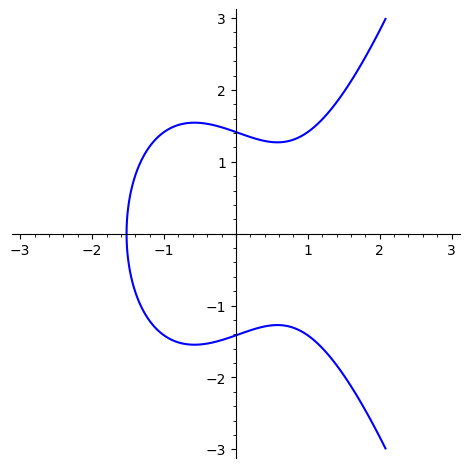
\includegraphics[scale=0.63]{assets/weiers_1.png}
        &
        
        \bigskip 
        
        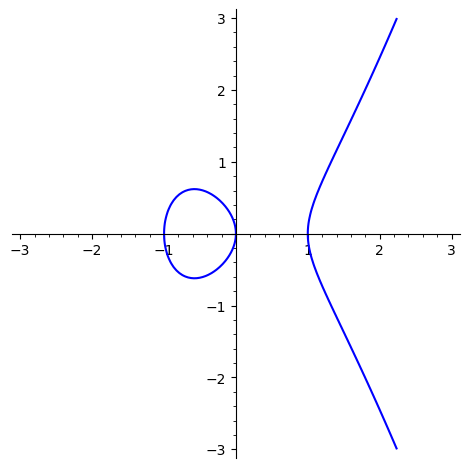
\includegraphics[scale=0.63]{assets/weiers_2.png}
    \end{tabular}
\end{center}
These curves have a lot of important geometry. 
\begin{itemize}
    \item Observe that they are symmetric about the $x$-axis, i.e., they have vertical symmetry. Stated formally, if $(x, y)$ is a point satisfying $y^2 + x^3 + ax + b$, then its reflection $(x, -y)$ across the $x$-axis is also a point satisfying the same equation. If $P = (x, y)$ is a point on a curve defined by a Weierstrass equation, we define\footnote{We only invert the $y$-coordinate of $P$ to get $-P$, not both coordinates.} $-P$ to be this reflection $(x, -y)$.  
    \item If we pick any two points on the curve, the unique line that passes through those two points will (almost) have a unique ``other'' point of intersection with the curve.
\end{itemize}

\begin{mdframed}
    (Example.) Suppose we have the Weierstrass equation $y^2 = x^3 + 17$. This is nonsingular because \[\Delta = -16(4 \cdot 0^3 + 27 \cdot 17^2) = -16 \cdot 27 \cdot 17^2 \neq 0.\]
    Consider the points $P = (-2, 3)$ and $Q = (-1, 4)$. Both of these lie on the curve (see exercise \textbf{A}). THere is a unique ``secant'' line that passes through these two points; we can calculate its slope using the usual slope formula, 
    \[m = \frac{4 - 3}{(-1) - (-2)} = 1,\]
    and then we can find the equation of the secant line itself using point-slope form: 
    \[y - 4 = 1 \cdot (x - (-1)) \implies y = x + 5.\]
    How do we intersect this secant line with the curbe? Remember that this will consist of all $(x, y)$ points that satisfy both $y = x + 5$ and $y^2 = x^3 + 17$, so substituting the first equation into the second gives us 
    \begin{equation*}
        \begin{aligned}
            y^2 &= x^3 + 17 \\ 
                &\implies (x+5)^2 = x^3 + 17 \\ 
                &\implies x^2 + 10x + 25 = x^3 + 17 \\ 
                &\implies x^3 - x^2 - 10x - 8 = 0.
        \end{aligned}
    \end{equation*}
    We now need to solve this cubic equation. This generally isn't easy, but remember that we know $x = -2$ and $x = -1$ must be solutions to this equation, since $P = (-2, 3)$ and $Q = (-1, 4)$ are on the curve and on the line, and the $x$-coordinates of these points are precisely $-2$ and $-1$, respectively. Therefore, we know that 
    \[(x + 2)(x + 1) = x^2 + 3x + 2\]
    must divide $x^3 - x^2 - 10x - 8$. We can use polynomial long division to find the quotient (see exercise \textbf{B}). 

    \bigskip 

    We find that $x^3 - x^2 - 10x - 8 = (x + 2)(x + 1)(x - 4)$, so indeed the third solution to the cubic equation is $x = 4$ and thus plugging in $x = 4$ into the equation of line yields the point $R = (4, 9)$ (see exercise \textbf{C}). 
\end{mdframed}

\begin{mdframed}
    (Exercise \textbf{A}.) Check that $P = (-2, 3)$ and $Q = (-1, 4)$ are both on the curve defined by $y^2 = x^3 + 17$. 

    \begin{mdframed}
        For $P = (-2, 3)$, we have $3^2 = (-2)^3 + 17 \implies 9 = -8 + 17 = 9$; because both sides are equal, this point is on the curve. 

        \bigskip 

        For $Q = (-1, 4)$, we have $4^2 = (-1)^3 + 17 \implies 16 = -1 + 17 = 16$, so again this point is on the curve.
    \end{mdframed}
\end{mdframed}

\begin{mdframed}
    (Exercise \textbf{B}.) Use polynomial long division to divide $x^3 - x^2 - 10x - 8$ by $x^2 + 3x + 2$ and check that the quotient is $x - 4$ and the remainder is 0.

    \begin{mdframed}
        After performing long division, we find that the result is $x - 4$: 

        \smallskip 

        \polylongdiv[style=A]{x^3 - x^2 - 10x - 8}{x^2 + 3x + 2}
    \end{mdframed}
\end{mdframed}

\begin{mdframed}
    (Exercise \textbf{C}.) Check that $R = (4, 9)$ is on the curve defined by $y^2 = x^3 + 17$. 

    \begin{mdframed}
        \[y^2 = 9^2 = 81,\]
        \[x^3 + 17 = 4^3 + 17 = 64 + 17 = 81,\]
        and since both sides are equal, $R$ is on the curve.
    \end{mdframed}
\end{mdframed}

This is essentially what the example we've just gone over does: 
\begin{center}
    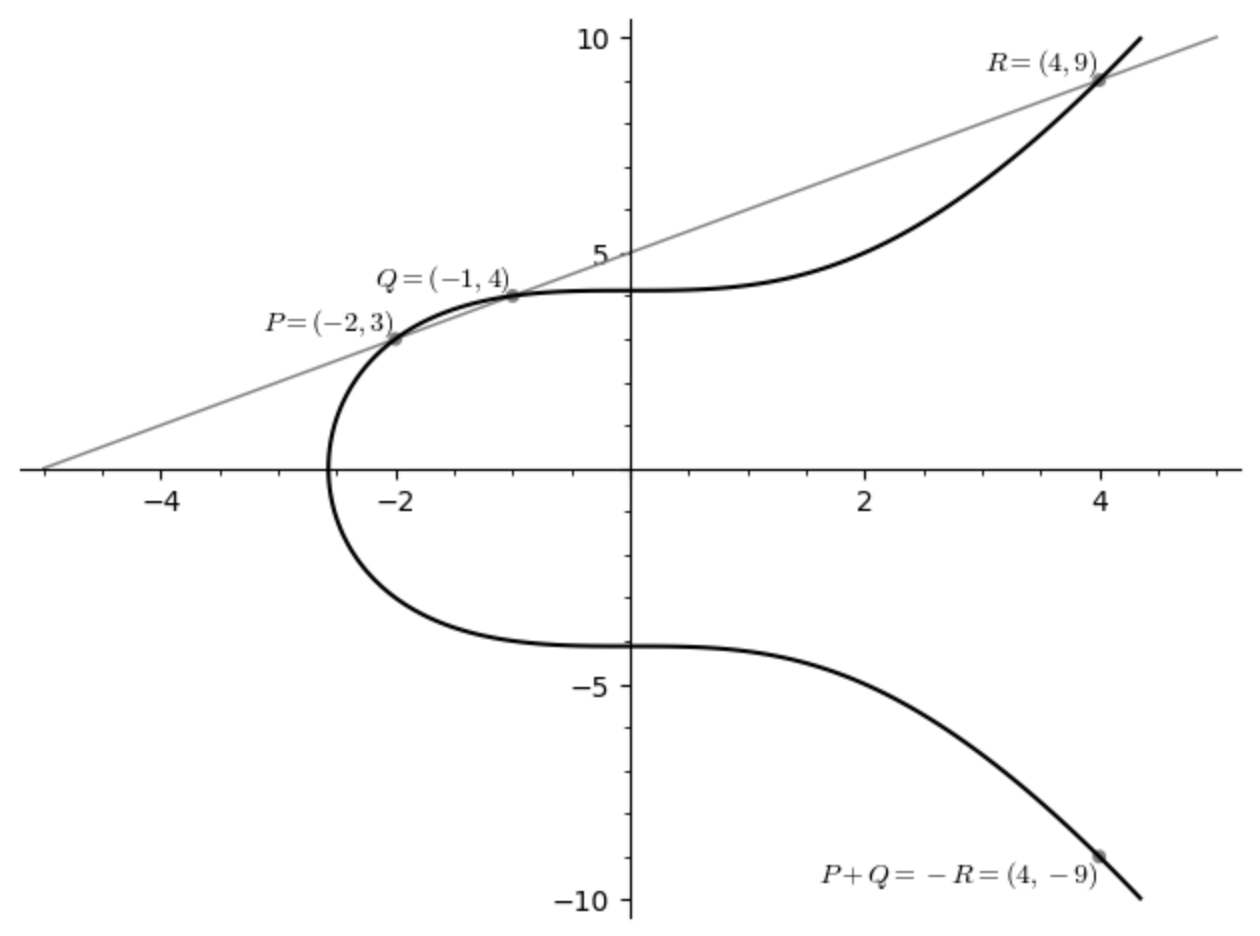
\includegraphics[scale=0.3]{assets/weiers_3.png}

    \emph{Taken from Professor Agrawal's Notes.}
\end{center}

Notice here that we defined $P + Q = -R = (4, -9)$. In reality, however, this process may be more complicated than simply adding the $x$ and $y$ coordinates of the two points. 

\begin{mdframed}
    (Exercise.) 
    \begin{enumerate}[(a)]
        \item Let $S = (2, 5)$. Check that $S$ is on the same curve $y^2 = x^3 + 17$. 
        \begin{mdframed}
            \[y^2 = 25\]
            and 
            \[x^3 + 17 = 25,\]
            so $S$ is also on this curve. 
        \end{mdframed}
        \item What is the third point of the intersection on between the curve $y^2 = x^3 + 17$ and the second line connecting $Q = (-1, 4)$ and $S$?
        \begin{mdframed}
            Given the two points $Q$ and $S$, we can find their slopes: 
            \[m = \frac{4 - 5}{(-1) - 2} = \frac{-1}{-3} = \frac{1}{3}.\]
            Once we have the slope, we can find the equation of the line that passes through both points: 
            \[y - 4 = \frac{1}{3}(x - (-1)) \implies y - 4 = \frac{1}{3}(x + 1) \implies y = \frac{1}{3}x + \frac{1}{3} + 4 \implies y = \frac{1}{3}x + \frac{13}{3}.\]
            Remember that the intersection of the curve and the secant line will consist of all points $(x, y)$ such that both $y = \frac{1}{3}x + \frac{13}{3}$ and $y^2 = x^3 + 17$ are satisfied, so 
            \[y^2 = x^3 + 17 \implies \left(\frac{1}{3}x + \frac{13}{3}\right)^2 = x^3 + 17 \implies x^3 - \frac{1}{9}x^2 - \frac{26}{9}x + 17 - \frac{169}{9} = 0.\]
            Since this is a cubic function, there are three solutions. We know that $x = -1$ and $x = 2$ are solutions to this equation, so we can use long division to find the last solution. In particular, by dividing $x^3 - \frac{1}{9}x^2 - \frac{26}{9}x + 17 - \frac{169}{9}$ by $(x - 2)(x + 1) = x^2 - x - 2$,  
            
            \smallskip 

            \polylongdiv[style=A]{x^3 - \frac{1}{9}x^2 - \frac{26}{9}x + 17 - \frac{169}{9}}{x^2-x-2}

            \smallskip 

            we find that $x = -\frac{8}{9}$ is the last root. So, plugging this root into the equation of the line gives us \[\frac{1}{3}\left(-\frac{8}{9}\right) + \frac{13}{3} = \frac{109}{27},\] thus $R = \left(-\frac{8}{9}, \frac{109}{27}\right)$.
        \end{mdframed}
        \item What is $Q + S$? 
        \begin{mdframed}
            We have \[Q + S = -R = \left(-\frac{8}{9}, -\frac{109}{27}\right).\]
        \end{mdframed}
        \item With $P = (-2, 3)$ and $R = (4, 9)$ on $y^2 = x^3 + 17$ as above, what is $P + R$? 
        \begin{mdframed}
            The slope of $P$ and $R$ is 
            \[m = \frac{9 - 3}{4 - (-2)} = \frac{6}{6} = 1,\]
            so the equation of the line that passes through both points is \[y - 9 = 1(x - 4) \implies y = x - 4 + 9 \implies y = x + 5.\]
            Plugging this secant line equation into the Weierstrass equation gives us 
            \[y^2 = x^3 + 17 \implies (x + 5)^2 = x^3 + 17 \implies x^3 - x^2 - 10x - 8 = 0.\]
            Knowing that the two solutions to the intersection of the curve and the secant line are $x = -2$ and $x = 4$, we know that $(x + 2)(x - 4) = x^2 - 2x - 8$ must divide $x^3 - x^2 - 10x - 8$, so 
            
            \polylongdiv[style=A]{x^3 - x^2 - 10x - 8}{x^2 - 2x - 8}

            and so the last root must be $x = -1$. Plugging this $x = -1$ back into the secant line yields $y = 4$, so in particular $T = (-1, 4)$. Therefore, 
            \[P + R = -T = (-1, 4).\]
        \end{mdframed}
    \end{enumerate}
\end{mdframed}
Remember how we mentioned the (almost) unique ``other'' point? There are several caveats to consider. 
\begin{itemize}
    \item Suppose we choose $P = (-2, 3)$, the same point from the example. What does it mean to pick $P + P$ or $2P$? There's not\footnote{This is a problem particularly because the first step of this process involves finding such a secant line.} a unique secant line that passes through $P$ and $P$. However, recall in calculus that, if we think about the secant line through two points on a curve, and take the limit as one of the two points approaches the other, what we end up with is the tangent line. So, we can use this. In other words, we can define $P + P$ by going through the same process as usual, but using the tangent line of the curve at $P$. 
    
    \bigskip 

    Consider again $y^2 = x^3 + 17$. Using implicit differentiation, we have 
    \[2y\frac{dy}{dx} = 3x^2.\]
    Then, with $P = (x, y) = (-2, 3)$, plugging this in gives us 
    \[2 \cdot 3 \cdot \frac{dy}{dx}\bigg\rvert_{P} = 3(-2)^2 \implies \frac{dy}{dx}\bigg\rvert_{P} = 2.\]
    Finding the equation of the tangent line again using point-slope form like we did gives us 
    \[y - 3 = 2(x - (-2)) \implies y = 2x + 7.\]
    From there, the usual process follows. It should be noted that the $x$ in the point will be a double root of the cubic since the line is tangent to the curve \emph{at} $P$. 

    \begin{mdframed}
        (Exercise.) On the curve $y^2 = x^3 + 17$, define $2S$ where $S = (2, 5)$. Calculate $2S$. 

        \begin{mdframed}
            We have $2y\frac{dy}{dx} = 3x^2$, so with $S = (x, y) = (2, 5)$, we have 
            \[2(5)\frac{dy}{dx}\bigg\rvert_{S} = 3(2)^2 \implies \frac{dy}{dx}\bigg\rvert_{S} = \frac{3(2)^2}{2(5)} = \frac{12}{10} = \frac{6}{5}.\] From there, we can find the equation of the secant line,
            \[y - 5 = \frac{6}{5}(x - 2) \implies y = \frac{6}{5}(x - 2) + 5 \implies y = \frac{6}{5}x + \frac{13}{5}.\]
            Plugging this back into the Weierstrass equation yields 
            \[\left(\frac{6}{5}x + \frac{13}{5}\right)^2 = x^3 + 17 \implies \frac{36}{25}x^2 + \frac{156}{25}x + \frac{169}{25} = x^3 + 17 \implies x^3 - \frac{36}{25}x^2 - \frac{156}{25}x + \frac{256}{25} = 0.\] 
            We know that $x = 2$ is the only root, so we know that this must be a double root. Thus, we know that $(x - 2)(x - 2) = x^2 - 4x + 4$ must divide $x^3 - \frac{36}{25}x^2 - \frac{156}{25}x + \frac{256}{25}$. Therefore, 

            \polylongdiv[style=A]{x^3 - \frac{36}{25}x^2 - \frac{156}{25}x + \frac{256}{25}}{x^2 - 4x + 4}

            and thus $x = -\frac{64}{25}$ is the other root. Plugging this back into the secant line gives us $y = -\frac{59}{125}$, thus $T = \left(-\frac{64}{25}, -\frac{59}{125}\right)$ and $2S = -T = \left(-\frac{64}{25}, \frac{59}{125}\right)$.
        \end{mdframed}
    \end{mdframed}

    \item There is one situation when the line passing through two points(either the secant line through two distinct points or the tangent line at a single point) does not have a third point of intersection with the curve. This happens when the line ends up being vertical. We can deal with this \emph{by fiat}; that is, we declare that there is a point $O$ called the \emph{point at infinity}, which is a point on the curve defined by $y^2 = x^3 + 17$ and is also a point on every vertical line in the plane. It is its own negative. So, when we try to ``add'' two points and encounter the situation where a secant or tangent line is vertical, we declare the sum to be $O$.
    
    \begin{definition}{Elliptic Curve}{}
        Fix a nonsingular Weierstrass equation $y^2 = x^3 + ax + b$. The \textbf{elliptic curve} $E$ defined by this equation is the set of points $(x, y)$ satisfying this equation, together with a \emph{point of infinity} denoted $O$ and assumed by fiat to 
        \begin{itemize}
            \item lie on the curve, 
            \item lie on every vertical line in the plane, and 
            \item be its own reflection across the $x$-axis. 
        \end{itemize}
    \end{definition}

    \begin{theorem}{}{3-10:2}
        Given any $P \in E$, where $E$ is an elliptic curve, we define $-P$ to be the reflection of $P$ across the $x$-axis. Given any two points $P, Q \in E$, there is a unique secant or tangent line passing through $P$ and $Q$, and this line has a unique third point of intersection with the curve; we define $P + Q$ to be the negative of this third point of intersection. Then, 
        \begin{itemize}
            \item Associativity: for any $P, Q, R \in E$, $(P + Q) + R = P + (Q + R)$.
            \item Commutativity: for any $P, Q \in E$, $P + Q = Q + P.$
            \item Identity: for any $P \in E$, $P + O = P.$
            \item Inverses: for any $P \in E$, $P + (-P) = O.$
        \end{itemize}
    \end{theorem}
    \textbf{Remark:} The above is saying that $E$ is an ``abelian'' group\footnote{If you've taken group theory, this should be familiar. Don't worry if you aren't familiar with this.}.
\end{itemize} 

\begin{theorem}{Elliptic Curve Addition Formula}{3-10:1}
    Suppose $P = (x_1, y_1)$ and $Q = (x_2, y_2)$ are both points on the curve $y^2 = x^3 + ax + b$. Then, define 
    \[\lambda = \begin{cases}
        \frac{y_2 - y_1}{x_2 - x_1} & \text{if } P \neq Q \\ 
        \frac{3x_1^2 + a}{2y_1} & \text{if } P = Q 
    \end{cases}.\]
    If $\lambda$ is defined (i.e., the denominator above is nonzero), then set 
    \[\nu = y_1 - \lambda x_1\]
    \[x_3 = \lambda^2 - x_1 - x_2\]
    \[y_3 = \lambda x_3 + \nu.\]
    Then, $P + Q = (x_3, -y_3)$. 
\end{theorem}

\begin{mdframed}
    (Exercise.) Consider the Weierstrass equation $y^2 = x^3 - 2x$. 

    \begin{enumerate}[(a)]
        \item Verify that this equation is nonsingular. Let $E$ be the corresponding elliptic curve. 
        \begin{mdframed}
            Computing the discriminant with $a = -2$ and $b = 0$ gives us
            \[\Delta = -16(4(-2)^3 + 27(0)^2) = -16 \cdot 4(-2)^3 \neq 0,\]
            so this equation is nonsingular. 
        \end{mdframed}
        \item Verify that $P = (0, 0)$ is on the curve. What is $2P$? 
        \begin{mdframed}
            The left-hand side has $0^2 = 0$ and the right-hand side has $0^3 - 2(0) = 0$, so it follows that $P$ is on the curve. 

            \bigskip 

            Note that, using implicit differentiation on the Weierstrass equation given, we find that $\frac{dy}{dx} 2y = 3x^2 - 2 \implies \frac{dy}{dx} = \frac{3x^2 - 2}{2y}$. Then, \[\frac{dy}{dx}\bigg\rvert_{P} = \frac{3(0)^2 - 2}{2(0)}.\] However, this is \emph{undefined}. Therefore, it follows that $2P = O$. 
        \end{mdframed}
        \item Verify that $Q = (-1, 1)$ is on the curve. What is $2Q$?
        \begin{mdframed}
            By the same process we used in the previous step, we can verify that $Q \in E$. Using the same implicit differentation we did in the previous step, we find that 
            \[\frac{dy}{dx}\bigg\rvert_{Q} = \frac{3(-1)^2 - 2}{2(1)} = \frac{3 - 2}{2} = \frac{1}{2}.\] While we can continue to find the secant line and whatnot, let's use (\ref{th:3-10:1}) to make this process a bit faster. We know that $Q = Q$, so
            \[\lambda = \frac{3(-1)^2 + (-2)}{2(1)} = \frac{3 - 2}{2} = \frac{1}{2}.\] Then, \[\nu = y_1 - \lambda x_1 = 1 - \frac{1}{2}(-1) = 1 + \frac{1}{2} = \frac{3}{2}.\]
            \[x_3 = \lambda^2 - x_1 - x_2 = \left(\frac{1}{2}\right)^2 - (-1) - (-1) = \frac{1}{4} + 2 = \frac{1}{4} + \frac{8}{4} = \frac{9}{4}.\]
            \[y_3 = \lambda x_3 + \nu = \frac{1}{2}\frac{9}{4} + \frac{3}{2} = \frac{9}{8} + \frac{12}{8} = \frac{21}{8}.\]
            Call this point $T$ so that $T = \left(\frac{9}{4}, \frac{21}{8}\right)$. Then, $2Q = -T = \left(\frac{9}{4}, -\frac{21}{8}\right)$.
        \end{mdframed}
        \item What is $P + Q$? 
        \begin{mdframed}
            With $P = (x_1, y_1) = (0, 0)$ and $Q = (x_2, y_2) = (-1, 1)$, we have 
            \[\lambda = \frac{1 - 0}{-1 - 0} = \frac{1}{-1} = -1.\]
            Then, 
            \[\nu = 0 - (-1)(0) = 0,\]
            \[x_3 = (-1)^2 - 0 - (-1) = 1 + 1 = 2,\]
            \[y_3 = -1(2) + 0 = -2.\]
            So, we know that $T = (2, -2) \in E$. Thus, $P + Q = -T = (2, 2)$.   
        \end{mdframed}
        \item What is $3Q$? 
        \begin{mdframed}
            We know that $3Q = Q + 2Q$. We can use the above theorem (elliptic curve addition) and our calculations from the previous part to compute this.
        \end{mdframed}
        \item What is $4Q$? 
        \begin{mdframed}
            We know that $4Q = 2Q + 2Q$. We can use the above theorem (elliptic curve addition) and our calculations from the previous part to compute this.
        \end{mdframed}
        \item What is $5Q$? 
        \begin{mdframed}
            We know that $5Q = 4Q + Q$.  We can use the above theorem (elliptic curve addition) and our calculations from the previous part to compute this.
        \end{mdframed}
    \end{enumerate}
\end{mdframed}

\begin{definition}{Order}{}
    Suppose $P$ is a point on an elliptic curve $E$. The order of $P$, denoted $\ord_{E}(P)$, is the smallest positive integer $n$ such that $nP = O$, if such an integer exists. Otherwise, the order of $P$ is $\infty$. 
\end{definition}

\begin{mdframed}
    (Exercise.) Let $E$ be the elliptic curve defined by the Weierstrass equation $y^2 = x^3 - 4x$. Find the order of the following points. 
    \begin{enumerate}[(a)]
        \item $P = (-2, 0)$
        \begin{mdframed}
            Starting with $P$, we note that 
            \[\frac{dy}{dx} 2y = 3x^2 - 4 \implies \frac{dy}{dx} = \frac{3x^2 - 4}{2y}.\] Because $y = 0$, it follows that, at the point $P$, there is a vertical tangent line and thus $1P = O$ and $n = 1$. 
        \end{mdframed}
        \item $Q = (0, 0)$
        \begin{mdframed}
            Note that $1Q = Q = (0, 0)$. Because this point has a vertical tangent line on the curve, it follows that $n = 1$.  
        \end{mdframed}
        \item $P + Q$
        \begin{mdframed}
            Let $P = (x_1, y_1) = (-2, 0)$ and $Q = (x_2, y_2) = (0, 0)$. Note that, using (\ref{th:3-10:1}), we find that $\lambda = \frac{0 - 0}{0 - (-2)} = \frac{0}{2} = 0$. Then, 
            \[\nu = 0 - 0(-2) = 0.\]
            \[x_3 = 0^2 - (-2) - 0 = 2.\]
            \[y_3 = 0(2) + 0 = 0.\]
            So, we find that $P + Q = (2, -0) = (2, 0)$. 
            
            \bigskip 

            We now want to compute $2(P + Q) = (P + Q) + (P + Q)$. Note that these points are obviously equal, so 
            \[\lambda = \frac{3(2)^2 - 4}{2(0)}.\]
            However, $\lambda$ is undefined, so it follows that $2(P + Q) = O$ and thus $n = 2$. 
        \end{mdframed}
    \end{enumerate}
\end{mdframed}


\subsection{Interlude: Elliptic Curves Mod a Prime}
We now fix a prime $p$. For technical reasons that are not worth lingering on for our purposes here, we assume\footnote{In applications to cryptography, $p$ will be very large anyways.} that $p \geq 5$. 

\begin{definition}{Integral Weierstrass Equation}{}
    A Weierstrass equation $y^2 = x^3 + ax + b$ is \textbf{integral} if $a$ and $b$ are integers. We then say that the equation is singular mod $p$ if $\Delta \equiv 0 \Mod{p}$. Otherwise, it is nonsingular mod $p$. 
\end{definition}

\begin{mdframed}
    (Example.) Suppose we have the Weierstrass equation $y^2 = x^3 + 17$. It is integral since $a = 0$ and $b = 17$ are integers. Then, we calculated earlier that \[\Delta = -16 \cdot 27 \cdot 17^2.\] The only primes this is divisible by are 2, 3, and 17. Thus, the equation $y^2 = x^3 + 17$ is singular mod $p = 17$, but nonsingular otherwise (recall that we are ruling out $p = 2, 3$).
\end{mdframed}

\begin{mdframed}
    For each of the following integral Weierstrass equations, find all primes $p \geq 5$ such that the equation is singular mod $p$. 
    \begin{enumerate}
        \item $y^2 = x^3 - 2x$    
        \begin{mdframed}
            With $a = -2$ and $b = 0$, we have $\Delta = -16(4(-2)^3 + 27(0)^2) = -16 \cdot 4(-2)^3 = -16 \cdot 4(-8) = 512$. Computing the prime factorization of 512 gives us 
            \[512 = 2^9.\]
            So, it follows that this equation is singular mod $p = 2$. With the limitation that $p \geq 5$, no prime will cause the equation to be singular. 
        \end{mdframed}
        \item $y^2 = x^3 + x + 1$
        \begin{mdframed}
            With $a = 1$ and $b = 1$, we have $\Delta = -16(4(1)^3 + 27(1)^2) = -16(4 + 27) = -16(31)$. The prime factorization of $\Delta$ is 
            \[-16(31) = -2^4 31^1,\]
            so the equation is singular mod $p$ when $p = 2$ or $p = 31$. With the limitation that $p \geq 5$, only $p = 31$ applies.
        \end{mdframed}
        \item $y^2 = x^3 - 1$
        \begin{mdframed}
            With $a = 0$ and $b = -1$, we have $\Delta = -16(4(0)^3 + 27(-1)^2) = -16(27).$ The prime factorization would be \[-16(27) = -2^4 3^3,\]
            so the equation is singular mod $p$ when $p = 2$ or $p = 3$. With the limitation that $p \geq 5$, no prime will cause the equation to be singular. 
        \end{mdframed}
    \end{enumerate}
\end{mdframed}
So, when we have an integral Weierstrass equation $y^2 = x^3 + ax + b$, we can consider its ``solutions mod $p$.'' By this, we mean integers $(x, y)$ such that $y^2 \equiv x^3 + ax + b \Mod{p}$. 

\begin{mdframed}
    (Example.) Suppose $p = 7$ and consider the Weierstrass equation $y^2 = x^3 + 17$. Then, $(1, 2)$ is a solution to the equation mod $p$ because 
    \[y^2 = 2^2 = 4 \equiv 18 = 1^3 + 17 = x^3 + 17 \Mod{7}.\]
\end{mdframed}
Let's define that, if $x, y, x', y'$ are all integers, then 
\[(x, y) \equiv (x', y') \Mod{p}\]
means that $x \equiv x' \Mod{p}$ and $y \equiv y' \Mod{p}$. Notice that, if $(x, y)$ is a solution mod $p$ of $y^2 = x^3 + ax + b$, then so is any pair of integers that is congruent mod $p$. 
\begin{mdframed}
    (Example.) In the above example, $(1, 9), (8, 2), (-6, 9)$ are all congruent mod 7 to $(1, 2)$, and they are all also solutions mod 7 to $y^2 = x^3 + 17$. 
\end{mdframed}    
We'll typically consider only solutions $(x, y)$ where $0 \leq x, y < p$ in order to avoid having to list off all the congruent solutions.

\begin{theorem}{}{}
    Suppose $y^2 = x^3 + ax + b$ is an integral Weierstrass equation which is nonsingular mod $p$. The corresponding elliptic curve mod $p$ is the set $E$ of solutions mod $p$ to the equation, together with an extra point at infinity called $O$. 

    \bigskip 

    Suppose $P \in E$. We define $-P$ as follows: 
    \begin{itemize}
        \item If $P = O$, then $-P = O$ as well.
        \item If $P = (x, y)$, then $-P = (x, -y \Mod{p})$. 
    \end{itemize}
    Then, $-P$ is in fact an element of $E$. 

    \bigskip 

    Moreover, suppose $P, Q \in E$. We define $P + Q$ as follows: 
    \begin{itemize}
        \item If $P = O$, then $P + Q = Q$. 
        \item If $Q = O$, then $P + Q = P$. 
        \item If $P = (x_1, y_1)$ and $Q = (x_2, y_2)$ are both solutions mod $p$ of $y^2 = x^3 + ax + b$, then 
        \begin{itemize}
            \item If $P \neq Q$ and $x_2 - x_1$ is not invertible mod $p$, set \[P + Q = O.\]
            \item If $P = Q$ and $y_1$ is not invertible mod $p$, set $P + Q = 2P = O$. 
            \item Otherwise, define\footnote{You compute the inverse mod $p$ first, and then multiply that and mod that by $p$.}
            \[\lambda = \begin{cases}
                (y_2 - y_1)(x_2 - x_1)^{-1} \Mod{p} & \text{if } P \neq Q \\ 
                (3x_1^2 + a)(2y_1)^{-1} \Mod{p} & \text{if } P = Q 
            \end{cases}.\]
            Then, set 
            \[\nu = y_1 - \lambda x_1 \Mod{p}\]
            \[x_3 = \lambda^2 - x_1 - x_2 \Mod{p}\]
            \[y_3 = \lambda x_3 + \nu \Mod{p}\]
            Then, $R = (x_3, y_3)$ is a solution mod $p$ and we define $P + Q = -R = (x_3, -y_3 \Mod{p})$. 
        \end{itemize}
    \end{itemize}
    Then, 
    \begin{itemize}
        \item Associativity: for any $P, Q, R \in E$, $(P + Q) + R = P + (Q + R)$.
        \item Commutativity: for any $P, Q \in E$, $P + Q = Q + P.$
        \item Identity: for any $P \in E$, $P + O = P.$
        \item Inverses: for any $P \in E$, $P + (-P) = O.$
    \end{itemize}
\end{theorem}

\begin{mdframed}
    (Example.) Consider $p = 7$ and $y^2 = x^3 + 17 \equiv x^3 + 3 \Mod{7}$. We already saw that $P = (1, 2)$ is a solution to this equation. We also know that $Q = (3, 4)$ is also a solution to this equation. With this in mind, how do we compute $P + Q$ in ``two'' different ways?
    \begin{itemize}
        \item Using the above formula carefully, notice that $P \neq Q$ and $x_2 - x_1 = 3 - 1 = 2$ is invertible mod 7 because $\gcd(2, 7) = 1$. Its inverse\footnote{Generally, you would want to use the extended Euclidian algorithm.} is 4. Thus, 
        \[\lambda = (y_2 - y_1)(x_2 - x_1)^{-1} \Mod{p} = (4 - 2)(3 - 1)^{-1} \Mod{7} = 2 \cdot 4 \Mod{7} = 1.\]
        From there, 
        \[\nu = y_1 - \lambda x_1 \Mod{p} = 1\]
        \[x_3 = \lambda^2 - x_1 - x_2 \Mod{p} = 4\]
        \[y_3 = \lambda x_3 + \nu \Mod{p} = 5.\]
        Therefore, $R = (4, 5)$ and $P + Q = -R = (4, -5 \Mod{7}) = (4, 2)$. 

        \item The other way is to remember the geometry that underlies these formulas and use the geometry to guide your calculations. Just remember that you're trying to do everything mod 7. So, begin by computing the slope of the two points using rise-over-run, but since we need to do this calculation mod 7, isntead of dividing, we multiply by a modular inverse. In other words, we compute 
        \[m = (4 - 2)(3 - 1)^{-1} = 2 \cdot 2^{-1} \equiv 2 \cdot 4 = 8 \equiv 1 \Mod{7}.\]
        This is the same value we found with $\lambda$ above. Now, the next step is to use the point-slope form to find the equation of the secant line; we know that it has slope 1, and it passes through the point $(1, 2)$, so its equation should be \[y - 2 = 1(x - 1) \implies y = x + 1.\]
        The $y$-intercept here matches what we computed for $\nu$ above. We now want to intersect this secant line with the curve. So, we substitute $y = x + 1$ into $y^2 = x^3 + 3$ and get \[x^3 - x^2 - 2x + 2 = 0.\]
        We now need to find the roots of this cubic mod 7. We know that 1 and 3 are roots, so $(x - 1)(x - 3) = x^2 - 4x + 3$ must divide this cubic. Performing polynomial long division ``mod 7'' gives us $x - 4$ as the result, so the third point of intersection of the secant line must have $x = 4$, so $y = 5$. This gives us $R = (4, 5)$. Therefore, 
        \[P + Q = (1, 2) + (3, 4) = (4, -5 \Mod{7}) = (4, 2).\]
    \end{itemize}
\end{mdframed}

\begin{definition}{Order}{}
    Suppose $P$ is a point on an elliptic curve $E$ mod $p$. The \textbf{order} of $P$, denoted $\ord_{E}(P)$, is the smallest positive integer $n$ such that $nP = O$. 
\end{definition}
Unlike in the real case, we don't need to worru about the infinite order anymore. 

\bigskip 

We also have the analogs of the First and Second Lemmas about Orders. 
\begin{lemma}{First Lemma About Orders for Elliptic Curves}{}
    Let $E$ be an elliptic curve mod $p$ and suppose $P \in E$. If $mP = O$, then $\ord_{E}(P)$ divides $m$. 
\end{lemma}

\begin{lemma}{Second Lemma About Orders for Elliptic Curves}{}
    Let $E$ be an elliptic curve mod $p$ and suppose $P \in E$. Let $k = \ord_{E}(P)$. Then, \[iP \equiv jP \Mod{p}\] if and only if $i \equiv j \Mod{k}$. In particular, the points $O, P, 2P, 3P, \hdots, (k - 1)P$ are all incongruent mod $p$.
\end{lemma}
Having developed this theory, we can now state the basic problem that underlies elliptic curve cryptography. 
\begin{mdframed}
    (Elliptic Curve Discrete Logarithm Problem.) Suppose that you're given a prime $p$, an elliptic curve $E \Mod{p}$, and a point $P \in E$. Further suppose that $Q \in E$ is known to be a multiple of $P$. Find the discrete logarithm base $P$ of $Q$, i.e., the unique integer $k$ such that $0 \leq k < \ord_{E}(P)$ such that $Q = mP$. 
\end{mdframed}
The naive method for doing this is to just try all values of $k$ starting from $k = 0$ to $k = \ord_{E}(P) - 1$, but if $\ord_{E}(P)$ is very large, then this will be very slow. There are no methods that can help us find $k$ substantially faster in general, so we can choose $p, E, P$ in a way that makes the Elliptic Curve Discrete Logarithm Problem intractable for an adversary. 


\subsection{Elliptic Curve Diffie-Hellman}
Suppose Alice and Bob publicly agree to fix a prime $p$, an elliptic curve $E$ mod $p$ (specified by integers $a, b$ such that the Weierstrass equation $y^2 = x^3 + ax + b$ is nonsingular mod $p$), and a point $P \in E$. To ensure security, we need for $\ord_{P}(E)$ to be large. The data $(p, E, P)$ is all shared publicly.

\bigskip 

Alice can choose a secret integer $0 \leq k_a < \ord_{E}(P)$ and send Bob $Q_a = k_a P$. She can compute this value quickly using binary multiplication. Similarly, Bob can choose a secret integer $0 \leq k_b < \ord_{E}(P)$ and send Alice $Q_b = k_b P$. Alice computes $R = k_a Q_b$ and Bob computes $R = k_b Q_a \Mod{p}$. The two values of $R$ that Alice and Bob compute are the same since \[k_a Q_b = k_a (k_b P) = k_a k_b P = k_b (k_a P) = k_b Q_a.\]
Thus, Alice and Bob now share a secret point $R$ on the elliptic curve. 

\begin{mdframed}
    (Exercise.) Suppose Alice and Bob publicly agree to use the elliptic curve $y^2 = x^3 + 17 \Mod{p = 7}$ and the point $P = (1, 2)$. 
    \begin{enumerate}[(a)]
        \item Suppose Alice picks the number $k_a = 4$. What is the message $Q_a$ that she sends Bob? 
        \begin{mdframed}
            We know that \[Q_a = k_a P = 4P.\] Given this, we need to compute $4P$. Let's begin with $2P = P + P$. We know that $P = P$ and $y_1 = 2$ is invertible mod 7, so we define 
            \[\lambda = (3(1)^2 + 0)(2(2))^{-1} \Mod{7} = (3)((4)^{-1} \Mod{7}).\]
            Computing the inverse of 4 mod 7 gives us 2, so 
            \[\lambda = 3(2) \Mod{7} = 6 \Mod{7}.\]
            Then, we have 
            \[\nu = 2 - 6(1) = -4 \Mod{7} = 3\]
            \[x_3 = 6^2 - 1 - 1 = 34 \Mod{7} = 6\]
            \[y_3 = 6(6) + 3 = 39 \Mod{7} = 4.\]
            Therefore, we can define $R = (6, 4)$ and thus $P + P = -R = (6, -4 \Mod{7}) = (6, 3)$. Now that we have $2P$, we can compute $4P = 2P + 2P$. We know that $y_1 = 3$ is invertible mod 7, so 
            \[\lambda = (3(6)^2 + 0)(2(3))^{-1} \Mod{7} = (108)(6)^{-1} \Mod{7}.\]
            Computing the inverse of 6 mod 7 gives us 6, so 
            \[\lambda = 108(6) \Mod{7} = 4.\]
            Then, we have 
            \[\nu = 3 - 4(6) \Mod{7} = 0\]
            \[x_3 = 4^2 - 6 - 6 \Mod{7} = 4\]
            \[y_3 = 4(4) + 0 \Mod{7} = 2.\]
            Therefore, we can define $R = (4, 2)$ and thus $2P + 2P = -R = (4, -2 \Mod{7}) = (4, 5)$.
        \end{mdframed}
        \item Suppose Alice receives the point $Q_b = (5, 3)$ from Bob. What is her shared secret with Bob?
        \begin{mdframed}
            We know that 
            \[R = k_a Q_b = k_a (5, 3).\] 
        \end{mdframed}
    \end{enumerate}
\end{mdframed}

\begin{mdframed}
    (Exercise.) Suppose Alice and Bob publicly agree to use the elliptic curve $y^2 = x^3 + 17 \Mod{p} = 7$ and the point $P = (1, 2)$. This point has order 13, which is too small to be secure. Suppose Eve intercepts Alice and Bob's message: she sees that Alice sent Bob $Q_a = (3, 3)$ and that Bob sent Alice $Q_b = (6, 4)$. What is Alice and Bob's shared secret? 
    \begin{mdframed}
        
    \end{mdframed}
\end{mdframed}

\subsection{Interlude: Quadratic Residues}
A familiar feature of the real numbers is that some numbers do not have square roots (e.g., the negatives). The same thing happens when you mod an integer. For example, let $n = 5$. We know that the integer is congruent to 0, 1, 2, 3, or 4 mod 5. This means that any square must be congruent to $0^2 = 0$, $1^2 = 1$, $2^2 = 4$, $3^2 \equiv 4 \Mod{5}$, or $4^2 \equiv 1 \Mod{5}$. In other words, only 0, 1, or 4 have square roots mod 5, and 2 and 3 do not.

\begin{definition}{Quadratic Residue}{}
    Fix a positive integer $n$. We say that an integer $a$ is a \textbf{quadratic residue mod }$n$ if it has a square root mod $n$, i..e, if there exists an integer $x$ such that $x^2 \equiv a \Mod{n}$. 
\end{definition}

\begin{mdframed}
    (Exercise.) Find all quadratic residues mod the following integers. 
    \begin{enumerate}[(a)]
        \item $n = 3$
        \begin{mdframed}
            
        \end{mdframed}
        \item $n = 7$
        \begin{mdframed}
            
        \end{mdframed}
        \item $n = 11$
        \begin{mdframed}
            
        \end{mdframed}
    \end{enumerate}
\end{mdframed}

We'll see below that it will be useful to quickly determine whether an integer $a$ is a quadratic residue mod $a$ prime $p \geq 3$. It turns out that there is a good way to do this; let's introduce the following notation. 
\begin{definition}{Legendre Symbol}{}
    Let $p \geq 3$ be prime. For any integer $a$, define the Legendre symbol $(a/n)$ by 
    \[\left(\frac{a}{n}\right) = \begin{cases}
        0 & \text{if } a \equiv 0 \Mod{p} \\ 
        1 & \text{if } a \not\equiv 0 \Mod{p} \text{ and } a \text{ is a quadratic residue mod } p \\ 
        -1 & \text{if } a \not\equiv 0 \Mod{p} \text{ and } a \text{ is not a quadratic residue mod } p
    \end{cases}\]
\end{definition}
For example, we saw above that 4 is a quadratic residue mod 5, so 
\[\left(\frac{4}{5}\right) = 1\]
and we saw that 2 is not a quadratic residue mod 5, so 
\[\left(\frac{2}{5}\right) = -1.\]
We can now rephrase our goal: we would like a quick way of computing Legendre symbols. This is provided to us by combining binary exponentiation with the following: 
\begin{lemma}{Euler's Criterion}{}
    Let $p \geq 3$ be prime. For any integer $a$, 
    \[\left(\frac{a}{n}\right) \equiv a^{\frac{p - 1}{2}} \Mod{p}.\]
\end{lemma}

Euler's Criterion means that we have an efficient algorithm for determining whether something is a quadratic residue: we simply use binary exponentiation to compute $a^{(p - 1) / 2} \Mod{p}$ and we can read off the answer. 

\begin{mdframed}
    (Example.) Suppose we want to know if $a = 37$ is a quadratic residue mod $p = 97$. We have $(p - 1) / 2 = 96 / 2 = 48$, so we compute $a^{(p - 1) / 2} = 37^{48} \Mod{97}$ using binary exponentiation, and we find that it is $96 \equiv -1 \Mod{97}.$ Euler's Criterion says that 
    \[\left(\frac{37}{97}\right) \equiv 37^{(97 - 1) / 2} = 37^{48} \equiv -1 \Mod{97}.\]
    Therefore, 37 is not a quadratic residue mod 97. 
\end{mdframed}

\begin{mdframed}
    (Exercise.) Use Euler's Criterion to determine whether or not the following integers $a$ are quadratic residues mod $p = 19$. 
    \begin{enumerate}[(a)]
        \item $a = 3$
        \begin{mdframed}
            
        \end{mdframed}
        \item $a = 5$
        \begin{mdframed}
            
        \end{mdframed}
        \item $a = 11$
        \begin{mdframed}
            
        \end{mdframed}
    \end{enumerate}
\end{mdframed}


\subsection{Elliptic Curve Elgamal}
There is a variant of the Elgamal cryptosystem using elliptic curves that can be used to exchange messages, but there is a nontrivial encoding step. To make Elgamal work with elliptic curves, we first need a way to encode a plaintext message as a point on an elliptic curve $E$ mod $p$. 

\bigskip 

For this, there's a probablistic algorithm that encodes plaintext as $x$-coordinate of a plain (but note that not every integer will occur as the $x$-integer of a point on an elliptic curve mod $p$). Specifically, if $E$ is given by $y^2 = x^3 + ax + b$ and if $P = (x, y)$ is a point on the curve, then the $x$-coordinate must have the property that $x^3 + ax + b$ is a quadratic residue mod $p$. 

\subsubsection{The Process}
Suppose Bob wants to receive messages of length $N$. 
\begin{enumerate}
    \item Bob will fix a positive integer $s$. We'll see that, the larger Bob chooses the integer, the higher the probability that encoding will succeed. 
    \item Bob will then choose a prime $p > s26^N$ and an elliptic curve $E$ mod $p$ (defined by integers $a, b$ such that the integral Weierstrass equation $y^2 = x^3 + ax + b$ is nonsingular mod $p$), and a point $P \in E$. 
    \item He then computes $\ord_{E}(P)$. 
    \item Then, Bob chooses a secret integer $0 \leq k < \ord_{E}(P)$ to serve as his private key. He computes $Q = kP$, and this value is part of his public key. 
\end{enumerate}
In other words, Bob will share all of the data $(s, E, P, \ord_{E}(P), Q)$ publicly, and keep only the integer $k$ secret.

\bigskip 

Suppose now that Alice wants to send Bob a message.
\begin{enumerate}
    \item She converts her message into an integer $m$ using the same base 26 idea we used for RSA. 
    \item She will then iterate through values of $r = 0, 1, 2, \hdots, s - 1$ until she finds the first value of $x = sm + r$ such that\footnote{Remember that this is the \textbf{Legendre Symbol}!}
    \[\left(\frac{x^3 + ax + b}{p}\right) \neq -1.\]
    Note that the maximum possible value of $m$ is $26^N - 1$, so 
    \[x = sm + r < s(26^N - 1) + s = s26^N < p\]
    since Bob chose $p$ to be larger than $s26^N$. There is a roughly $1/2$ chance that an integer in $[0, p)$ is not a quadratic residue mod $p$, and here we are iterating through $s$ integers in the range $[0, p)$, so there is a $\left(\frac{1}{2}\right)^s$ chance that $x^3 + ax + b$ is not a quadratic residue for any of the $s$ possible values of $x = sm + r$. If none of the $s$ integers are quadratic residues, encoding fails. However, if Bob chose $s$ to be even moderately large, encoding failure is very unlikely. If encoding does fail, Alice can just modify her message slightly\footnote{Rephrasing slightly or adding a nonsense letter.} and try encoding again. 
    
    \item Once Alice finds a value of $x$ such that $x^3 + ax + b$ is a quadratic residue mod $p$, then there is an integer $y$ such that $y^2 \equiv x^3 + ax + b \Mod{p}$, so the point $M = (x, y)$ is on $E$. This will be the \underline{encoding} of her plaintext.
\end{enumerate}
This is not the ciphertext, but she can now encrypt the encoded message using a process very similar to the Elgamal cryptosystem we discussed earlier. 
\begin{enumerate}
    \item First, Alice chooses an ``ephemeral key'' $h$ such that $0 \leq h < \ord_{E}(P)$.
    \item She computes $S = hQ$, $R_1 = hP$, and $R_2 = M + S$. The pair, $(R_1, R_2)$, is the ciphertext she sends to Bob. 
\end{enumerate}
To decrypt the ciphertext $(R_1, R_2)$, Bob uses his private key $k$ to compute $S = kR_1$. Observe that 
\[kR_1 = k(hP) = khP = h(kP) = hQ,\]
so Bob has found the same value of $S$ that Alice had, even though he does not know the value of the ephemeral key $h$. He can then compute $-S$ by negating the $y$-coordinate, and he then calculates 
\[R_2 - S = R_2 + (-S) = (M + S) + (-S) = M + (S + (-S)) = M + O = M.\]
He has thus recovered Alice's encoded plaintext. 

\bigskip 

Finally, Bob just needs to decode $M$. If $M = (x, y)$, he can extract the first coordinate $x$. The quotient when he divides this by $s$ is the integer $m$ that represents the message in base 26, so he then finishes off by converting back to text using the same process we used for RSA above. 

\subsubsection{Encoding and Decoding}
\begin{mdframed}
    (Exercise.) Suppose Bob's public key has $s = 2$, $p = 97$, $a = 31$, and $b = 20$. The elliptic curve $E$ is then the one given by $y^2 = x^3 + 31x + 20 \Mod{p = 97}$. 
    \begin{enumerate}[(a)]
        \item What is the encoding of the plaintext message \code{B}? Follow the process above to find the corresponding point $M \in E$. 
        \begin{mdframed}
            First, we encode \code{B} into base 26; this gives us $m = 1$. Then, we need to iterate through all $r$ such that $0 \leq r \leq 2 - 1 = 1$. We find that 
            \begin{itemize}
                \item For $r = 0$, we have $x = 2(1) + 0 = 2$ and 
                \begin{equation*}
                    \begin{aligned}
                        \left(\frac{2^3 + 31(2) + 20}{97}\right) &= \left(\frac{90}{97}\right) \\ 
                            &= 90^{\frac{97 - 1}{2}} \Mod{97} \\ 
                            &= 90^{\frac{96}{2}} \Mod{97} \\ 
                            &= 90^{48} \Mod{97}.
                    \end{aligned}
                \end{equation*}
                With this in mind, we find that $90^{48} \equiv 96 \equiv -1 \Mod{97}$, so $r = 0$ is not an option. 

                \item For $r = 1$, we have $x = 2(1) + 1 = 3$ and 
                \begin{equation*}
                    \begin{aligned}
                        \left(\frac{3^3 + 31(3) + 20}{97}\right) &= \left(\frac{140}{97}\right) \\ 
                            &= 140^{\frac{97 - 1}{2}} \Mod{97} \\ 
                            &= 140^{48} \Mod{97} \\ 
                            &= 1 \Mod{97}.
                    \end{aligned}
                \end{equation*}
                Here, we find that $r = 1$ and thus $x = 3$ \emph{is} the option. 
            \end{itemize}
            Now that we have $x = 3$, we can compute \[y^2 \equiv 3^3 + 31(3) + 20 \Mod{97}.\] We find that $y \equiv 25$. Thus, \[M = (3, 25).\]
        \end{mdframed}
        \item Show that the encoding fails for the letter \code{K}. 
        \begin{mdframed}
            Encoding \code{K} gives us $m = 10$. Then, iterating through all $0 \leq r \leq 2 - 1 = 1$, we have 
            \begin{itemize}
                \item For $r = 0$, we have $x = 2(10) + 0 = 20$ and 
                \begin{equation*}
                    \begin{aligned}
                        \left(\frac{20^3 + 31(20) + 20}{97}\right) &= \left(\frac{8640}{97}\right) \\ 
                            &= 8640^{\frac{97 - 1}{2}} \Mod{97} \\ 
                            &= 8640^{48} \Mod{97} \\ 
                            &= 7^{48} \Mod{97} \\ 
                            &= 96 \Mod{97}.
                    \end{aligned}
                \end{equation*}
                This gives us $8640^{48} \equiv 96 \equiv -1 \Mod{97}$, so $r = 0$ is not an option. 

                \item For $r = 1$, we have $x = 2(10) + 1 = 21$ and 
                \begin{equation*}
                    \begin{aligned}
                        \left(\frac{21^3 + 31(21) + 21}{97}\right) &= \left(\frac{9933}{97}\right) \\ 
                            &= 9933^{\frac{97 - 1}{2}} \Mod{97} \\ 
                            &= 9933^{48} \Mod{97} \\ 
                            &= 39^{48} \Mod{97} \\ 
                            &= 96 \Mod{97}.
                    \end{aligned}
                \end{equation*}
                Once again, this gives us $9933^{48} \equiv 96 \equiv -1 \Mod{97}$, so $r = 1$ is not an option. 
            \end{itemize}
            Because we got $-1$ for all valid $r$, encoding is not possible.  
        \end{mdframed}
        \item Follow the process described above to find the plaintext message that results from decoding the point $(25, 30) \in E$.
        \begin{mdframed}
            TODO % ask about this
        \end{mdframed}
    \end{enumerate}
\end{mdframed}

\end{document}